%
% This document is available under the Creative Commons Attribution-ShareAlike
% License; additional terms may apply. See
%   * http://creativecommons.org/licenses/by-sa/3.0/
%   * http://creativecommons.org/licenses/by-sa/3.0/legalcode
%
% Copyright 2010 Jérôme Pouiller <jezz@sysmic.org>
%

% Pour faire une version imprimable, avec les notes sans overlay
% \PassOptionsToClass{notes=show,handout}{beamer}
% Pour en faire un article:
% \documentclass[10pt,ucs,usepdftitle=false,a4paper]{article}
% \usepackage{beamerarticle}

\documentclass[10pt,ucs,usepdftitle=false]{beamer}

% Pour mettre deux pages sur une
% (Préférer l'utilisation d'un post processing)
%\usepackage{pgfpages}
%\pgfpagesuselayout{2 on 1}[a4paper,border shrink=5mm]
%\pgfpagesuselayout{4 on 1}[a4paper,landscape, border shrink=5mm]
%\setbeameroption{show notes on second screen=right}

%
% This document is available under the Creative Commons Attribution-ShareAlike
% License; additional terms may apply. See
%   * http://creativecommons.org/licenses/by-sa/3.0/
%   * http://creativecommons.org/licenses/by-sa/3.0/legalcode
%
% Copyright 2010 Jérôme Pouiller <jezz@sysmic.org>
%

% Configurationde de Beamer

\usetheme{Warsaw}

% Quiris
%\usecolortheme[RGB={238,127,0}]{structure}
% Apollo
%\usecolortheme[RGB={0,56,126}]{structure}
% Sysmic
\usecolortheme[RGB={181,0,0}]{structure}

% Headers et footers
\useoutertheme[subsection=false]{smoothbars}
% Rectangle dans les itemize
\useinnertheme{rectangles}
% Pas de symboles pour la navigation
\setbeamertemplate{navigation symbols}{}

% Logo en filigranne
% \setbeamertemplate{background canvas}{
%   \tikz {
%     \node at (0,0) {};
%     \node[inner sep=0pt, opacity=0.2] at (0.5\paperwidth,-0.8\paperheight) {
\includegraphics[height=23.4mm,width=128mm]{pics/logo}};
%   }
% }

% Ajout des numéros de pages
\newcommand*\oldinsertshortitle{}%
\let\oldinsertshorttitle\insertshorttitle%
\renewcommand*\insertshorttitle{\oldinsertshorttitle\hfill\insertframenumber\,/\,\inserttotalframenumber}

\usepackage{ucs}              % La sortie est en UTF8
\usepackage[utf8x]{inputenc}  % L'entrée aussi
\usepackage[T1]{fontenc}      % Pour la césure des mots accentués
\usepackage{lmodern}          % Pour les lettres francaises
\usepackage[french]{babel}    % Pour la sortie francaise
\usepackage{times}
\usepackage{mathptmx}         % Font (don't forget to install latex-font-recommended)

% This document is available under the Creative Commons Attribution-ShareAlike
% License; additional terms may apply. See
%   * http://creativecommons.org/licenses/by-sa/3.0/
%   * http://creativecommons.org/licenses/by-sa/3.0/legalcode
%
% Copyright 2010 Jérôme Pouiller <jezz@sysmic.org>
%

\usepackage{tikz}
\usetikzlibrary{patterns}
\usetikzlibrary{shapes}
\usetikzlibrary{decorations}
\usetikzlibrary{positioning}
\usetikzlibrary{calc}

\tikzstyle{cgreen}  = [fill=green!20!white,  draw=green!50!black,  line width=1pt, rounded corners=1pt]
\tikzstyle{cred}    = [fill=red!20!white,    draw=red!50!black,    line width=1pt, rounded corners=1pt]
\tikzstyle{cblue}   = [fill=blue!20!white,   draw=blue!50!black,   line width=1pt, rounded corners=1pt]
\tikzstyle{cpurple} = [fill=purple!20!white, draw=purple!50!black, line width=1pt, rounded corners=1pt]
\tikzstyle{corange} = [fill=orange!20!white, draw=orange!50!black, line width=1pt, rounded corners=1pt]
\tikzstyle{ccyan}   = [fill=cyan!20!white,   draw=cyan!50!black,   line width=1pt, rounded corners=1pt]
\tikzstyle{cbrown}  = [fill=brown!20!white,  draw=brown!50!black,  line width=1pt, rounded corners=1pt]
\tikzstyle{cyellow} = [fill=yellow!20!white, draw=yellow!50!black, line width=1pt, rounded corners=1pt]

\def\timeline#1#2#3{
  \draw[xstep=1,ystep=1.5,gray,very thin] (0,0) grid (#1.5,#2);
  \draw[->, line width=1pt] (0,#2) -- (#1.5,#2) coordinate (x axis);
  \draw[line width=1pt] (0,#2) -- (0,0) coordinate (x axis);
  \foreach \x in {0,1,...,#1}
    \draw (\x,#2) node[anchor=north] {\tiny\x};
  \foreach \y/\ytext in {#3}
    \draw (0,\y) node[anchor=east] {\ytext};
}

\def\lo#1{ -- ++(#1,0) }
\def\hi#1{ |- ++(#1,1) -- ++(0,-1) }
\def\hop#1#2{\lo{#1}\hi{#2}}

% Period End
\def\pe#1#2#3{
   \begin{scope}
     \clip  (#1 - 0.2, #2 - 0.2) rectangle (#1, #2 + 0.2);
     \draw[#3] (#1, #2) circle (3pt);
   \end{scope}
}

% Period Begin
\def\pb#1#2#3{
   \begin{scope}
     \clip  (#1 + 0.2, #2 - 0.2) rectangle (#1, #2 + 0.2);
     \draw[#3] (#1, #2) circle (3pt);
   \end{scope}
}

% Period Begin and End
\def\p#1#2#3{
   \draw[#3] (#1, #2) circle (3pt);
}



\ifpdf
  \usepackage{embedfile} 
\else
  \newcommand{\embedfile}[1]{}
\fi

\usepackage[sections,displaymath]{preview}
\PreviewEnvironment{tikzpicture}
\PreviewEnvironment{center}
\PreviewEnvironment{frame}

\usepackage{hyperref} % Doit être chargé avant ntheorem
%\usepackage{realboxes} % Pour \Colorbox
\newcommand{\email}[1]{\href{mailto:#1}{\nolinkurl{<#1>}}}
\newcommand{\man}[1]{\emph{#1}}
\newcommand\file[1]{\lstinline[backgroundcolor=\color{{rgb}{1,1,0.8}},language=]{#1}}
\newcommand\cmd[1]{\lstinline[backgroundcolor=\color{{rgb}{1,1,0.8}},language=]{#1}}
\renewcommand\c[1]{\lstinline[backgroundcolor=\color{{rgb}{1,1,0.8}},language=c]{#1}}

\usepackage[newcommand]{ragged2e}

% \usepackage[]{version} 
% \usepackage{ntheorem} 
% \setlength{\theorempreskipamount}{0.8ex plus 0.9ex minus 0.1ex}
% \setlength{\theorempostskipamount}{0.8ex plus 0.9ex minus 0.1ex}
% \theoremprework{\vspace{3mm}\hrule}
% \theorempostwork{\hrule\vspace{3mm}}
% \theorembodyfont{\itshape}
% \theoremseparator{.}
% \newtheorem{quest}{Question}[section]

% \theorembodyfont{\normalfont}
% \theoremseparator{}
% \theoremstyle{break}
% \newtheorem*{ans}{Réponse}

% \setlength{\theoremindent}{3mm}
% \theoremseparator{:}
% \theorembodyfont{\itshape}
% \theoremstyle{plain}
% \newtheorem*{man}{Documentation utile}
% \theorembodyfont{\normalfont}
% \newtheorem*{hint}{Remarque}
% \newtheorem*{note}{Note pédagogique}

% \usepackage[vmargin=25mm,hmargin=15mm]{geometry}          % Marges peronnalisées

% Quelques règlage de mise en page
%\renewcommand{\baselinestretch}{1.2} % taille de l'interligne
\setlength{\parindent}{0pt}
\setlength{\parskip}{0.9ex plus 0.5ex minus 0.2ex}

%\usepackage{fancyhdr}        % Fancy page headers
%\lhead{}                     % Top-Left
%\chead{}                     % Top-Center
%\rhead{}                     % Top-Right
%\lfoot{}                     % Bottom-Left
%\cfoot{}                     % Bottom-Center
%\rfoot{}                     % Bottom-Right
%\pagestyle{fancy}

\usepackage{listings}         % Pour mettre en page du code source
\usepackage{color}            % Pour les lien en couleur dans le pdf
\definecolor{colBg}        {rgb}{1,1,0.8}
\definecolor{colKeys}      {rgb}{0,0,1}
\definecolor{colComments}  {rgb}{1,0,0}
\definecolor{colString}    {rgb}{0,0.5,0}
\definecolor{colBasic}     {rgb}{0,0,0}
\definecolor{colIdentifier}{rgb}{0,0,0}
\lstset{%                     % Basic style
  numbers=left,%
  stepnumber=10,%
  numberstyle=\scriptsize,%
%
  basicstyle=\ttfamily\normalsize\color{colBasic},%
  commentstyle=\normalsize\itshape\color{colComments},%
  identifierstyle=\color{colIdentifier},%
  keywordstyle=\bf\ttfamily\color{colKeys},%
  stringstyle=\color{colString},%
  backgroundcolor=\color{colBg},%
%
%  mathescape=true,%
  extendedchars=false,%
%  tabsize=4,%
  columns=flexible,%
  fontadjust=true,%
  frame=lines,%
  showspaces=false,%
  showstringspaces=false,%
%
  emptylines=1,%
  breaklines=true,%
  breakautoindent=true,%     % Inutile avec breaklines=false
  literate={é}{{\'e}}1 {è}{{\`e}}1 {ô}{{\^o}}1 {à}{{\`a}}1 {ç}{{\c{c}}}1 
}
\lstset{language=}        % ... En C++

\definecolor{darkgreen}{rgb}{0, 0.7, 0}
\definecolor{darkgreen2}{rgb}{0, 0.5, 0}
\definecolor{red2}{rgb}{0.8, 0, 0}
\lstdefinelanguage{diff} {
    morecomment=[f][\color{darkgreen}][0]{+},
    morecomment=[f][\color{red}][0]{-},
    morecomment=[f][\itshape\color{darkgreen2}][0]{+++},
    morecomment=[f][\itshape\color{red2}][0]{---},
    moredelim=[l][\color{cyan}]{\ \@\@},
    moredelim=*[l][\color{blue}]{\@\@},
}

\hypersetup{colorlinks=true,plainpages=false,urlcolor=blue,linkcolor=}








% Apparait sur chaque slide:
%\logo{\pgfimage[height=5mm]{pics/logo}}

\title{Systèmes d'exploitation embarqués}
\hypersetup{pdftitle={Systèmes d'exploitation embarqués}}
% \subtitle{Sous-titre}
\author[Sysmic - J. Pouiller]{Jérôme Pouiller \email{j.pouiller@sysmic.org}}
\hypersetup{pdfauthor={Sysmic - Jérôme Pouiller}}
\institute[Sysmic]{}
%\institute[Sysmic]{\hspace*{1cm}\pgfimage[height=1.5cm]{pics/logo}}
% Plus complet:
% \institute[Sysmic]{
%   \inst{1} \hspace*{1cm}
\includegraphics[height=1.5cm]{pics/logo}
%   \and
%   \inst{2} \includegraphics[height=1.5cm]{pics/logo-quiris}
% }
%\date[Juin 2012]{Juin 2012}
\date{}
% Pour le PDF seulement:
\subject{Systèmes d'exploitation}
\keywords{Linux}
  
\begin{document}

  \begin{frame}[plain]
    \maketitle
    \note[item]{Parler de moi, de mon CV, freelance, sysmic, expertise, Polytech Paris, Tours, Insa Rennes}
  \end{frame}

  % OLD:
  % 200 slides -> 320 slides
  % 0-2 Systèmes de compilation 1/2 (2h)
  % 2-4 Systèmes de compilation 2/2 (1h)
  % 4-6 Boot
  % 6-8 Fabrication de Linux 
  % 8-10 Drivers
  % 10-12 Debug
  % 12-14 
  % 14-16 

  \begin{frame}{Sommaire}
    \begin{itemize} 
      \item Gestion de la mémoire système % 2h
      \item Gestion de la mémoire applicative % 2h
      \item Systèmes de compilations croisées % 4h 
      \item Assemblage des diverses briques de l'OS % 4h
      \item Ecriture de drivers % 2h
      \item Virtualisation % 1h
    \end{itemize} 
  \end{frame}


  % Il faut 240 slides:
  % Fonctionnement de la segmentation et de la pagination
%
% This document is available under the Creative Commons Attribution-ShareAlike
% License; additional terms may apply. See
%   * http://creativecommons.org/licenses/by-sa/3.0/
%   * http://creativecommons.org/licenses/by-sa/3.0/legalcode
%
% Created: 2011-08-14 17:43:38+02:00
% Main authors:
%     - Jérôme Pouiller <jezz@sysmic.org>
%

\part{Gestion de la mémoire système}

\begin{frame}
\partpage
\end{frame}

\begin{frame}
\tableofcontents[currentpart]
\end{frame}

% TODO: Section à etoffer. Il faut tout détailler
\section{Gestion de la mémoire}

\subsection{Segmentation de la mémoire}

\begin{frame}{La MMU}
  Le temps partagé  permet de simuler que chaque tâche  est la seule à
  utiliser le CPU.

  En revanche, la mémoire est partagée entre les tâches. Ainsi, si une
  tâche A écrit par erreur sur l'espace d'une tâche B:
  \begin{itemize}
  \item  La tâche B plante
  \item  Le problème est complexe à trouver
  \item Il  n'y a  aucune moyen  pour empêcher la  tâche A  de faire
    cette action.
  \end{itemize}
\end{frame}

\begin{frame}[fragile=singleslide]{La segmentation}
  \begin{itemize}
    \item Premier mécanisme de protection
    \item Associe aux des droits aux zones de mémoire
    \item Indique au CPU  que certaines zone (appelés \emph{segments})
      de la mémoire ne doivent pas  être écrite ou ne doivent pas être
      exécutées
    \item Permet  de séparer les  données accessible en  écriture, des
      données accéssible en lecture seule, du code.
    \item Chaque section d'une binaire ELF est  chargé dans un
      segment séparé
    \item  De  nos  jours,  cette  méthode est  très  souvent  utilisé
      conjointement avec la pagination
  \end{itemize}
\end{frame}

\subsection{Pagination de la mémoire}

\begin{frame}{La pagination et la MMU}
  Les CPU  modernes intègrent  un composant appelé  MMU (\emph{Memory
    Management Unit}):
  \begin{itemize}
  \item  Unité de translation d'adresses mémoire
  \item  On parle d'adresses physiques et virtuelles
  \item Lorsque le  MMU est actif (cas nominal),  toutes les adresses
    du code assembleur sont des adresses virtuelles
  \item  Il est  possible de  configurer le  MMU avec  une instruction
    spéciale et  en lui  donnant un pointeur  sur un tableau  (dans la
    pratique,  il s'agit  plutôt d'un  arbre) associant  les adresses
    physiques et les adresses virtuelles
  \end{itemize}
\end{frame}


\begin{frame}{La MMU}
  \begin{itemize}
  \item  Il est  possible de  changer les  associations  simplement en
    chargeant fesant pointer un registre sur une autre table:
    \begin{itemize}
    \item   le  \emph{Page   Table   Base  register   (PTBR)}  ou   le
      \emph{Translation Table Base Register (TTBR))}
    \item sur Intel: CR3
    \item  sur Arm: C2
    \end{itemize}
  \item On  défini alors une table  par tâche.  Lors  du changement de
    contexte, on change aussi de table
  \item Le CPU possède alors deux modes:
    \begin{itemize}
    \item  Utilisateur
    \item  Superviseur
    \end{itemize}
  \item  Seul  le  mode  superviseur  (l'OS) permet  de  modifier  les
    associations de la MMU
  \end{itemize}
\end{frame}

\begin{frame}{La MMU}
  \begin{center}
    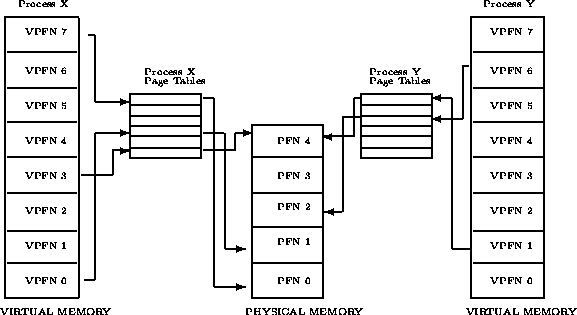
\includegraphics[height=6cm]{pics/img9}
  \end{center}
  \note{Nous verrons  par la suite comment passer  du mode superviseur
    au  mode utilisateur  et vice  versa\\}
  \note{Vérifier  sur wikipedia  ``adresse  virtuelle'' et  ``mémoire
    paginée''}
\end{frame}

\begin{frame}{La MMU}
Concretement:
  \begin{itemize}
    \item Les pages peuvent être de tailles fixe ou variables.
    \item Sous Linux,  afin de simplifier la gestion,  on utilise pour
      la plupart des architectures des pages de 4Kio.
    \item La table de page permet d'obtenir un \emph{Page Frame Number (PFN)}
    \item Le PFN correspond aux bits de poids fort de l'adresse physique
    \item  La table  de page  est décomposée  en plusieur  tables (les
      terme   proviennent   de  l'architecture   Intel   et  se   sont
      généralisés):
      \begin{itemize}
      \item Page Global Directory (PGD)
      \item Page Middle Directory (PMD)
      \item Page Table Entry (PTE)
      \end{itemize}
      \item les tables sont aligné sur des addresse de 4K
      \item  ... Seul  les  bits  de poid  fort  (le \emph{PFN})  sont
        nécessaire pour indiquer l'emplacement de la tbale suivante en
        mémoire
      \item  ... Il  est  possible d'utiliser  les  bit restants  pour
        d'autres usages: validité de l'entrée, etc...
      \item          cf          \file{arch/asm/pgtable.h}          et
        \file{include/linux/mm-types.h}, \c{mm_struct->pgd}
    \end{itemize}
\end{frame}

\begin{frame}{La pagination et la MMU}
  \begin{center}
    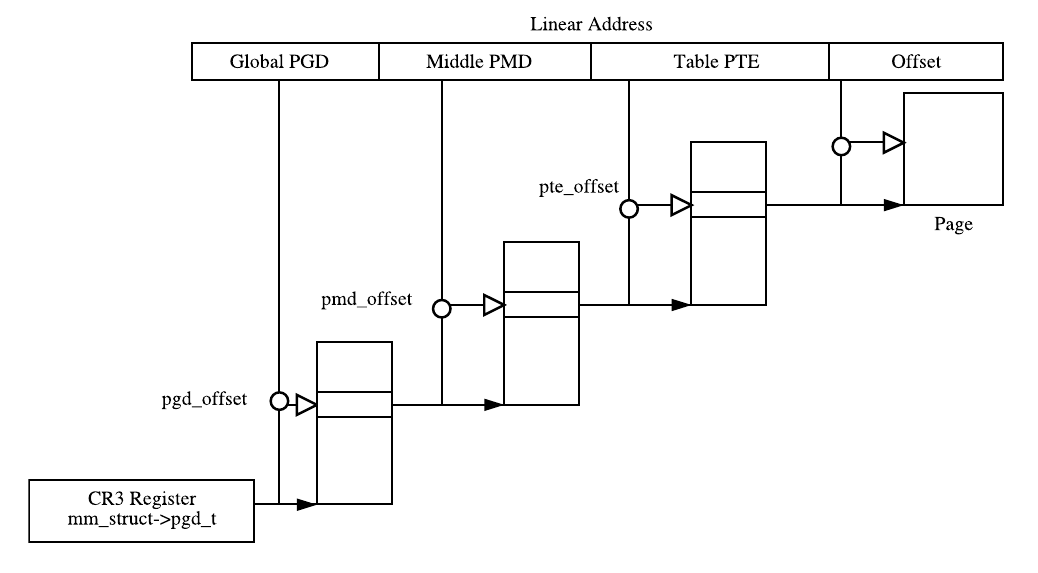
\includegraphics[height=6cm]{pics/linearaddress}
  \end{center}
\end{frame}

\begin{frame}{La MMU - gestion des exceptions}
  Toutes les adresses physiques ne sont pas associées à des adresses
  virtuelles
  \begin{itemize}
  \item Une tâche A ne peut pas accéder à la mémoire d'une tâche B
  \item Protection contre les erreurs de programmation
  \item Permet d'assurer la sécurité des systèmes multi-utilisateurs
  \item Une tâche à l'impression d'avoir toute la mémoire pour elle
  \end{itemize}
\end{frame}

\begin{frame}{La MMU - gestion des exceptions}
  Toutes  les  adresses  virtuelles  ne  sont  pas  associées  à  des
  adresses physiques
  \begin{itemize}
  \item  Lorsqu'une tâche  accède à  une adresse  non  associée.  Une
    exception est déclenchée.  Cela permet à l'OS de reprendre la main
    et de traiter l'erreur (souvent en tuant la tâche fautive)
  \item Lorsqu'une tâche souhaite allouer de la mémoire
    \begin{itemize}
    \item  La tâche demande à l'OS
    \item  L'OS choisi  un (ou  plusieurs) blocs  de  mémoire physique
      libres
    \item L'OS marque le bloc comme appartenant à la tâche
    \item  L'OS choisi un  espace d'adresse  virtuelle où  associer le
      bloc de mémoire
    \item L'OS met à jour la MMU
    \item L'OS retourne l'adresse virtuelle
    \item cf. \man{sbrk(2)} et \man{mmap(2)}
    \end{itemize}
  \end{itemize}
\end{frame}

\subsection{Passage en mode superviseur}

\begin{frame}{Passage en mode superviseur}
  Un processus utilisateur ne peut pas passer en mode superviseur.

  Comment passer en mode superviseur?
  \begin{itemize}
  \item Lorsqu'une interruption/exception est déclenchée
  \end{itemize}

  Comment appeler une fonction du système?
  \begin{itemize}
  \item  Les  tâches ont  besoin  de  faire  des demandes  au  système
    (exemple: allouer de la mémoire)
  \item Ces fonctions système s'appellent des \emph{appels système} ou
    \emph{syscall} (section 2 des pages de man)
  \item  Elles ont  très  peu de  points  communs avec  les appels  de
    fonctions classiques
  \item   Chaque  \emph{syscall}   est   associé  à   un  numéro   (cf
    \file{sys/syscall.h} \file{asm/unistd\_32.h}, \man{syscalls(2)})
  \end{itemize}

\end{frame}

\begin{frame}{Passage en mode superviseur}
  Pour utiliser les \emph{appels systèmes} (cf. \man{syscall(2)}):
  \begin{itemize}
  \item On place les arguments sur la pile
  \item On place le numéro de l'interruption sur la pile
  \item On déclenche une interruption logicielle (\c{int 0x80})
  \item  Le  CPU  passe  en  mode  superviseur  et  appelle  l'ISR  de
    l'interruption
  \item L'OS prend  la main, regarde le premier élément  de la pile et
    appelle la fonction correspondante (\file{asm-generic/unistd.h})
  \end{itemize}
  Il  existe maintenant des  instructions spéciales  sur les  CPU pour
  optimiser    les    \emph{syscall}    (instructions    \c{sysenter},
  \c{sysexit})
\end{frame}

\section{Optimisation possible grâce à la MMU}

\subsection{Les segfaults}

\begin{frame}{Gestion de la mémoire}
  Gestion des droits sur les pages
  \begin{itemize}
  \item    Il    est     possible    d'affecter    des    droits    en
    lecture/écriture/exécution sur les pages gérées par la MMU
  \item Si la tâche essaye d'écrire sur une page contenant des données
    constantes, il s'agit d'un bug et une exception est levée
  \item  On garantie  que  les pages  \emph{read-only}  ne seront  pas
    modifiées
  \item Une page contenant des données constantes (donné ou code) peut
    être mappée dans plusieurs tâches différentes
  \item ... C'est ainsi que plusieurs instance de la même bibliothèque
    ne sont chargées qu'une fois en mémoire
  \item En retirant les droits  en exécution sur les pages de données,
    on améliore la sécurité du système (impossible d'exécuter une page
    contenant des données)
  \item Une  page accessible  en écriture peut  être mappée  dans deux
    tâches afin de leur permettre de partager des données
  \item cf \file{/proc/PID/maps}
  \end{itemize}
\end{frame}

\begin{frame}{Gestion de l'espace d'adressage virtuel}
  Le MMU permet à l'OS de mieux utiliser la mémoire:
  \begin{itemize}
  \item  L'OS peut  donner  des espaces  d'addressage virtuel  contigu
    alors que la mémoire physique est fractionnée
  \item Le système n'alloue jamais la plage $[0, 1024]$
    \begin{itemize}
    \item Cela donne une plage de valeurs spéciales (ex: NULL)
    \item Ainsi, lors du debug, vous êtes certains qu'un pointeur $\in
      [0, 1024]$ est non valide
    \item En dehors des pointeurs,  les nombres que l'on manipule sont
      très  souvent <  1024.   Ce système  nous  permet de  rapidement
      repérer des casts abusifs entre des integers et des pointeurs
    \end{itemize}
  \item ``Sun a inventé le SegFault''
  \end{itemize}
\end{frame}

\begin{frame}[fragile=singleslide]{Context Swap, cache et MMU}
  \begin{itemize}
  \item  Le  MMU est  associé  à  un  cache appelé  TLB  (Translation
    lookaside buffer)
  \item  Lorsqu'une  tache tente  d'accéder  à  une  adresse, le  MMU
    regarde  le TLB,  si il  trouve l'adresse,  elle  est directement
    traduite (\emph{TLB hit})
  \item  Sinon,   il  est  nécessaire   de  traverser  la   table  des
    pages.  Cette  opération  peut   couter  une  centaine  de  cycles
    d'horloge.
  \item Il existe deux mode de fonctionnement du TLB:
    \begin{itemize}
    \item Automatique: Le MMU parcours automatique la table des pages
    \item  Manuel: Une  exception  est déclenchée.   L'OS parcourt  la
      table, met à jour le TLB et rend la main.
    \end{itemize}
  \item Dans  le cas d'un  système multiprocessus, le  mappping change
    lorsque l'on passe d'une tache à l'autre
    \begin{itemize}
    \item  Certains systèmes nécessitent  d'invalider la  totalité du
      TLB
    \item  D'autre permettent  d'associer  un numéro  de  tâche à  une
      entrée  du TLB. Ainsi,  lorsque la  tâche précédente  reprend la
      main, ses entrées dans le TLB sont encore valides
    \end{itemize}
  \end{itemize}
\end{frame}

\subsection{Overcommit}

\begin{frame}{Overcommit}
  Principe de l'overcommit:
  \begin{itemize}
  \item Une tâche demande une allocation
  \item Le système  enregistre la demande dans le  Memory Manager mais
    ne modifie pas le MMU
  \item  Le  système  indique   à  la  tâche  que  l'allocation  s'est
    correctement déroulée
  \item Lorsque la tâche accède à cette page, une exception est levée
  \item Le système reprend la main
  \item Il remarque qu'il avait promis cette page
  \item Il alloue un bloc physique et met à jour la MMU
  \item Il rend la main à la tâche
  \item Tout est transparent pour la tâche
  \end{itemize}
  Voir             \file{/proc/sys/vm/overcommit\_memory}            et
  \file{/proc/sys/vm/overcommit\_memory}
\end{frame}

\subsection{Mapping des fichiers en mémoire}

\begin{frame}{Gestion de la mémoire}
  Simplification des accès au IO
  \begin{itemize}
  \item   La  tâche   demande  de   mapper  un   fichier   en  mémoire
    (\man{mmap(2)})
  \item cf. \file{/proc/*/maps}
  \item  Le système  alloue un  espace d'adressage  virtuel égal  à la
    taille du fichier
  \item Le fichier en lui même n'est pas chargé en mémoire (\emph{lazy
      loading})
  \item Lorsque la  tâche accès à un espace  du fichier, une exception
    est levée et la page  demandée est chargée de manière transparente
    (\emph{on demand paging})
  \item cf. champ RSS de \file{/proc/*/smaps}
  \end{itemize}
\end{frame}

\begin{frame}[fragile=singleslide]{Les pages \emph{dirty}}
  \begin{itemize}
  \item Quelques  soit la demande de l'utilisateur,  le système marque
    les page associés à des fichier comme Read-Only.
  \item  Ainsi, lorsque  la tâche  tente  d'écrire dans  la page,  une
    exception est levée
  \item  La  page est  alors  marquée  \emph{dirty}, les  droits  en
    écriture sont données et le système rend la main
  \item (Le  marquage des page  \emph{Dirty} peut aussi  être effectué
    automatiquement par le CPU)
  \item Le système sait que  cette page devra être synchronisé avec la
    mémoire de masse
  \item Le système peut repousser cette opération
  \item Lorsque  le système  a synchroniser la  page, il la  marque de
    nouveau Read-Only
  \item Lorsque  le système  à besoin de  mémoire, il peut:
    \begin{itemize}
    \item Décharger les page readonly ou les pages \emph{clean}
    \item écrire  les pages  modifiées sur le  disque et  décharger la
      page de la mémoire
    \end{itemize}
  \item cf. champ Dirty de \file{/proc/*/smaps} et \man{free(1)}
  \end{itemize}
\end{frame}

\begin{frame}[fragile=singleslide]{Partage de page}
  \begin{itemize}
  \item Une  tâche peut demander explicitement de  partager un segment
    de mémoire avec une autre page.
  \item Il  suffit de  faire pointer deux  adresse virtuelle  vers la
    même adresse physique
  \item Lorsqu'un fichier (ou une  section du fichier) est déjà chargé
    en  mémoire,  le  système  ne  duplique  pas  la  page.  Elle  est
    automatiquement marqué comme page partagée
  \item Si  une des  tâche tente d'y  accéder en écriture,  le système
    duplique la  page juste  avant l'accès en  écriture (et  marque la
    nouvelle page comme dirty).
  \end{itemize}
\end{frame}

\subsection{La Swap}

\begin{frame}{La swap}
  \begin{itemize}
  \item La  swap est une partie  de la mémoire de  masse utilisée pour
    stockée des données de la mémoire RAM
  \item Utilisation de la Swap:
    \begin{itemize}
    \item Lorsque le système n'a plus assez de mémoire
    \item Il choisit une page physique qu'il copie sur le disque dur
    \item  Il  invalide  la  page  de  la MMU  de  la  (les)  tâche(s)
      concernée(s)
    \item Lorsque la  tâche accède à la page  supprimée, une exception
      est levée
    \item Le système récupère alors la page sur le disque
    \item Le système réécrit la page dans la mémoire physique
    \item  Il associe  l'adresse virtuelle  demandée avec  la nouvelle
      page physique
    \item L'OS rend la main à la tâche
    \item Tout est transparent pour la tâche
    \end{itemize}
  \item Voir \file{/proc/sys/vm/swappiness}
  \end{itemize}
\end{frame}

\begin{frame}[fragile=singleslide]{Compression de la mémoire}
  Compression de la mémoire
  \begin{itemize}
  \item  Mécanisme remplaçant  la  swap sur  les  système dépourvu  de
    mémoire  de   masse  (ou  mémoire  de  masse   limités  en  nombre
    d'écritures)
  \item  Au lieu  de copier  les page  que un  disque, les  pages sont
    compressés
  \item Mis  à part les  heuristiques utilisée, le  fonctionnement est
    identique
  \end{itemize}
\end{frame}

\begin{frame}[fragile=singleslide]{\c{mlock} et \c{mlockall}}
  \begin{itemize}
  \item Les fonctions systèmes \c{mlock} et \c{mlockall} permettent de
    demander à Linux de garder des pages (ou la totalité en mémoire)
  \item Elle empêche ainsi l'utilisation de l'overcommit et du swap.
  \item Il  ne faut  pas oublier d'allouer  une pile  suffisante avant
    d'appeler \c{mlockall} \note{Ajouter du code à ce sujet}
  \end{itemize}
\end{frame}

\begin{frame}[fragile]{Utilisation de \c{mlock}}
\begin{lstlisting}
#include <sys/mman.h>

void alloc_stack_1k() {
  char t[1024];
}

int main() {
  alloc_stack_1k();
  mlockall(MCL_CURRENT | MCL_FUTURE);
}
\end{lstlisting}
\end{frame}

\subsection{Mapping de périphérique en mémoires}

\begin{frame}{Gestion de la mémoire}
  Sécurisation des accès aux périphériques
  \begin{itemize}
  \item  Lorsque  les  registres  des  périphériques  sont  mappés  en
    mémoire, on utilise la MMU pour y accéder
  \item Il  est possible d'autoriser  l'accès à un périphérique  à une
    tâche sans lui donner d'accès au reste du système
  \item Un  système utilisant très fortement cette  méthode est appelé
    micro-kernel
  \item La méthode est peu  utilisée sous Linux (on utilisera \c{mmap}
    sur \file{/dev/mem})
  \item cf. \man{ioperm(2)}
  \end{itemize}
\end{frame}

\begin{frame}[fragile=singleslide]{\emph{mmap} sur des filedevice}
  \begin{itemize}
  \item Il est possible de  mapper en mémoire des fichier périphérique
    (avec \man{mmap(2)})
  \item  L'interprétation  de  cette  de  demande  est  laissée  à  la
    discrétion du driver
  \item Dans certains cas, ca n'a pas de sens: un port série
  \item \file{/dev/mem}:  permet de  mapper toute la  mémoire physique
    sur une adresse virtuelle
  \item  \file{/dev/video0}   (Webcam):  L'espace  de   mémoire  mappé
    représentera une frame.
  \item \file{/dev/fb0} (Frame buffer): L'espace de mémoire représente
    l'écran
  \item Ce mécanisme évite les recopies de données
  \end{itemize}
\end{frame}

\begin{frame}[fragile=singleslide]{Architecture d'un DMA}
  Un DMA \emph{Direct Memory Access}:
  \begin{itemize}
  \item Il s'agit d'un mécanisme matériel.
  \item Il doit être supporté par le contrôleur de mémoire (comprenant
    le MMU), le périphérique (ou le bus) et par l'OS
  \item  Le driver  donne au  périphérique une  adresse  (physique) où
    écrire
  \item Le périphérique demande un canal DMA au contrôleur
  \item Dans le cas d'un  PC, c'est le contrôleur PCI (le northbridge)
    qui joue le rôle de contrôleur
  \item  Le  périphérique écrit/lit  ses  données  en  passant par  le
    contrôleur de mémoire mais sans passer par le CPU
  \item Le périphérique  déclenche une interruption lorsque l'ensemble
    des données sont écrites/lues
  \end{itemize}
  Le  driver peut  décider  de  mapper la  zone  DMA directement  dans
  l'espace d'adressage de la  tâche utilisateur. Avec ce mécanisme, il
  est possible de traiter de grande quantité de données sans copie.
  \note[item]{Ajouter un shéma}
\end{frame}

\begin{frame}[fragile=singleslide]{Fonctionnement    d'un    récepteur
    satellite haut de gamme}
  \begin{itemize}
  \item Un  récepteur satellite (ou IP-TV)  est principalement composé
    d'un démodulateur/démultiplexeur et d'une carte graphique.
  \item Ces deux périphérique sont équipés de DMA
  \item  On  alloue  une  zone  de mémoire  suffisamment  grande  pour
    réceptionner quelques images (2 - 3 au moins)
  \item L'OS passe l'adresse de cette zone au démultiplexeur
  \item Des que le multiplexer à fini d'écrire une frame, il déclenche
    une interruption (et  continue d'écrire la suite dans  la suite du
    DMA)
  \item L'OS  reprend la main. Il  passe l'adresse de cette  zone à la
    carte graphique.
  \end{itemize}
  Il est ainsi possible de transférer de grande quantité de données en
  limitant l'utilisation  du CPU (et  les risque de problème  de temps
  réel)
\end{frame}

\section{Threads et Processus}

\begin{frame}{Threads}
  Thread versus Processus
  \begin{itemize}
  \item On appelle les  tâches ayant des contextes mémoires différents
    des \emph{Processus} (cf. \man{fork(2)})
  \item  Il est  possible  d'exécuter plusieurs  tâches  dans un  même
    contexte mémoire
  \item  Ces  tâche sont  appelées  \emph{threads} ou  \emph{processus
      légers} (cf. \man{clone(2)})
  \item Le fonctionnement  est alors identique au mode  sans MMU, avec
    les mêmes défauts et avantages:
    \begin{itemize}
    \item Pas  de protection contre  les erreurs de  programmation des
      autres threads
    \item Partage de l'information simplifiée
    \item Passage d'une thread à une autre beaucoup plus rapide
    \end{itemize}
  \end{itemize}
  \note{Attention au latence lors de l'allocation, et du swap}
\end{frame}

\begin{frame}[fragile]{Utilisation de processus}
\begin{lstlisting}
#include <unistd.h>

int main() {
  int r;

  r = fork();
  if (r < 0) {
     // Error
  } else if (r > 0) {
    // Parent
  } else /* r == 0 */ {
    // Child
  }
}
\end{lstlisting}
\end{frame}

\begin{frame}[fragile]{Utilisation de threads}
\begin{lstlisting}
#include <pthread.h>

void *task(void *arg) {
  int val = (int) arg;
  // Child
}

int main() {
  int arg = 42
  pthread_t id;
  pthread_create(&id, NULL, task, (void *) arg);
  // Parent
}
\end{lstlisting}
\end{frame}

\subsection{Gestion par l'OS}

\begin{frame}[fragile]{Mapping de l'OS}
  \begin{itemize}
  \item  Une  interruption  peut  avoir  lieu  depuis  n'importe  quel
    processus
  \item Lors d'une interruption (ou  d'un appel système), le CPU passe
    en mode  superviseur, mais  le mapping mémoire  reste celui  de la
    tâche d'origine
  \item Pour  des raison de performance,  il est préférable  de ne pas
    faire  de  changement de  mapping  durant  l'éxecution de  l'appel
    système (ou de l'interruption)
  \item Le noyau se trouve donc  dans une zone interdite en accès mais
    toujours mappé au même endroit quelquesoit la tâche.
  \item Afin  de simplifier les opérations  d'acces aux entrée/sortie,
    le  mapping du  noyau est  dit 'flat  mapping'. C'est  à  dire que
    chaque addresse  virtuelle correspond à une adresse  physique + un
    offset constant  (par défaut sur PC: \c{0xC0000000},  c'est à dire
    3Go). Cet espace s'apelle \emph{low memory}
  \end{itemize}
\end{frame}

\begin{frame}[fragile]{Mapping de l'OS}
  \begin{itemize}
  \item Le noyau peut allouer de  la mémoire en dehors de la \emph{low
      memory} (en \emph{high memory}),  mais il devrat peut-être faire
    un changement de mapping mémoire pour y accéder.
  \item  Le noyau  réserve la  \emph{low memory}  pour son  usage. Une
    tache ne peut pas allouer de la mémoire dans cette zone.
  \item Par défaut sur Linux 32bits, l'espace est partagé en 1Go / 3Go
    (Windows: 2Go / 2Go)
  \item Sur un système possédant  moins de 1Go de mémoire physique, le
    kernel  peut accéder  à  tout  l'espace physique  à  partir de  la
    \emph{low  memory}.  Sinon,  il peut  potentiellement y  avoir des
    pertes de performances  lors de l'accès par le  noyau à la mémoire
    physique supérieure au premier Gigaoctet.
  \item Une application demandant  plus de 3Go d'espace virtuelle peut
    ne pas fonctionner
  \item La solution: passer en 64bits.
  \end{itemize}
\end{frame}

\note{Montrer l'arborescence du kernel: mm, kernel, include, arch, drivers, scripts, tools, Documentation, }

  % Algorithme de gestion de la mémoire
  % Les IPC: Bus logiciel, etc...
%
% This document is available under the Creative Commons Attribution-ShareAlike
% License; additional terms may apply. See
%   * http://creativecommons.org/licenses/by-sa/3.0/
%   * http://creativecommons.org/licenses/by-sa/3.0/legalcode
%
% Copyright 2010 Jérôme Pouiller <jezz@sysmic.org>
%

\part{Gestion de la mémoire utilisateur}

\begin{frame}
  \partpage
\end{frame}

\begin{frame}
  \tableofcontents[currentpart]
\end{frame}

\section{Les différents type de mémoire}

\subsection{Les différents segments}

\begin{frame}[fragile=singleslide]{Différents segments}
  \begin{itemize}
  \item \c{.text}: Code \c{r-x}
  \item \c{.data}: Variables globales (et statiques) \c{rw-}
  \item \c{.bss}: Variables globales initialisées à zéro \c{rw-}
  \item \c{.rodata}: Variables globales constantes \c{r--}
  \end{itemize}
  cf. \cmd{objdump -h}
\end{frame}

\subsection{La pile}

\begin{frame}[fragile=singleslide]{La pile}
  \begin{columns}
    \begin{column}{6.5cm}
      \begin{itemize}
      \item Permet d'allouer les variable \emph{auto}.
      \item = Variable locales au fonction
      \item La pile système est composée de \emph{frame}
      \item Chaque appel de fonction ajoute une \emph{frame} à la pile
      \item Deux registres sont utilisé pour la pile:
        \begin{itemize}
        \item Stack Pointer (\c{$sp}): Pointe la tête de la pile
        \item  Frame Pointer  (\c{$fp})  ou Base  stack Pointer  (\c{$bp}):
          Pointe sur (plus ou moins) la base de la frame en cours
        \end{itemize}
      \item On  accède à un variable  locale en lisant  l'adresse \c{$fp + #CONSTANTE}
      \end{itemize}
    \end{column}
    \begin{column}{4cm}
      \pgfimage[width=5cm]{pics/fig3}
    \end{column}
  \end{columns}
\end{frame}

\begin{frame}{La pile}
  \begin{columns}
    \begin{column}{4cm}
      \begin{itemize}
      \item  Lorsque l'on appel  une fonction,  on sauvegarde  le contexte
        (dont \c{$sp}) à  partir de \c{$sp}, on affecte  \c{$sp} à \c{$fp}
        et on  ajoute la somme de  la taille du contexte  et des variables
        allouées localement à \c{$sp}
      \item Ainsi une allocation locale est très rapide (incrémentation de
        \c{$sp})
      \end{itemize}
    \end{column}
    \begin{column}{6.5cm}
      \begin{overprint}
        \onslide<1>

        \onslide<2>
        \pgfimage[width=7cm]{pics/fig3}

        \onslide<3>
        \pgfimage[width=7cm]{pics/fig4}

        \onslide<4>
        \pgfimage[width=7cm]{pics/fig5}
      \end{overprint}
    \end{column}
  \end{columns}
\end{frame}

  % $sp = $fp
  % $fp = *$fp
  % jmp $sp

  % Sans $fp:
  % $sp = $sp - #FRAME_SIZE
  % jmp $sp

\begin{frame}[fragile=singleslide]{Allocation dynamique sur la pile}
  \begin{itemize}
  \item   Les   fonctions   avec   un  nombre   variable   d'arguments
    (\emph{variadic functions}, cf  \man{va\_arg(3)}) ont une taille de
    frame variable en fonction du nombre d'arguments.
  \item  Il  est  possible   d'allouer  dynmaiquement  de  la  mémoire
    supplémentaire sur la frame courante: \man{alloca(3)}
  \item C'est ainsi que sont implémentés des choses du genre
    \begin{lstlisting}
void f(int i) {
   char t[i];
}
    \end{lstlisting}
  \end{itemize}
\end{frame}

\begin{frame}[fragile=singleslide]{\c{omit-frame-pointer}}
  \begin{itemize}
  \item Durant la compilation \cmd{gcc} connait la taille de la frame
  \item Il est  possible de travailler avec \c{$sp}  comme base plutôt
     que \c{$fp}.
    \begin{itemize}
    \item     Au     retour     de     la    fonction,     on     fait
      \c{$sp = $sp - #SIZE_FRAME} au lieu de \c{$sp = $fp}
    \item Cela permet d'économiser un registre
    \item  Permet d'avoir  du code  un peu  plus rapide  en  gérant un
      registre de moins
    \item   Plus   difficile    à   implémenter   car   \c{$sp}   peut
      potentiellement varier
    \item Option \cmd{-fomit-frame-pointer}
    \item Lors  de l'éxecution,  les outils extérieur  (debuggueur) ne
      connaissent  pas la  taille de  la  frame. Ils  ne peuvent  plus
      retrouver  la  base de  la  frame  et  auront des  difficulté  à
      fonctionner.
    \item Depuis la version  6, \c{gdb} possède quelques contournement
      pour deviner la structure de  la pile, mais ca ne fonctionne pas
      toujours.
      \note[item]{Exemple de gdb avec \cmd{-fomit-frame-pointer}}
    \end{itemize}
   \end{itemize}
\end{frame}

\subsection{Le tas}

\begin{frame}[fragile=singleslide]{Le tas}
  \begin{itemize}
  \item Mémoire utilisée par malloc ou new.
  \item  Les  demande  au  Noyau  se font  par  \man{sbrk(2)}  ou  par
    \man{mmap(2)} pour les demandes supérieures ou égale à une page.
  \item malloc ne peut pas utiliser  mmap pour de petits objets car il
    y aurait trop de perte.
  \item  Lors  d'une demande  d'allocation,  \c{malloc} recherche  une
    place dans les pages qu'il a  deja alloué. Si ca n'est pas le cas,
    il appelle \c{sbrk} ou \c{mmap}
  \item malloc ajoute au début  (ou éventuellement à la fin) des blocs
    alloués des information sur la taille du bloc, etc...
  \item Plusieurs algorithme de gestion de \c{malloc}
  \end{itemize}
\end{frame}

\begin{frame}{Liste de blocs}
  Les  liste  de   bloc:  on  utilise  une  liste   chainée  de  blocs
  libre. Lorsqu'on  libére un  bloc, on vérifie  si les  blocs voisins
  sont libres.  On les fusionne si c'était le cas.
  \begin{center}
    \pgfimage[width=10cm]{pics/alloc-freelist}
  \end{center}
  Problème inhérant à cet algorithme: la fragmentation
  \\[2ex]
  Lors  de l'allocation, quatres méthodes.
\end{frame}

\begin{frame}{Liste de blocs}
  \emph{First fit}  On utilise  le premier bloc  assez grand  que l'on
  trouve
  \\
  Exemple (\textbf{A}jout, \textbf{D}elete):
  \begin{center}
    \pgfimage[width=10cm]{pics/alloc-firstfit}
  \end{center}
\end{frame}

\begin{frame}{Liste de blocs}
  \emph{Next  fit} Idem  \emph{First  fit}, mais  on  part du  dernier
  endroit ou a alloué
  \\
  Exemple (\textbf{A}jout, \textbf{D}elete):
  \begin{center}
    \pgfimage[width=10cm]{pics/alloc-nextfit}
  \end{center}
\end{frame}

\begin{frame}{Liste de blocs}
  \emph{Best fit}  On recherche le  bloc disponible de taille  la plus
  proche de  celle nécessaire.  Il s'avère que  cette méthode garantie
  que l'espace inutilisé est petit et donc inutilisable
  \\
  Exemple (\textbf{A}jout, \textbf{D}elete):
  \begin{center}
    \pgfimage[width=10cm]{pics/alloc-bestfit}
  \end{center}
\end{frame}

\begin{frame}{Liste de blocs}
  \emph{Worst  fit}   Utilise  le   plus  gros  bloc   disponible.  En
  comparaison de  \emph{Best fit}, il  ne permet pas d'avoir  des gros
  bloc  aussi important,  en revanche,  il limite  la perte  des petit
  espace.  Paradoxalement, c'est plutot une bonne stratégie.
  \\
  Exemple (\textbf{A}jout, \textbf{D}elete):
  \begin{center}
    \pgfimage[width=10cm]{pics/alloc-worstfit}
  \end{center}
   Problème inhérant à cet algorithme: la fragmentation
\end{frame}

\begin{frame}[fragile=singleslide]{Allocation binomiale}
  Allocation binômiale (buddy system)
  \begin{itemize}
  \item La mémoire disponible est regroupée en bloc de $2^n$ octets
  \item Ainsi, un  bloc d'ordre 2 fait 4 octets,  d'ordre 3, 8 octets,
    etc...
  \item On alloue toujours des bloc d'une taille de puissance de 2
  \item Si  aucun bloc de cette  taille est disponible,  on utilise un
    bloc d'ordre supérieur que l'on divise en deux
  \end{itemize}
  Exemple (\textbf{A}jout, \textbf{D}elete):
  \begin{center}
    \pgfimage[width=8cm]{pics/alloc-buddy}
  \end{center}
\end{frame}

\begin{frame}[fragile=singleslide]{Les pools de mémoires}
  Les pool de mémoires
  \begin{itemize}
  \item  Utilisé dans  les  application allouant  de grandes  quantité
    d'objets identiques
  \item On  crée des pools  de mémoire que  l'on découpe en  espace de
    taille égale
  \item On utilise une simple bitmap pour géré les bloc disponibles
  \item Algorithme le plus rapide et ayant le moins de frgamentation
  \item Principe du slab dans le noyau (\file{/proc/slabinfo})
  \end{itemize}
\end{frame}

\begin{frame}[fragile=singleslide]{\c{brk} vs \c{mmap}}
  Utilisation de \c{brk} ou de \c{mmap}
  \begin{itemize}
  \item \c{brk} garantie  un espace de mémoire continue  ce qui facile
    l'agrandissement
  \item \c{brk} ne permet pas de libérer un bloc au milieu du tas
  \end{itemize}
  Certains algorithme essaie de tirer  profit au maximum de mmap et de
  ne pas allouer de donnée à cheval sur deux pages de mémoires.
\end{frame}

\begin{frame}[fragile=singleslide]{GNU malloc}
  L'implémentation actuelle de  GNU-malloc utilise un mélange de
  ces principes en fontion de la taille du bloc demandé.
  \begin{itemize}
  \item Free-list + Best fit pour les tailles inférieure à 256 octets
  \item buddy-system pour les allocation entre 256o et 256Ko
  \item mmap pour le reste
  \end{itemize}
  %         Reprendre        les        exemples         de        cf:
  % https://umdrive.memphis.edu/blstuart/htdocs/excerpt3.pdf
\end{frame}

\subsection{Détails d'implémentation dans Linux}

\begin{frame}[fragile=singleslide]{Résumé}
  Résumé:
  \begin{itemize}
  \item \emph{File backed memory}
    \begin{itemize}
    \item \c{.text}, \c{.rodata}, \c{.data}
    \item \c{mmap}
    \item Traité comme de la mémoire anonyme si modifié et privée (=Copy-On-Write)
    \end{itemize}
  \item Mémoire anonyme
    \begin{itemize}
    \item \c{.bss}
    \item \c{mmap}
    \item Pile
    \item Tas
    \item Potentielement swapable
    \end{itemize}
  \end{itemize}
\end{frame}

\begin{frame}[fragile=singleslide]{Résumé agencement mémoire}
    \pgfimage[width=8cm]{pics/linuxFlexibleAddressSpaceLayout}
\end{frame}

\begin{frame}[fragile=singleslide]{Fonctionnement Linux}
    \pgfimage[width=8cm]{pics/memoryDescriptorAndMemoryAreas}
\end{frame}

\section{Les garbages collectors}

\subsection{Reference counting}

\begin{frame}[fragile=singleslide]{Reference counters}
 Reference counting
    \begin{itemize}
    \item  Un référence  counter et  un système  qui associe  à chaque
      objet (ou bloc de mémoire) de mémoire un compteur.
    \item Chaque fois que le  pointeur est copié dans une variable, le
      compteur  est incrémenté.  Si la  variable est  écrasée  par une
      nouvelle valeur ou est désallouée, on décrémente le compteur
    \item Si le compteur tombe à zero, on peut désallouer l'objet
    \item  Il est  possible  d'utiliser ce  système  en supplément  de
      l'allocation classique afin de vérifier qu'il n'y a pas d'erreur
      (si  le compteur tombe  à zero,  c'est une  fuite, si  on libère
      alors que le compteur est  supérieur à 1, il y a potentiellement
      un problème)
    \end{itemize}
  \end{frame}

\begin{frame}[fragile=singleslide]{Reference counters}
  Plusieurs manière de l'implémenter:
  \begin{itemize}
  \item En C, on s'interdit les opérateurs d'affectation classiques et
    on  passe  par  des  fonctions qui  effecturons  l'affectation  et
    l'instrumentation.  Très contraingant, difficile de garantir qu'il
    n'y a pas d'autres affectation.  Il n'est pas possible de detecter
    la destruction d'un pointeur qui se trouve sur la pile.
  \item   En  C++,   il   est  possible   de  surcharger   l'opérateur
    d'affectation   pour  rendre  l'opération   transparentes.   Aussi
    appellé   \emph{smart  pointer}   dans   la  literature.    Classe
    \c{shared_ptr}            de            libboost.             (cf.
    \url{http://www.josuttis.com/libbook/cont/countptr.hpp.html})
  \item Dans une  machine virtuelle, ou dans un  langage de script, on
    controle  tous les  accès à  la mémoire,  donc ca  ne pose  pas de
    problème
  \end{itemize}
\end{frame}

\begin{frame}[fragile=singleslide]{Reference counters}
  \emph{Conservative garbage collector}: Il est possible de scanner la
  mémoire  à  la recherche  de  pattern  ressemblant  à des  addresses
  (double mots > 1024).  Il est ainsi possible de retrouver combien de
  pointeur  pointent  sur  chaque  objets. Peuvent  générer  des  faux
  positifs par
  \begin{itemize}
  \item Des pattern qui ressemble à des pointeur
  \item Des pointeurs internes (exemple: heritage d'objets en C++)
  \end{itemize}
  % La  technique  est pas  utilisé comme  garbage
  % collector, mais  plutôt comme outils  d'instrumentation (Dans le
  % noyau Linux: kmemleak)
\end{frame}

\begin{frame}[fragile=singleslide]{Reference counters}
  \begin{itemize}
  \item  Problème 1:  Dans  le cas  de  système multiprocesseurs,  les
    opérations  sur  les pointeur  doivent  être  atomique.  Or  cette
    opértion est relativement lente.
  \item Problème 2: les références circulaires
  \item L'ensemble des objets est un graphe orienté. Il est nécessaire
    de  faire  une  recherche  de  sous-graphe  indépendants.   Si  un
    sousgraphe  n'est référencé  par aucune  variable  globale (.data,
    .rss, etc...) ou locale (pile)
  \item  Il est théoriquement  nécessaire de  faire cette  recherche à
    chaque décrémention  du compteur de référence:  Lent et générateur
    de latence
  \item Lors de la décrémentation  on ajoute l'objet dans la liste des
    objets à vérifier et  on retarde la recherche.
  \end{itemize}
\end{frame}

\begin{frame}[fragile=singleslide]{Reference counters}
  \begin{itemize}
  \item La recherche de sous-graphe se fait alors:
    \begin{itemize}
    \item Lors de l'allocation ou  à un autre moment définit (stop the
      world). Moins de perte de performance, mais toujours problème de
      latence
    \item  Dans  une  thread  séparée  (concurent).   Peut  créer  des
      problème  d'accès concurrents.  Par  forcement possible  sur les
      petit systèmes
    \item Incrémentale,  à chaque déréférencement ou  à chaque période
      de temps fixe, on parcourt une partie du graphe
    \end{itemize}
  \item On peut ajouter des heuristiques sur les objets à scanner. Par
    exemple: commencer par les objets les plus jeunes qui ont surement
    des  durées de  vie plus  courte  que les  vieux objets  (surement
    présent pour toute la durée du vie du programme).
  \end{itemize}
\end{frame}

\begin{frame}[fragile=singleslide]{Autre technique: \emph{tri-color marking}}
  \begin{itemize}
  \item On  arrête le  fonctionnement du programme  à un  moment donné
    (demande d'allocation supplémentaire, etc...).
  \item On utilise trois marques pour les objets:
    \begin{itemize}
    \item blanc: on ne sait pas si l'objet est référencé
    \item gris: l'objet est référencé, mais on a pas encore scanné ses
      dépendence
    \item noir: référencé et analysé
    \end{itemize}
  \end{itemize}
\end{frame}  

\begin{frame}[fragile=singleslide]{Autre   technique:  \emph{tri-color
      marking}}
  \begin{itemize}
  \item Au départ, tous les objets sont blancs.
  \item  On marque  gris tous  les objet  accéssible depuis  la racine
    (pile, variables globales).
  \item Pour  chaque element de  l'ensemble gris, on grise  les objets
    référencé et on marque l'objet en noir.
  \item On itère jusqu'à ce que l'ensembel gris soit vide
  \item Tous  les éléments restant dans l'ensemble  blanc peuvent être
    désalloués
  \item On reprend le fonctionnement normal du programme.
  \item  Algorithme \emph{stop  the world}.   Difficultés  pour rendre
    l'algorithme itératif
  \item On peut s'appuyer sur certaines assertion de l'algorithme:
    \begin{itemize}
    \item Un objet noir ne pointe jamais sur un blanc
    \item  Les   objet  vont  toujours   de  blanc,  vers   gris  vers
      noir. Jamais l'inverse.
    \end{itemize}
  \end{itemize}
\end{frame}

\section{Technique de debug mémoire}

\begin{frame}[fragile=singleslide]{dmalloc}
  \begin{itemize}
  \item  Enregistre les  bloc alloué  et les  bloc désalloués.  On est
    capbale de lister les blocs non désalloué en sortie de programme
  \item  Ajout de  garde-fou  avant  et après  les  blocs alloués  par
    malloc. Si lors  de la libération les garde-fous  ont été modifié,
    il y a un problème.
  \item  Ecriture   d'un  pattern  sur  la  mémoire   juste  après  sa
    libération. Permet  de garantir que  les donné lues après  un free
    seront corrompue.
  \item Lors de l'allocation, on vérifie que la mémoire a remplie avec
    le pattern. Si ca n'est pas le cas, une violation d'écriture s'est
    produite entre temps.
  \item  Permet aussi  de garantir  que le  code réinitialise  bien la
    mémoire après l'avoir alloué
  \end{itemize}
\end{frame}

\begin{frame}[fragile=singleslide]{dmalloc}
  \begin{itemize} 
  \item Paquet Ubuntu bugué: \url{https://bugs.launchpad.net/ubuntu/+source/dmalloc/+bug/971174}
  %\item \cmd{ wget http://dmalloc.com/releases/dmalloc-5.5.2.tgz}
  %\item \cmd{tar xvzf dmalloc-5.5.2.tgz}
  %\item Suppression des surcharges des fonctions dans \file{malloc.c}
  %\item \cmd{ ./configure && make && sudo make install}
  \item Ajouter \c{#include <dmalloc.h>}
  \begin{lstlisting}
$ gcc -g debug_mem.c -ldmalloc -o debug_mem_dmalloc
$ dmalloc -DV
$ dmalloc -tV
$ dmalloc high -m error-abort -l dmalloc.out
$ echo 123456 | DMALLOC_OPTIONS=debug=0xcb4ed2b,log=dmalloc.out ./debug_mem_dmalloc
$ less dmalloc.out
  \end{lstlisting}
  \end{itemize}
\end{frame}

\begin{frame}[fragile=singleslide]{Libefence, DUMA et kmemcheck}
  \begin{itemize}
  \item Le principe est de s'aider de la MMU pour détecter les erreurs
    d'accès mémoire
  \item  La mémoire est  allouée avec  mmap. On  retire les  droits en
    lecture et en écriture sur le bloc de mémoire alloué.
  \item  A chaque  accès, en  lecture ou  écriture, une  exception est
    déclenché.
  \item Le système récupère la main, log l'accès et vérifie si l'octet
    sur lequel s'effectue l'accès est autorisé
  \item  Permet de détecter  l'erreur dès  qu'elle se  produit (plutot
    qu'à l'allocation suivante)
  \item Permet  de détecter un accès  en lecture sur  une addresse non
    initialisé
  \end{itemize}
\end{frame}

\begin{frame}[fragile=singleslide]{Libefence, DUMA et kmemcheck}
  \begin{lstlisting}
$ gcc -g debug_mem.c -o debug_mem_duma
$ echo 1234 | LD_PRELOAD=/usr/lib/libduma.so.0.0.0 DUMA_FILL=1 DUMA_PROTECT_FREE=1 ./debug_mem_duma
$ gdb -core core debug_mem_duma
  \end{lstlisting}
\end{frame}

\begin{frame}[fragile=singleslide]{Valgrind, kmemleak, Mudflap}
  \begin{itemize}
  \item  Utiliser  un  garbage  collector comme  instrumentation  pour
    vérifier la bonne utilisation de la mémoire
  \item Les différents algorithme de garbage collections s'appliquent
  \item   Kmemcheck:  Instrumentation   avec  un   garbage  collecteur
    conservatif dans le noyau
  \item Valgrind: Machine virtuelle JIT natif/natif
    \begin{itemize}
    \item  Permet   d'instrumenter  tous  les  accès   à  la  mémoire:
      referencement, lecture et ecriture
    \item Permet  de repérer  les fuites ET  les mauvais  accès (comme
      DUMA)
    \item La detection de fuites ou de mauvais accès est immédiate
    \item Plus rapide que DUMA grace à la JIT
    \end{itemize}
  \item Plutôt  que d'instrumenter le code durant  l'éxecution, il est
    possible de l'instrumenter durant la compilation
    \begin{itemize}
    \item Mudflap (compilation avec \cmd{-fmudflap})
    \item Nécessite que toutes les bibliothèques soient instrumentées
    \end{itemize}
  \end{itemize}
\end{frame}

\begin{frame}[fragile=singleslide]{Valgrind}
  \begin{lstlisting}
$ gcc -g debug_mem.c -o debug_mem_valgrind
$ echo 123456 | valgrind --leak-check=yes ./debug_mem_valgrind
  \end{lstlisting}
\end{frame}

\begin{frame}[fragile=singleslide]{Mudflap}
  \begin{lstlisting}
$ sudo apt-get install libmudflap0-4.6-dev
$ gcc -g -fmudflap debug_mem.c -lmudflap  -o debug_mem_mudflap
$ echo 12345 | MUDFLAP_OPTIONS='-help' ./debug_mem_mudflap
$ echo 12345 | MUDFLAP_OPTIONS='-print-leaks -check-initialization' ./debug_mem_mudflap
  \end{lstlisting}
\end{frame}

\section{Communication interprocessus}

\begin{frame}[fragile]{Communication interprocessus}
  Les processus  ayant des espace  mémoire séparés, il  est nécessaire
  d'avoir des systèmes plus évolués pour les faire communiquer:\\
  InterProcessus Communication: IPC.
\end{frame}

\subsection{Mémoire partagée}

\begin{frame}[fragile=singleslide]{La mémoire partagée}
  \begin{itemize}
  \item Utilise  le MMU pour partager  une page de  mémoire entre deux
    processus
  \item dans  cette page de  mémoire, il est possible  d'appliquer les
    mécanisme        de       synchronisation        des       threads
    (\man{pthread\_mutexattr\_getpshared(3)})
  \end{itemize}
\end{frame}

\begin{frame}[fragile]{Mémoire partagée}
  Permet d'implémenter les mécanismes classiques entre processus:
  \begin{itemize}
  \item mutex (réentrant ou non)
  \item rwlock
  \item semaphore
  \item message queues
  \item conditions
  \item barrier/rendez-vous
  \end{itemize}
\end{frame}

\subsection{Cohérence de la mémoire}

\begin{frame}[fragile]{Fonctionnement d'un mutex}
  Nécessite une instruction assembleur  permettant un accès en lecture
  et en écriture  en une instruction: \\
  \texttt{test\_and\_set} affecte le registre d'état en fonction de la
  valeur  du registre  et affecte  la valeur  1 au  registre.  On peut
  développer la fonction \c{lock} à partir de là:
  \begin{lstlisting}
void lock(mutex_t *m) {
  while (test_and_set(m))
    schedule();
}

void unlock(mutex_t *m) {
  m = 0;
  schedule();
}
  \end{lstlisting}
\end{frame}

\begin{frame}[fragile]{Fonctionnement d'un mutex}
  Un peu mieux:
  \begin{lstlisting}
void lock(mutex_t *m) {
  while (test_and_set(m)) {
    this_task.reason = m;
    this_task.state = stop;
    schedule();
  }
}

void unlock(mutex_t *m) {
  m = 0;
  foreach (i in tasks)
    if (i.state == stop && i.reason == m)
      i.state = run;
  schedule();
}
  \end{lstlisting}
\end{frame}

\subsection{Les signaux}

\begin{frame}[fragile=singleslide]{Les signaux}
  \begin{itemize}
  \item Idée issue de l'immitation des interruption sur l'OS
  \item +/- spécifique aux systèmes Posix
  \item L'histoire a rendu l'API un peu bordélique
  \item     \man{sigaction(2)},     \man{signal(7)},    \man{kill(2)},
    \man{kill(1)}, \man{sigqueue(3)}
  \item Il existe 64 signaux sous Linux
  \item Certain  signaux peuvent  être envoyé à  partir de  la console
    (c'est  le   noyau  qui  traduit   les  touches  en   signaux,  cf
    \man{stty(1)})
  \end{itemize}
\end{frame}

\begin{frame}[fragile=singleslide]{Les signaux}
  \begin{itemize}
  \item  Les  signaux  <  32  sont nommés  et  ont  une  signification
    particulière:
    \begin{columns}
      \begin{column}{3cm}
        \begin{itemize}
        \item 1: HUP
        \item 2: INT (\c{^C})
        \item 3: QUIT (\c{^\\})
        \item 4: ILL
        \item 5: TRAP
        \item 6: ABRT
        \item 7: BUS
        \item 8: FPE
        \end{itemize}
      \end{column}
      \begin{column}{3cm}
        \begin{itemize}
        \item 9: KILL
        \item 10: USR1
        \item 11: SEGV
        \item 12: USR2
        \item 13: PIPE
        \item 14: ALRM
        \item 15: TERM
        \item 16: STKFLT
        \end{itemize}
      \end{column}
      \begin{column}{3cm}
        \begin{itemize}
        \item 17: CHLD
        \item 18: CONT
        \item 19: STOP (\c{^Z})
        \item 20: TSTP
        \item 21: TTIN
        \item 22: TTOU
        \item 23: URG
        \item 24: XCPU
        \end{itemize}
      \end{column}
      \begin{column}{3cm}
        \begin{itemize}
        \item 25: XFSZ
        \item 26: VTALRM
        \item 27: PROF
        \item 28: WINCH
        \item 29: POLL
        \item 30: PWR
        \item 31: SYS
        \end{itemize}
      \end{column}
    \end{columns}
    \vspace{2ex}
  \item Il existe  un comportement par défaut pour  chaque signal (fin
    de la tâche, suspension, coredump, ignore)
  \item Il  est possible d'associer ces propres  fonctions aux signaux
    (sauf quelques uns)
  \end{itemize}
\end{frame}

\begin{frame}[fragile=singleslide]{Signaux Temps Réels}
\begin{itemize}
\item Les signaux > 32 sont dit \emph{temps-réel}.
    \begin{itemize}
    \item Plusieurs signaux RT peuvent être en attente
    \item Garantie que les signaux arrivent dans l'ordre dans lesquels
      ils ont été envoyés
    \item Possibilité de passer des valeurs en arguments
    \end{itemize}
  \item Tombent en désuétude. Remplacés par des \emph{file descriptor}:
    \begin{itemize}
    \item \man{signalfd(2)}
    \item \man{eventfd(2)}
    \item \man{timerfd\_create(2)}
    \item \man{inotify(7)}
    \end{itemize}
  \end{itemize}
\end{frame}

\subsection{Les bus logiciels}

\begin{frame}[fragile=singleslide]{Les sockets}
  \begin{itemize}
  \item Généralisation des communications réseaux
  \item Système assez ancien
  \item Mécanisme client/serveur
  \item Le serveur ouvre une socket en écoute
  \item Le client se connecte sur le serveur
  \item  La communication  est  assurée par  des \emph{file  descriptor}
    (\c{read}, \c{write}, etc...)
  \item  Il est  possible  de d'associer  la  socket à  un fichier  (ex:
    \file{/tmp/.X11-unix/X0})
  \end{itemize}
\end{frame}

\begin{frame}[fragile=singleslide]{Les bus logiciels}
  \begin{itemize}
    \item Les socket sont puissants mais manquent d'abstraction
    \item Les \emph{Bus logiciels} offrent les abstraction nécessaires
      \begin{itemize}
        \item Broadcasting d'évènement
        \item Souscription à des évènements/filtrage
        \item Possibilité de passer  des structure complexes comme des
          listes de tailles variables ou des attribut optionnels
        \item   Possibilité   d'interroger   un   processus   distant:
          \emph{Remote Procedure Call (RPC)}
        \end{itemize}
      \item Certains bus peuvent fonctionner à travers un réseau
        \item Certains bus s'appuie sur http et/ou xml
  \end{itemize}
\end{frame}

\begin{frame}[fragile=singleslide]{Les RPC}
  Exemples:
  \begin{itemize}
  \item xml-rpc, soap
  \item corba, dcop, dbus
  \item OLE, COM, DCOM
  \item ømq
  \end{itemize}
\end{frame}

  % Fonctionnement des drivers: Char dev, etc... ?
%\include{drivers1}
  % Monolithique/micro, archi Linux, serveurs, bibliothèque, etc...
\part{Architectures des OS}

\begin{frame}
\partpage
\end{frame}

\begin{frame}
\tableofcontents[currentpart]
\end{frame}
\section{Les architectures standard}

\begin{frame}[fragile=singleslide]{Qu'est-ce qu'un noyau?}
  Un ensemble de services nécessitant une gestion centralisée
  \begin{itemize} 
  \item Ordonnanceur
  \item Gestionnaire de mémoire
  \item Drivers
  \item La gestion de  certains service nécessitant d'être centralisé:
    Réseau, les cache de disques, affichage vidéo
  \item  Les API  permettant  de communiquer  avec l'ordonnanceur,  le
    gestionnaire de mémoire (IPC, etc...) et les drivers
  \end{itemize} 
\end{frame} 

\begin{frame}[fragile=singleslide]{Qu'est-ce qu'un OS}
  Caractéristiques similaires au noyau (ordonnanceur, API, etc..) mais
  regroupe :
  \begin{itemize} 
  \item Les services fournis par le noyau
  \item Les  services fournis par des programmes  et des bibliothèques
    extérieures
  \end{itemize} 
\end{frame}

\begin{frame}{Composants de Linux}
  GNU/Linux est finalement un aggloméra:
  \\[2ex]
  \begin{center}
    \begin{tikzpicture}
      \filldraw[cbrown]
       (-0.05,0.95) -- +(9,0) -- +(9,1) -- +(8,1) -- +(8,2) -- +(7,2) -- +(7,3) 
       -- +(6,3) -- +(6,4) -- +(2,4) -- +(2,3) -- +(1,3) -- +(1,1) -- +(+0,1) -- cycle;
% node {Posix};
     \filldraw[ccyan]
       (7,5) -- +(1,0) -- +(1,-1) -- +(1.9,-1) -- +(1.9,0.9) -- +(0,0.9) -- cycle +(1,.5) node {App};
     \filldraw[ccyan]
       (1,5) rectangle +(1.9,0.9) +(1,.5) node {App};
     \filldraw[ccyan]
       (6,4) rectangle +(1.9,0.9) +(1,.5) node {App};
     \filldraw[cyellow]
       (4,4) rectangle +(1.9,0.9) +(1,.5) node {GNU App};
     \filldraw[cyellow]
       (2,4) rectangle +(1.9,0.9) +(1,.5) node {Bash};
     \filldraw[ccyan]
       (1.9,4) -- +(-1,0) -- +(-1,-2) -- +(-1.9,-2) -- +(-1.9,0.9) -- +(0,0.9) -- cycle +(-1,.5) node {App};
     %\filldraw[cyellow]
     %  (0,4) rectangle +(1.9,0.9) +(1,.5) node {App};
     \filldraw[cblue]
       (7,3) -- +(1,0) -- +(1,-1) -- +(1.9,-1) -- +(1.9,0.9) -- +(0,0.9) -- cycle +(1,.5) node {Lib};
     \filldraw[corange]
       (3,3) rectangle +(3.9,0.9) +(2,.5) node {GNU lib};
     \filldraw[corange]
       (1,2) -- +(6.9,0) -- +(6.9,0.9) -- +(1.9,0.9) -- +(1.9,1.9) -- +(0,1.9) -- cycle +(3.5,.5) node {GNU libc};
     \filldraw[cred]
       (0,1) rectangle +(8.9,0.9) +(4.5,.5) node {Noyau Linux};
     \filldraw[cgreen]
       (0,0) rectangle +(8.9,0.9) +(4.5,.5) node {Matériel};
    \end{tikzpicture}
  \end{center}
\end{frame}


\begin{frame}[fragile=singleslide]{Différents types d'architectures}
  On distingue alors:
  \begin{itemize} 
  \item  Les noyaux monolithiques.  Les drivers  et les  services sont
    gérés  dans un  même espace  mémoire.  Tous les  service du  noyau
    s'éxecute en superviseur.
  \item Les  micro-noyaux. Les drivers  et service s'éxecute  dans des
    contextes mémoire différents avec des accès restreints au système.
  \end{itemize} 
\end{frame}

\begin{frame}[fragile=singleslide]{Différents types d'architectures}
  Quelques remarques:
  \begin{itemize} 
  \item   Les  micro-noyaux   sont  plus   robustes  aux   erreurs  de
    développement des drivers
  \item Les micro-noyau possèdent peu d'appels systèmes
  \item  Les  noyau  monolithiques  sont  moins  lourds  en  terme  de
    transfert d'informations
  \item Les micro-noyau sont  plus complexe à architecturer. Tellement
    complexes  qu'il  n'existe pas  d'exemple  de micro-noyau  s'étant
    développé sur des architecture riches
  \end{itemize} 
\end{frame}


\begin{frame}[fragile=singleslide]{Différents types d'architectures}
  \begin{itemize} 
  \item XNU  (le noyau de MacOSX)  est un noyau  monolithique basé sur
    Mach 3 (monolithique aussi)
  \item Hurd, Beos et Mach 4, sont des micro-noyau (peu connus)
  \item Les  hyperviseurs tels  que Adeos ou  VMWare ESX  peuvent être
    apparenté à des micro-noyau (mais pas complètement)
  \item  Windows est  un  noyau hybride.  Windows exporte  suffisament
    d'API  pour  développer des  driver  à  l'extérieur  du noyau  (en
    partiulier les driver USB),  mais les drivers principaux sont dans
    le noyau (graphique, son, etc...)
  \item Linux est un noyau monolithique modulaire.
    \begin{itemize} 
    \item Débat Tanenbaum–Torvalds
    \item \url{http://groups.google.com/group/comp.os.minix/browse_thread/thread/c25870d7a41696d2}
    \item Modulaire depuis  la  version  2.6
    \end{itemize} 
  \item  Linux  permet  de  développer  certains types  de  drivers  à
    l'extérieur du noyau, mais ca  n'est pas son objectif et il montre
    rapidement ses limitations dans  le domaine (Serveur X, Fuse, UIO,
    CUPS, sane, libusb, etc...).
\end{itemize} 

\end{frame} 

% Environs 10 slides -> 30min

% Composition d'un OS multitache
%   Scheduler
%   Gestionnaire de mémoire
%   Des drivers
%   Une API et des services necessitant un "chef d'orchestre": IPC, réseaux, filesystèmes

% Petite partie, a placer avec la virtualisation?
% Noyau monolithique
%   .... mais modulaire
% Micronoyau
% Kernel Hybride
% Hyperviseurs
% Choix des méacanise de communication noyau/user et user/user
% 
% Divrsité de l'API
%   Nombre d'appels système: qqs uns comme Hurd, ou beaucoup comme Linux
%   API stable et definie (Linux) vs API movante (Windows)
%   "Schema de Linux" -> "Linux ne designe que le noyau, etc..."

%\section{La virtualisation}

  % Systèmes de compilation: Make, autotools, cmake
%
% This document is available under the Creative Commons Attribution-ShareAlike
% License; additional terms may apply. See
%   * http://creativecommons.org/licenses/by-sa/3.0/
%   * http://creativecommons.org/licenses/by-sa/3.0/legalcode
%
% Created: 2012-07-28 20:09:12+02:00
% Main authors:
%     - Jérôme Pouiller <jezz@sysmic.org>
%

\section{La compilation}

\subsection{Exemple}

\begin{frame}[fragile=singleslide]{Notre premier programme}{\file{hello.c}}
  \embedfile{samples/hello/hello.c}
  \lstinputlisting[language=c,lastline=15]{samples/hello/hello.c}
\end{frame}

\begin{frame}[fragile=singleslide]{Notre premier programme}{\file{hello.c}}
  \lstinputlisting[language=c,firstline=16]{samples/hello/hello.c}
\end{frame}

\begin{frame}[fragile=singleslide]{Notre premier programme}{\file{hello.h}}
  \embedfile{samples/hello/hello.h}
  \lstinputlisting[language=c]{samples/hello/hello.h}
\end{frame}

\begin{frame}[fragile=singleslide]{Compilation}
  Compilation normale:
  \begin{lstlisting}
host$ gcc -c hello.c -o hello.o
host$ gcc hello.o -o hello
host$ ./hello 1
Hello World
  \end{lstlisting} %$
\end{frame}

\subsection{Fonctionnement de la compilation}

\begin{frame}[fragile=singleslide]{ Le format ELF}
  \begin{itemize} 
  \item La  plupart des fichiers  manipulés par le compilateur  et les
    outils associés sont au format ELF
  \item Ce format est une serie de sections et de tables
  \item  Certaines sections section seront chargée en mémoires
  \item  Certaines  section  demande  à etre  simplement  allouées  en
    mémoire
  \item  \emph{objdump(1)} permet  d'obtenir des  informations  que un
    fichier ELF
  \item  \emph{objcopy(1)}  permet   d'extraire  des  sections  ou  de
    modifier un fichier au format ELF
  \item \emph{readelf(1)}  et \emph{nm(1)}, mais  \c{objdump} contient
    toute leur fonctionnalités
  \end{itemize} 
  La compilation:
  \begin{itemize} 
  \item  Execute  le  préprocesseur  (fichier \c{.i})  Le  compilateur
    vérifie  la syntaxe,  le typage,  converti le  code  en assembleur
    (fichier \c{.s}) puis en code objet (fichier \c{.o})
  \item L'option \c{-c} est utilisé.
  \item Le compilateur doit connaitre les signature des fonction (afin
    de vérifier correctement le typage).
  \item Les  fichiers header  (fichiers \c{.h}) sont  nécessaires pour
    cette phase
  \item  \c{-I} permet  de  spécifier des  chemins supplémentaires  où
    rechercher des fichiers headers (par défaut: \c{/usr/include})
  \item Si un fichier est  inclu entre double-quotes, il est recherché
    dans le même répertoire que le source.
  \item \c{-Wall}, \c{-Wextra} recommandés
  \item \c{-DMACRO} peut etre utilisé
  \end{itemize}
\end{frame} 

\begin{frame}[fragile=singleslide]{Les symboles de debug}
  \begin{itemize}
  \item \c{-g} permet d'ajouter  une section contenant des symboles de
    debug.
  \item  Utilisé  spar les  debuggueur  pour  donner des  informations
    supplémentaire ou pour faire le lien avec les sources.
  \item Cette section n'est pas chargée en mémoire. 
  \item Le format utilisé s'apeller \emph{dwarf} (Debug with Arbitrary
    Record Format).
  \item L'option -g ne change pas le code généré:
    \begin{lstlisting}
$ gcc -g -c main.c -o main-dbg.o
$ gcc -c main.c -o main-rel.o
$ ls -l
-rw-rw-r-- 1 jezz jezz    2125 Aug  3 16:05 main-rel.o
-rw-rw-r-- 1 jezz jezz    3720 Aug  3 16:05 main-dbg.o
$ strip *.o
$ ls -l
-rw-rw-r-- 1 jezz jezz    2096 Aug  3 16:05 main-rel.o
-rw-rw-r-- 1 jezz jezz    2096 Aug  3 16:05 main-dbg.o
    \end{lstlisting} 
  \end{itemize}
  Le compilateur peut effectuer quelques optimisations:
  \begin{itemize}  
  \item Les  fonction et les  variables marquées \c{static}  ne seront
    pas exportés, et donc, pas utilisé par les autres fichier objets.
  \item  Le compilateur peut décider d'\emph{inliner} ces fonctions
  \item Si toutes les appels à une fonctions statique ont été inlinés,
    il peut supprimer la fonction du fichier objet.
  \end{itemize} 
\end{frame} 

\begin{frame}[fragile=singleslide]{L'édition de liens}
  \begin{itemize} 
  \item  Le compilo  ne connait  pas  forcement les  addresses des
    fonctions et des variables globale marquées \c{extern}
  \item  Les endroits  ayant  besoin de  ces fonctions/variables  sont
    remplacés par  des 0 et une  entrée est ajoutée dans  la table des
    \emph{relocation} du fichier objet (cf. \c{objdump -R})
  \item On  appelle le \c{linker} (\c{gcc} sans  l'option \c{-c}) pour
    résoudre les symboles
  \item Le linker connait toutes les fonctions, et toutes les table de
    relocation.
  \item Il peut déplacer les  addresses de chargement des fonctions et
    des variables de  manière à les mettre au  plus près des fonctions
    qui  les   appellent  (optimisation  de   l'utilisation  du  cache
    d'instruction)
  \item Une  fois l'agencement des fonctions défini,  le linker résoud
    toutes les entrées des tables de relocations
  \end{itemize}
\end{frame} 

\begin{frame}[fragile=singleslide]{Les bibliothèques}
  \begin{itemize} 
  \item  Afin de  simplifier  le déploiment  des  utilitaires, il  est
    possible  d'empaqueter  un  ensemble  de fichier  objet  dans  une
    bibliothèque dite statique (fichier .a). cf. \emph{ar(1)}.
  \item Dans ce cas, cela ne change rien à la procedure de link
  \item Il  est aussi possible d'utiliser  des biliothèques dynamiques
    (fichier .so). Nous y reviendrons.
  \item L'usage de bibliothèques dynamique permet:
    \begin{itemize} 
    \item de ne charger qu'un  exemplaire de la bibliothèque pour tout
      le système
    \item de simplifier la redistribution du programme
    \item de simplifier les mises à jour de la bibliothèque
    \end{itemize} 
    % A revoir, il faut peut-etre mettre ces trois points autre part
  \item  Il  est  possible  de  spécifier  le  chemin  complet  de  la
    bibliothèque (dynamique ou statique)  ou de laisser le compilateur
    la trouver  automatiquement avec  la syntaxe \c{-lbrary}.  On peut
    dans ce cas lui précisier des chemins supplémentaire ou rechercher
    la bibliothèque avec \c{-L}
  \item  Par  défaut,  le  compilateur  recherchera  les  bibliothèques
    dynamiques, sauf si l'option \c{-static} est utilisée
  \item  Le  linker suit  en  fait  une  des recettes  contenues  dans
    \c{/usr/lib/ldscripts/}  (en  fonction   des  options  passées  au
    linker).   Il   est  possible  de  fabriquer   son  propre  format
    (\c{ld -T}) (utile pour générer des firmwares).
  \item Problème:  les fichiers objets des  bibliothèques statiques et
    dynamique ne se compilent pas  avec les mêmes options et certaines
    architectures ne permettent  pas les bilbiothèques dynamiques.  La
    création  de  bibliothèque portable  peut  devenir  un vrai  casse
    tête. libtool est outil permettant de faciliter ce travail.
  \end{itemize}
\end{frame} 

 \begin{frame}[fragile=singleslide]{  Les bibliothèques dynamiques}
  \begin{itemize} 
  \item Coté bibliothèque:
    \begin{itemize} 
    \item Elle  contient une  table des symboles  exportés et  de leur
      emplacement (dans la table \emph{.dynsym})
    \item A  la construction, elle  doit être linkée  avec \c{-shared}
      pour indiquer que sont  chargement sera différent d'un programme
      standard (principalement, aucune fonction main n'est nécessaire)
    \end{itemize} 
  \item Coté éxecutable:
    \begin{itemize} 
    \item Le linker va ajouter une table d'indirection (la \emph{.got}
      \emph{Global Offset  Table}) pour tous les  symboles se trouvant
      dans des bibliothèques
    \item Le  linker doit passer  par cette indirection  pour appeller
      une fonction exportée par une biliothèque dynamique.
    \item  Il  ne   peut  pas  faire  tenir  ce   morceau  de  code  à
      l'emplacement laissé par le compilateur
    \item Il crée donc un petit morceau de code qu'il placera dans une
      section \emph{Procedure Linkage Table} (\emph{.plt})
    \item Cette procedure permet  simplement de brancher vers la table
      d'indirection.
    \end{itemize} 
  \item A l'éxécution
    \begin{itemize} 
    \item Un interpreteur (normalement \c{/lib/ld.so}) est appellé
    \item il  charge les  bibliothèques nécessaires (inscrites  dans la
      table \emph{.dynamic}) en mémoire
    \item  Il remplit  la GOT  avec  des pointeurs  vers une  fonction
      permettant la résolution du symbole.
    \item  Lorsque  ce symbol  est  appellé  la  première fois,  cette
      fonction est appellée.
    \item La fonction résoud le symbol et place son adresse dans la GOT
    \item Cette méthode s'appelle \emph{lazy resolving}
    \item   Cela  peut   être   désactivé  en   passant  la   variable
      d'environnement \c{LD_BIND_NOW}
    \end{itemize} 
  \item Il est possible de  demander le chargement manuel et dynamique
    des    bibliothèques    et    des    symboles    avec    \c{libdl}
    (\emph{dl\_open(3)}, \emph{dl\_sym(3)})
  \item Afin d'accélérer le  chargement, \c{ld.so} utilise un index de
    bibliothèques présentes  sur le  système.
  \item  Lorsque vous  ajoutez une  bibliothèque, vous  devez appeller
    \emph{ldconfig(1)} pour mettre à jour ce cache.
  \item la variable \c{LD_LIBRARY_PATH}  permet d'ajouter un chemin de
    recherche de biliothèque pour \c{ld.so}.
  \end{itemize} 
\end{frame} 

\begin{frame}[fragile=singleslide]{Utilisation de \c{LD_PRELOAD}}
  \begin{itemize} 
  \item La vaiable d'envionnement \c{LD_PRELOAD} permet de demander le
    chargement d'une bibliothèque avant  les las autres
  \item Les symboles exportées par celle-ci seront prioritaires.
  \item Exemple:
    \begin{lstlisting} 
unsigned int sleep(unsigned int s) {
    static unsigned int (*real_sleep)(unsigned int s) = NULL;

    if (!real_sleep)
        real_sleep = dlsym(RTLD_NEXT, ``sleep'');

    usleep(5);
    return real_sleep(s);
}
    \end{lstlisting}
  \end{itemize} 
\end{frame} 

\begin{frame}[fragile=singleslide]{A qui fournir quoi?}
  \begin{itemize}
  \item La poubelle
    \begin{itemize} 
    \item Les dependance
    \item Les objets (ELF)
    \end{itemize} 
  \item Les sources:
    \begin{itemize} 
    \item Les sources
    \item Les headers
    \item Le système de compilation
    \end{itemize} 
  \item Les developpeurs externes
    \begin{itemize} 
    \item Les headers
    \item Les bibliothèque statique (archve crée avec \emph{ar(2)})
    \end{itemize} 
  \item L'utilisateur final
    \begin{itemize} 
    \item Les bibliothèque dynamique (ELF)
    \item Les binaires (ELF)
    \end{itemize} 
  \end{itemize} 
\end{frame} 

\begin{frame}[fragile=singleslide]{Identifier le résultat}
  Un bon moyen de reconnaitre  les binaires est d'utiliser la commande
  \emph{file(1)}:
  \begin{lstlisting}
host$ file */hello
hello-dyn:        ELF 64-bit LSB executable, x86-64, version 1 (SYSV), dynamically linked (uses shared libs), for GNU/Linux 2.6.15, not stripped
hello-static: ELF 64-bit LSB executable, x86-64, version 1 (GNU/Linux), statically linked, for GNU/Linux 2.6.15, not stripped
/lib/x86_64-linux-gnu/librt-2.15.so: ELF 64-bit LSB shared object, x86-64, version 1 (SYSV), dynamically linked (uses shared libs), for GNU/Linux 2.6.24, stripped
/usr/lib/x86_64-linux-gnu/librt.a: current ar archive
\end{lstlisting} %$
\end{frame}

\begin{frame}[fragile=singleslide]{redistribution et licences}
  \begin{itemize} 
  \item GPL. Est-ce du travail dérivé?
    \begin{itemize} 
    \item Le resultat d'un copier-coller?
    \item Une compilation statique?
    \item Une compilation dynamique?
    \end{itemize} 
  \item LGPL
  \end{itemize} 
\end{frame}


\begin{frame}[fragile=singleslide]{Règle d'or}
  \begin{center}
    \huge{Jamais d'espaces dans les chemins de compilation}
  \end{center}
\end{frame}

\subsection{Un projet base de Makefile}

\begin{frame}[fragile=singleslide]{Créer un projet sans autotools}
  Utiliser au maximum les règles implicites facilite votre travail
\begin{lstlisting}
host$ touch Makefile
host$ make
\end{lstlisting} %$
\end{frame}

\begin{frame}[fragile=singleslide]{Créer un projet sans autotools}
  Utiliser les règles implicites facilite votre travail
  \lstinputlisting{samples/hello/Makefile.1}
  Testons:
\begin{lstlisting}
host$ make CC=arm-linux-gcc CFLAGS=-Wall
\end{lstlisting} %$
\end{frame}

\begin{frame}[fragile=singleslide]{Créer un projet sans autotools}
  \cmd{VPATH} vous permet de géré la compilation \emph{out-of-source}.
  Remarques que pour que \verb+VPATH+ fonctionne correctement, vous devez avoir
  correctement utilisé le quoting pour les directive d'inclusion (\verb+<+ pour
  les entête systèmes et \verb+"+ pour les entêtes du projet)
  % Pas besoin d'ajouter VPATH = . Du coup, c'est la meme chose que Makefile.1
  %\lstinputlisting{samples/hello/Makefile.2}
  Testons:
\begin{lstlisting}
host$ cd build
host$ make -f ../Makefile VPATH=.. CC=arm-linux-gcc 
\end{lstlisting} %$  
\end{frame}

\begin{frame}[fragile=singleslide]{Créer un projet sans autotools}
  \cmd{gcc} peut  générer les dépendances de vos  fichiers.  On génère
  ainsi  des morceaux  de Makefile  que l'on  inclut. Il  ne  faut pas
  oublier   d'ajouter  la  dépendance   entre  \cmd{hello.d}   et  les
  dépendances de \cmd{hello.c}
  \lstinputlisting{samples/hello/Makefile.3}
  \note{ Voir http://www.makelinux.net/make3/make3-CHP-2-SECT-7.html}
\end{frame}

\begin{frame}[fragile=singleslide]{Créer un projet sans autotools}
  Les  Makefile permettent d'utiliser  des fonctions  de substitutions
  qui  peuvent  nous aider  à  rendre  notre  système plus  générique.
  \lstinputlisting{samples/hello/Makefile.4}
\end{frame}

\begin{frame}[fragile=singleslide]{Créer un projet sans autotools}
  Nous pouvons  ajouter des alias  pour nous aider dans  les commandes
  complexes 
  \lstinputlisting[firstline=11]{samples/hello/Makefile.5}
  \note[item]{TODO: Ajouter des \#ifdef CONFIG pour faire dans Kconfig}
  \note[item]{Parler de apt-get source (-b), dpkg -L, dpkg -l, dpkg-buildpackage}
\end{frame}

\subsection{A base d'Autotools}

\begin{frame}[fragile=singleslide]{Historique des Autotools}
  \note[item]{Faire l'historique de configure/Makefile/autotools}
  \begin{enumerate}
  \item Makefile
  \item Makefile + hacks pour effectuer de la configuration
  \item Makefile.in + configure
  \item Makefile.in + configure.ac
  \item Makefile.am + configure.ac
  \end{enumerate}
\end{frame}


\begin{frame}[fragile=singleslide]{Compiler avec autotools}
  \begin{itemize}
  \item C'est le cas le plus courant
  \item Pour une compilation classique:
\begin{lstlisting}
host$ ./configure
host$ make
host% make install
\end{lstlisting} %$
  \item Compilation \emph{out-of-source}. il est nécessaire d'appeller
    le \file{configure} à partir du répertoire de build.
\begin{lstlisting}
host$ mkdir build
host$ cd build
host$ ../configure
host$ make
host% make install
\end{lstlisting} %$
  \end{itemize}
\end{frame}

\begin{frame}[fragile=singleslide]{Compiler avec autotools}
  Obtenir de l'aide:
\begin{lstlisting}
host$ ./configure --help
\end{lstlisting} %$

  Parmis les fichiers générés:
  \begin{itemize}
  \item \file{config.log}  contient la sortie  des opération effectuée
    lors de l'appel de \cmd{./configure}.  En particulier, il contient
    la ligne de commande utilisée. Il est ainsi possible de facilement
    dupliquer la configuration.
\begin{lstlisting}
host$ head config.log
\end{lstlisting} %$
  \item     \cmd{config.status}     permet     de    regénérer     les
    Makefile.  \cmd{config.status} est  automatiquement appellé  si un
    Makefile.am est modifié.
  \end{itemize}
\end{frame}


\begin{frame}[fragile=singleslide]{Créer un projet avec autotools}
  Fonctionnement des autotools:
  \begin{itemize}
  \item Préparation 
\begin{lstlisting}
% apt-get install automake autoconf
\end{lstlisting}
  \item Déclaration de notre programme et de nos sources pour \cmd{automake}
\begin{lstlisting}
$ vim Makefile.am
\end{lstlisting} %$
\begin{lstlisting}
bin_PROGRAMS = hello
hello_SOURCES = hello.c hello.h
\end{lstlisting}
  \item Les \cmd{autotools}  imposent l'existence de certains fichiers
    de documentation
\begin{lstlisting}
$ touch NEWS README AUTHORS ChangeLog
\end{lstlisting} %$
  \end{itemize}
\end{frame}

\begin{frame}[fragile=singleslide]{Créer un projet avec autotools}
  \begin{itemize}
  \item  Création  d'un  template  pour \cmd{autoconf}  contenant  les
    macros utiles pour notre projet
\begin{lstlisting}
$ autoscan
$ mv configure.scan configure.ac
$ rm autoscan.log
$ vim configure.ac
\end{lstlisting}
  \item Personnalisation du résultat
\begin{lstlisting}
...
AC_INIT([hello], [1.0], [bug@sysmic.org])
AM_INIT_AUTOMAKE
...
\end{lstlisting}
  \item      Génération      du      \file{configure}      et      des
    \file{Makefile.in}. C'est cette version qui devrait être livée aux
    packageurs.
\begin{lstlisting}
$ autoreconf -iv
\end{lstlisting} %$
    \note[item]{Bon, pas de TP la dessus, ca pas très utile}
  \end{itemize}
\end{frame}

\begin{frame}[fragile=singleslide]{Créer un projet avec autotools}
  \begin{itemize}
  \item Compilation
\begin{lstlisting}
$ ./configure --help
$ mkdir build
$ cd build
$ ../configure --host=arm-linux --build=i386 --prefix=$(pwd)/../install
$ make
$ make install
\end{lstlisting} %$
  \end{itemize}
\end{frame}

\begin{frame}[fragile=singleslide]{Créer un projet avec autotools}
  La cible \verb+distcheck+ :
  \begin{enumerate}
  \item Recopie les fichiers référencé dans Autotools
  \item Retire les droits en écriture sur les sources
  \item Lance une compilation \emph{out-of-source}
  \item Installe le projet
  \item Lance la suite de test
  \item Lance un distclean
  \item Vérifie que tous les fichiers créés sont effectivement supprimés
  \item Crée une tarball correctement nommée contenant les sources
  \end{enumerate}
\end{frame}

\begin{frame}[fragile=singleslide]{Créer un projet avec autotools}
  Si \cmd{automake}  est appellé avec  \verb+-gnits+, \verb+distcheck+
  effectue des vérification supplémentaires sur la documentation,
  etc... 
  \\[2ex]
  La fonctionnalité \verb+distcheck+ est  le point fort souvent énoncé
  des autotools.
\begin{lstlisting}
$ make distcheck
$ tar tvzf hello-1.0.tar.gz
\end{lstlisting} %$
\end{frame}

%%% A partir de la, je ne sais pas si je le fais

\subsection{A base kmake}

%% A placer apres le système de Makefile?
%% Peut-être ajouter léxemple d'eolane juste avant
\begin{frame}[fragile=singleslide]{Compiler un programme tiers}{Kconfig}
  \begin{itemize}
  \item Système de compilation du noyau
  \item Très bien adapté à la cross-compilation
  \item Pour configurer les options:
    \begin{itemize}    
    \item En ncurses
\begin{lstlisting}
host% apt-get install libncurses5-dev
host$ make ARCH=arm CROSS_COMPILE=arm-linux- menuconfig
\end{lstlisting} %$
    \item En Qt3
\begin{lstlisting}
host% apt-get install libqt3-mt-dev
host$ make ARCH=arm CROSS_COMPILE=arm-linux- xconfig
\end{lstlisting} %$
    \end{itemize}
  \item Ne pas oublier d'installer les headers des bibliothèques
  \end{itemize}
\end{frame}

\begin{frame}[fragile=singleslide]{Compiler un programme tiers}{Kconfig}
  \begin{itemize}
  \item Pour cross-compiler
\begin{lstlisting}
host$ make ARCH=arm CROSS_COMPILE=arm-linux-
\end{lstlisting} %$
  \item Pour compiler \emph{out-of-source}
\begin{lstlisting}
host$ mkdir build
host$ make ARCH=arm CROSS_COMPILE=arm-linux- O=build
\end{lstlisting} %$
  \end{itemize}
\end{frame}

\begin{frame}[fragile=singleslide]{Compiler un programme tiers}{Kconfig}
  Principaux points importants:
  \begin{itemize}
  \item Adapté au environnements embarqué
  \item Adapté aux environnements avec beaucoup de configuration
  \item Initié par le Kernel Linux
  \item  Pas un  système de  compilation réel. Composé de :
    \begin{itemize}
    \item Kconfig, Système de gestion de configuration
    \item  Kmake, règles  Makefile  bien étudiées.  Chaque projet  les
      adapte à ces besoins
    \end{itemize}
  \item Application de la règle: "Pas générique mais simple à hacker"
  \item Dépend principalement de \cmd{gmake}
  \item Mode verbose: \verb+V=1+
  \item Permet d'effectuer des recherche
  \end{itemize}
\end{frame}

\begin{frame}[fragile=singleslide]{Compiler un programme tiers}{Kconfig}
  Test avec busybox:
  \begin{itemize}
  \item Préparation
\begin{lstlisting}
host$ wget http://busybox.net/downloads/busybox-1.18.3.tar.bz2
host$ tar xvjf busybox-1.18.3.tar.bz2
\end{lstlisting} %$
  \item Récupération d'une configuration par défaut
\begin{lstlisting}
host$ make help
host$ make ARCH=arm CROSS_COMPILE=arm-linux- O=build defconfig
\end{lstlisting} %$
  \item Personnalisation de la configuration
\begin{lstlisting}
host% apt-get install libncurses5-dev
host$ make ARCH=arm CROSS_COMPILE=arm-linux- O=build menuconfig
# Supprimer inetd et le support NFS
\end{lstlisting} %$
  \end{itemize}
\end{frame}

\begin{frame}[fragile=singleslide]{Compiler un programme tiers}{Kconfig}
  Test avec busybox:
  \begin{itemize}
  \item Compilation
\begin{lstlisting}
host$ make ARCH=arm CROSS_COMPILE=arm-linux- 
\end{lstlisting} %$
  \item Installation
\begin{lstlisting}
host$ make ARCH=arm CROSS_COMPILE=arm-linux- install
\end{lstlisting} %$
  \end{itemize}
\end{frame}


\subsection{A base de cmake}
Aucune des solution précédante ne fonctionne sur les OS non posix (rappel: Cygwin = Couche posix pour Windows)




  % Boot: A ecrire! : chargement en memoire, bootloader, kernel, head.S, start_kernel (init/main.c), initrd, rootfs (root=, /bin/init, /etc/inittab, /etc/rcS. /etc/init.d(beurk)), initrd (pour les drivers), boot nfs, boot tftp, mtd/jffs2, ubi
%% This document is available under the Creative Commons Attribution-ShareAlike
% License; additional terms may apply. See
%   * http://creativecommons.org/licenses/by-sa/3.0/
%   * http://creativecommons.org/licenses/by-sa/3.0/legalcode
%
% Copyright 2010 Jérôme Pouiller <jezz@sysmic.org>
%

\part{Démarrer}

\begin{frame}
  \partpage
\end{frame}

\begin{frame}
  \tableofcontents
\end{frame}

\section{Le Boot}

\begin{frame}[fragile=singleslide]{Le Boot}
  Les Bootloaders:
  \begin{itemize}
  \item Le CPU commence par  executer des instructions situées sur une
    addresse mémoire.
  \item  Le  premier  morceau  de  code se  trouve  forcément  mappé
    directement en mémoire
  \item Il  s'agit généralement d'une eeprom ou  d'une rom (Celle-ci
    est directement  mappée sur  le bus d'adresse,  contrairement au
    flash)
  \item   De    nos   jours   les    micro-controlleur   intègre   des
    \emph{bootloader} en ROM
  \item   Ces   bootloader   peuvent   peuvent  avoir   de   nombreuse
    fonctionnalités
  \item Les ROM ont  généralement une capacité limitée (entre quelques
    Ko et quelques Mo)
  \end{itemize}
\end{frame}

\begin{frame}[fragile=singleslide]{Le Boot}
  \begin{itemize} 
  \item L'objectif du premier étage est de charger la suite du système
    en mémoire
    \begin{itemize}
    \item Initialiser un périphérique plus important comme une flash
    \item Copier le contenu du périphérique en mémoire
    \item Sauter sur le bootloader de niveau suivant
    \end{itemize}
  \item Il existe souvent plusieurs étage de bootloader
  \item A la  fin de l'éxecution des bootloaders,  le noyau du système
    d'exploitation doit être présent en mémoire.
  \end{itemize}
\end{frame}

\begin{frame}[fragile=singleslide]{Le Boot}
  Le noyau:
  \begin{itemize}
  \item Généralement compressé.
  \item Le  noyau contient un  bootloader qui décompresse le  noyau en
    mémoire
  \item       Démarrage       de       Linux      proprement       dit
    (\file{init/main.c:start_kernel}).
  \item   Initilisation  des  parties   primordiales  de   l'OS:  MMU,
    scheduler,...
  \item Le noyau cherche à démarrer un programme pour donner la main à
    l'utilisateur.
  \item Il  faut tout d'abord initialiser le  périphérique de stockage
    (disque dur, flash, etc...).
  \item Il le monte sur \file{/} puis il démarre \file{/sbin/init}.
  \end{itemize}
\end{frame}

\begin{frame}[fragile=singleslide]{Le Boot}
  L'espace utilisateur:
  \begin{itemize}
  \item \file{/sbin/init}:  Execute \file{/etc/init.d/rcS}
  \item qui  éxecute \file{/etc/rc2.d/*}.  Ces  scripts contiennent le
    démarrage de divers applications.
  \item  ...  et  en  particulier \file{login}  ou  de \file{gdm}  qui
    permet  à  l'utilisateur  de  s'authentifier et  d'intéragir  avec
    Linux.
  \end{itemize}
\end{frame}

\begin{frame}[fragile=singleslide]{Exemples}
  Exemple de système Linux SysV sur Atmel SAM926 (Arm 926ejs):
    \begin{itemize}
    \item  ROMBoot:  Execution  de  ROMBoot,  depuis  la  ROM  sur  le
      microcontrolleur.   ROMBoot  intègre  un  système  verifiant  le
      premier octet de l'EEprom. Si  celui-ci vaut 0, il attend sur le
      port serie des octets qu'il ecrira sur l'eeprom
    \item AT91Bootstrap: ROMBoot passe  la main à AT91Bootstrap qui se
      trouve sur  une EEPROM. AT91Bootstrap peut  initialiser la flash
      et charger le contenu des premières pages
    \item U-Boot:  Ces pages contiennent U-Boot,  un bootloader évolué
      capable  d'initialiser  le  port  RS232,  le  réseau,  lire  des
      partitions, des fichiers, etc...
    \item  Bootloader   Noyau:  U-Boot   charge  le  noyau   linux  en
      mémoire.  Celui-ci est  compressé.  Un  bootloader permet  de le
      décompresser (head.S).
    \item    Noyau:     Démarrage    de    Linux
    \item   \file{/sbin/init}:   Execute  \file{/etc/init.d/rcS}   qui
      éxecute \file{/etc/rc2.d/*}.  ce script contiennent le démarrage
      de divers application et  en particulier \file{login} qui permet
      à l'utilisateur de s'authentifier et d'intéragit avec Linux.
    \end{itemize}
\end{frame}

\begin{frame}[fragile=singleslide]{Exemples}
  Exemple du système Linux sur imx6 (Arm Cortex-A9):
  \begin{itemize}
  \item Le bootloader situé en ROM lis une configuration enfonction de
    l'état  de  certains GPIO.   Cette  configuration  lui indique  de
    charger une  carte SD.  Il initialise  le bus, puis  le lecteur de
    carte et copie les première pages de la carte SD en mémoire.
  \item  Les  premières  pages  sont  assez  large  pour  contenir  le
    noyau. Le noyau est executé
  \item Le noyau démarre ensuite comme sur le SAM926
  \end{itemize}
\end{frame}

\begin{frame}[fragile=singleslide]{Exemples} Exemple sur PC-Bios
  \begin{itemize}
  \item Un bootloader  est executé depuis une ROM sur  le CPU. Il fait
    une initialisation très bas niveau du CPU.
  \item Le bootloader  donne la main au bios situé  sur une EEPROM. Le
    bios contient la configuration du périphérique à executer
  \item Le Bios charge les 512 premiers octets du disque configuré. Il
    s'agit du premier étage de Grub
  \item  En s'appuyant  sur  les  fonctions données  par  le Bios,  le
    premier étage de Grub charge l'étage 1.5 contenant 30Ko de données
    un peu après le MBR.
  \item L'étage 1.5 va  chercher le fichier \file{/boot/grub} (l'étage
    2)  et le charge.   L'étage 2  est capable  d'afficher un  menu et
    d'intéragir avec l'utilisateur.
  \item L'étage charge \file{/boot/vmlinuz}.
  \item Le bootloader du noyau se décompresse le noyau en mémoire.
  \item La suite est identique aux autres boot.
  \end{itemize}
 \end{frame}

\subsection{Booter par réseau}

\begin{frame}{Booter par réseau}
  \begin{itemize}
  \item Permet de travailler  plus confortablement car evite les cycles
    de scp/flash
  \item Parfois, il faut demarrer  la cible sous Linux pour pouvoir la
    flasher.  C'est donc la seule manière de continuer.
  \item Fonctionne aussi très bien avec des PC
  \item Trois étapes pour démarrer un système
    \begin{enumerate}
    \item Le bootloader configure la carte réseau et place le noyau en
      mémoire
    \item Le noyau s'execute et monte un filesystem réseau
    \item Le premier processus de la vie du système est lancé: \cmd{init}
    \end{enumerate}
    \end{itemize}
\end{frame}

\section{Le bootloader}

\begin{frame}[fragile=singleslide]{Le bootloader}{Description}
  \begin{itemize}
  \item    Le    bootloader     se    trouver    souvent    sur    une
    \emph{eeprom}.  Celle-ci   est  directement  mappée   sur  le  bus
    d'adresse
  \item Au minimum, il doit initialiser:
    \begin{itemize}
    \item les timing de la mémoire RAM
    \item les caches CPU
    \end{itemize}
  \end{itemize}
\end{frame}

\begin{frame}[fragile=singleslide]{Le bootloader}{Description}
  \begin{itemize}
  \item Il peut :
    \begin{itemize}
    \item Initialiser une ligne série pour l'utiliser comme terminal
    \item Offrir un prompt et accèder à des options de boot
    \item Initialiser la mémoire flash
    \item Copier le noyau en mémoire
    \item Passer des arguments au noyau
    \item Initialiser le chipset réseau
    \item  Récupérer  des  informations  provenant d'un  serveur  DHCP
      (serveur où récupérer l'image du noyau, indications sur les mise
      à jour disponibles, etc...)
    \item Lire des fichiers provenant du réseau
    \item Lire des fichier par \verb+{X,Y,Z}MODEM+
    \item Ecrire sur la flash
    \item Gérer un système de secours
    \item  Initialiser des  fonctionnalités  cryptographiques (Trusted
      Plateform Manager)
    \end{itemize}
  \end{itemize}
\end{frame}

\begin{frame}{Le bootloader}{Description}
  \begin{itemize}
    \item Il  est très  rare de pouvoir  démarrer Linux  sans bootloader
    fonctionnel
    \item Si votre bootloader  n'est pas fonctionnel, vous aurez souvent
    besoin d'un matériel particulier pour  le mettre à jour (un outils
    capable de flasher l'eeprom)
  \end{itemize}
  Bootloader connus:
  \begin{itemize}
    \item Grub
    \item Syslinux (et son dérivé Isolinux)
    \item U-Boot
    \item Redboot
    \item BareBox (successeur de U-Boot)
  \end{itemize}
\end{frame}

\begin{frame}[fragile=singleslide]{Le bootloader}{Test}
  Testons notre bootloader:
  \begin{itemize}
    \item Démarrez minicom
    \begin{lstlisting}
host$ minicom -D /dev/ttyUSB1
    \end{lstlisting}
  \item Resettez la carte
  \item Appuyez sur une touche pour stopper le démarrage
    \begin{lstlisting}
[...]
Hit any key to stop autoboot:  0
    \end{lstlisting}
  \item Obtenez la liste des commandes
    \begin{lstlisting}
uboot> help
    \end{lstlisting}
  \end{itemize}
  Attention:
  \begin{itemize}
  \item Pas d'historique
  \item Pas de flèches gauche/droite
  \end{itemize}
  En  cas de  problème pour  vous connecter,  vérifiez  vos paramètres
  RS232.
\end{frame}

\subsection{TFTP}

\begin{frame}[fragile=singleslide]{TFTP}{Mise en place}
  \begin{itemize}
  \item Identique au protocole \cmd{ftp} mais plus simple
  \item Permet d'etre implémenté avec très peu de ressource
  \item Mise en place:
    \begin{lstlisting}
host% apt-get install tftp-hpa tftpd-hpa
host% cp hello/build-arm/hello /srv/tftp
    \end{lstlisting}
  \item Test en local
    \begin{itemize}
    \item Par le shell interactif
      \begin{lstlisting}
host$ tftp 127.0.0.1
> get hello
> quit
      \end{lstlisting}
    \item Par la ligne de commande
      \begin{lstlisting}
host$ tftp 127.0.0.1 -c get hello
      \end{lstlisting} % $
    \end{itemize}
    \note[item]{Il est possible de parler de inetd et /etc/default/atftpd}
  \item En cas de  problème, consultez les logs (\file{/var/log/syslog}
    ou \file{/var/log/daemon.log})
% A priori, ca n'est plus vrai avec les nouvelles version:
%     \item Remarque: chemin absolu, pas de cd, etc...
%       \begin{lstlisting}
% host$ scp root@target:/.../uImage /var/lib/tftpboot
% host$ atftp 127.0.0.1 -g -l /var/lib/tftpboot/uImage # Test
%       \end{lstlisting}
  % \item En  cas d'utilisation intensive (déploiement  sur des milliers
  %   de  systèmes),  vous   pouvez  utiliser  \cmd{atftpd}  de  manière
  %   autonome (voir \file{/etc/default/atftpd})
  % \item  Il  est  possible  de  modifier le  répertoire  partagé  dans
  %   \file{/etc/inetd.conf} ou dans \file{/etc/default/atftpd} (suivant
  %   le mode d'éxecution)
  %   \note[item]{Parler de inetd}
  \item  Il  est  possible  de  modifier le  répertoire  partagé  dans
    \file{/etc/default/tftpd-hpa}
  \end{itemize}
\end{frame}

\begin{frame}[fragile=singleslide]{TFTP}
  \note[item]{Il faut fournir le noyau pré-compilé ou le noyau Calao}
  Configuration de la cible pour télécharger et démarrer le noyau. Par RS232:
  \begin{itemize}
  \item Configuration de l'IP
    \begin{lstlisting}
uboot> setenv ipaddr 192.168.1.12
    \end{lstlisting}
  \item Vérification la configuration IP
    \note[item]{U-boot n'est  pas assez évolué pour  répondre aux ping
      (ca nécessite un service qui tourne en arrière plan ce qui n'est
      pas souhaitable pour faire du debug de bas niveau)}
    \begin{lstlisting}
uboot> ping 192.168.1.10
    \end{lstlisting}
  \item Déclaration de notre \emph{host} comme serveur \cmd{tftp}
    \begin{lstlisting}
uboot> setenv serverip 192.168.1.10
uboot> saveenv
    \end{lstlisting}
    \note[item]{Eventuellement,   rebooter  après   le   saveenv  pour
      initialiser correctement le réseau}
  \item Téléchargement du noyau dans une zone libre de la mémoire
    \note[item]{Expliquer d'où provient 21000000}
    \note[item]{L'adresse de  chargement du noyau  dépend de plusieurs
      parmètres: topologie  mémoire, utilisation  de la m'oire  par le
      bootloader, configuration du noyau, taille du noyau, etc..}
%    \note[item]{Reprendre   un    schéma   similaire   à    celui   de
%      \verb+http://www.at91.com/linux4sam/bin/view/Linux4SAM/GettingStarted#Linux4SAM_NandFlash_demo_Memory+
%      mais pour la RAM}
    \begin{lstlisting}
uboot> tftpboot 21000000 uImage
    \end{lstlisting}
  \item Exécution du noyau
    \begin{lstlisting}
uboot> bootm 21000000
    \end{lstlisting}
    \note[item]{Si autostart=yes, pas besoin de cette derniere ligne}
  \item Le noyau  trouve la flash, monte la flash  et charge l'init de
    la flash
    \note[item]{Exo: faites la même chose par ZMODEM}
    \note[item]{Tester avec le NFS éteind}
  \end{itemize}
\end{frame}

\subsection{NFS}

\begin{frame}[fragile=singleslide]{Nfs}
  Comparable au partage réseau de windows.
  \begin{itemize}
  \item Installation
    \begin{lstlisting}
host% apt-get install nfs-kernel-server nfs-common
host$ mkdir nfs-root
host% vim /etc/exports
    \end{lstlisting} % $
    \note[item]{nfs-common contient le client}
    \note[item]{On peut essayer avec unfs3}
    \note[item]{Autrefois le paquet s'apellait nfs-user-serveur}
  \item Configuration du partage
    \begin{lstlisting}
/home/user/nfs-root 0.0.0.0/0.0.0.0(ro,no_root_squash)
    \end{lstlisting}
  \end{itemize}
\end{frame}

\begin{frame}[fragile=singleslide]{Nfs}
  \begin{itemize}
    \item Test sur l'hôte
      \begin{lstlisting}
host% service nfs-kernel-server restart
host$ mkdir nfs-mount
host% mount -t nfs 127.0.0.1:/home/user/nfs-root nfs-mount
      \end{lstlisting} % $
    \item Vérification des droits root
      \begin{lstlisting}
host$ echo foo > nfs-root/file
host$ chmod 000 nfs-root/file
host$ ls -l nfs-mount
host% cat nfs-mount/file
      \end{lstlisting} % $
      \note[item]{ Le  test sur la cible  ne fonctionne que  si les binaires
        necessaires sont installée}
     \item Test sur la cible (nécessite le support de NFS dans \cmd{mount})
       \begin{lstlisting}
target$ mkdir nfs-mount
target% mount -t nfs 192.168.1.10:/home/user/nfs-root nfs-mount
       \end{lstlisting} % $
     \item En cas de problème, vérifiez les logs: \file{/var/log/daemon.log}
   \end{itemize}
\end{frame}

%    \note[item] {Ca permet de ne pas leur donner le rootfs. Est-ce qu'on garde?}
%    \note[item] {C'est une très mauvaise idée de dumper une partition montée}
%    \note[item] {Il faut mieux leur faire faire cette manip dans la section sur les MTD}
%     \item Obtenir une copie conforme de la cible
%       \begin{lstlisting}
% target% tar cv / | tftp host -p -l - -r /srv/tftp/root.tar
% host$ gzip /srv/tftp/root.tar
%       \end{lstlisting} % $
\begin{frame}[fragile=singleslide]{Démarrage sur le NFS}
  \begin{itemize}
  \item Modification des arguments passés au noyau
    \note[item]{Testé avec 3e83c0851c2f1483ef92ce845e6f27e3 uImage, du
      site de Calao}
    \note[item]{Testé       avec      50ddb3a654f5e56e3fa1a70216abbb5e
      rootfs.arm.jffs2 du site de Calao}
    \begin{itemize}
    \item Configuration IP
      \begin{lstlisting}
uboot> setenv ipconf ip=192.168.1.13:192.168.1.10:192.168.1.254:255.255.255.0:target:eth0:off
      \end{lstlisting}
    \item Configuration NFS
      \begin{lstlisting}
uboot> setenv nfsconf root=/dev/nfs nfsroot=/home/user/nfs-root
      \end{lstlisting}
    \item La variable \cmd{bootargs} permet de passer des arguments au noyau
      \begin{lstlisting}
uboot> setenv bootargs ${ipconf} ${nfsconf} panic=1
      \end{lstlisting}
    \item Démarrage
      \begin{lstlisting}
uboot> boot
      \end{lstlisting}
    \end{itemize}
  \item Voir \file{Documentation/filesystem/nfs/nfsroot.txt}
  \item Après avoir monté le NFS, le noyau essaye de passer la main au
    programme \cmd{init}
  \end{itemize}
\end{frame}

\section{Flasher le rootfs}

\begin{frame}[fragile=singleslide]{Création du rootfs}
  Pour créer une image \cmd{jffs2}, vous devez au minimum spécifier le
  répertoire  de source,  l'image de  destination, l'endianness  et le
  padding:
  \begin{lstlisting}
target% cat /proc/mtd
host% apt-get install mtd-utils
host$ mkfs.jffs2 -l -p -r nfs-root -o rootfs.jffs2
  \end{lstlisting}
  Afin de rendre notre image  plus performante, ajustons la taille des
  pages,  supprimons  les  cleanmarkers  (on pourrait  aussi  utiliser
  \verb+-c 0+) et changeons le propriétaires des fichier en root:
  \begin{lstlisting}
host$ mkfs.jffs2 -l -p -q -n -s 2048 -e 128 -r nfs-root -o rootfs.jffs2
  \end{lstlisting}
\end{frame}

\begin{frame}[fragile=singleslide]{Recopier le système sur la flash}
  Le  plus  générique pour  recopier  la flash  sur  la  cible est  de
  démarrer Linux par un autre moyen  (NFS ou partition de rescue) et d
  utiliser les outils Linux.
  \begin{itemize}
  \item Toujours commencer par effacer le contenu précédent (on risque
    sinon des corruptions sur le filesystem)
    \begin{lstlisting}
target% flash_eraseall /dev/mtd1
target% cd /tmp
    \end{lstlisting}
  \item    Il   existe   des    fichiers   devices    \verb+mtd*+   et
    \verb+mtdblock*+:
    \begin{itemize}
    \item Les fichiers block ne sont la que pour la compatibilité avec
      certains outils.  Ils ne gèrent  pas les \emph{badblock}  et les
      \emph{clean markers}.
    \item  Il  est préférable  de  passer  le  plus possible  par  les
      fichiers \verb+mtd*+
    \item  Les  flashs  doivent   être  écrite  en  prenant  certaines
      precautions (padding  sur les pages, etc...).  Il est préférable
      de systématiquement écrire en utilisant les outils spécialisés
    \end{itemize}
  \end{itemize}
\end{frame}

\begin{frame}[fragile=singleslide]{Recopier le système sur la flash}
  \begin{itemize}
  \item Téléchargeons  le rootfs sur  notre cible. Nous  pouvons avoir
    des problèmes  de place pour stoker  cette image.  Il  est dans ce
    cas préférable de  travailler sur NFS (mais ca  n'est pas toujours
    possible).
    \begin{lstlisting}
target% tftp -g -r rootfs.jffs2
target% nandwrite -p /dev/mtd1 rootfs.jffs2
    \end{lstlisting}
    ou bien
    \begin{lstlisting}
host$ serve_image 0.0.0.0 1234 rootfs.jffs2 128
target% recv_image host 1234 /dev/mtd1
    \end{lstlisting}
  \item  Test
    \begin{lstlisting}
target% mkdir /tmp/mtd1
target% mount -t jffs2 /dev/mtdblock1 /tmp/mtd1
    \end{lstlisting}
  \end{itemize}
\end{frame}

\begin{frame}[fragile=singleslide]{Recopier le système sur la flash}
  Il est possible d'effectuer cette opération à partir de U-Boot.
  \begin{itemize}
  \item Nous allons utiliser TFTP sans démarrer dessous. Désactivons l'autostart
    \begin{lstlisting}
uboot> set autostart no
    \end{lstlisting}
  \item Toujours effacer toute la partition avant de flasher
    \begin{lstlisting}
uboot> nand erase clean 1000000 8800000
    \end{lstlisting}
  \item On place l'image en mémoire afin de la flasher
    \begin{lstlisting}
uboot> tftp 21000000 rootfs.arm.jffs2
uboot> nand write 21000000 1000000 $filesize
    \end{lstlisting}
  \end{itemize}
\end{frame}

\begin{frame}[fragile=singleslide]{Recopier le noyau sur la flash}
  L'opération est similaire au filesystem. Dans la plupart des cas, on
  place le  noyau à  part sur  une autre partition  de la  flash. Nous
  n'avons alors pas besoin de filesystem:
  \begin{itemize}
  \item Sous Linux
    \begin{lstlisting}
target% flash_erase /dev/mtd0 0x400000 0
target% cd /tmp
target% tftp -g -r uImage
target% nandwrite -s 0x400000 -p /dev/mtd0 uImage
    \end{lstlisting}
  \item Sous U-boot
    \begin{lstlisting}
uboot> tftp 21000000 uImage
uboot> nand erase clean 400000 200000
uboot> nand write 21000000 400000 $filesize
    \end{lstlisting}
  \end{itemize}
\end{frame}

% \begin{frame}[fragile=singleslide]{Automatisation}
%   Les  options  non utilisées  par  le  noyau  sont passée  au  script
%   d'initialisation.   Ajoutons  une   option  permettant   de  flasher
%   automatiquement notre cible:
%   \begin{lstlisting}
% if [ $1 == FLASH ]
%   flash_eraseall /dev/mtd0
%   flash_eraseall /dev/mtd1
%   cd /tmp
%   nandwrite -p /dev/mtd0 uImage
%   nandwrite -p /dev/mtd1 rootfs.jffs2
% fi
%   \end{lstlisting}
% \end{frame}

% Ajouter partie sur UBIFS
\begin{frame}[fragile=singleslide]{Ubifs}
  \begin{itemize}
  \item Ubi ajoute une couche d'abstraction à la flash
  \item Il a le même rôle que controlleur matériel de mémoire flash sur les clefs USB
  \item Ubi est géré en volume. A l'intérieur d'un volume, il est possible d'avoir plusieurs partition
  \item Ubifs est un filesystem qui optimise les accès à la flash au dessus d'UBI
  \end{itemize}
\end{frame}
  
\begin{frame}[fragile=singleslide]{Ubifs}
  \begin{itemize}
  \item Création d'une partition Ubifs:
    \begin{lstlisting}
host% mkfs.ubifs -m 2048 -e 128KiB -c 960 -d /home/user/nfs -o rootfs.ubifs
     \end{lstlisting}
  \item Integration dans un volume UBI:
    \begin{lstlisting}
host$ cat <<EOF > ubinize.cfg
>[rootfs]
>mode=ubi
>image=rootfs.ubifs
>vol_id=0
>vol_type=dynamic
>vol_name=rootfs
>vol_alignment=1
EOF
host$ ubinize -p 128KiB -m 2048 -o rootfs.ubi /tmp/ubinize.cfg
     \end{lstlisting}
  \end{itemize}
\end{frame}
  
\begin{frame}[fragile=singleslide]{Ubifs}
  \begin{itemize}
  \item Flashage. Remarquez que l'utilisation de ubiformat permet de conserver les \emph{erase counters}
    \begin{lstlisting}
target% ubiformat /dev/mtd1 -f rootfs.ubifs
     \end{lstlisting}
  \item On peut maintenant monter le volume puis la partition
    \begin{lstlisting}
target% ubiattach /dev/ubi_ctrl -m 1
target% mount -t ubifs /dev/ubi0_0 /tmp/ubi0
     \end{lstlisting}
     \item Remarquez que le volume doit être attaché avant de pouvoir monter la partition. Du coup, démarrer sur une partition ubifs possède une syntaxe particulière:
    \begin{lstlisting}
ubi.mtd=rootfs rootfstype=ubifs root=ubi0:0
     \end{lstlisting}
  \end{itemize}
\end{frame}

\begin{frame}[fragile=singleslide]{Monter le rootfs sur l'hôte}
  L'hôte  ne possèdant  pas  de  flash, nous  devons  la simuler  pour
  pouvoir monter le rootfs:
  \begin{itemize}
  \item  Chargeons le  module  permettant l'émulation  d'une flash  et
    copions notre image sur la flash virtuelle
    \begin{lstlisting}
host% modprobe nandsim cache_file=/home/user/flash first_id_byte=0x20 second_id_byte=0xaa third_id_byte=0x00 fourth_id_byte=0x15 parts=128,960,960
host% nandwrite -p /dev/mtd1 rootfs.jffs2
# ou: nandwrite -p /dev/mtd1 rootfs.ubifs
     \end{lstlisting}
  \end{itemize}
\end{frame}
  
\begin{frame}[fragile=singleslide]{Monter le rootfs sur l'hôte}
  \begin{itemize}
\item La suite est classique
    \begin{lstlisting}
host% modprobe mtdblock
host% mkdir /tmp/mtd1
host% mount -t jffs2 /dev/mtdblock1 /tmp/mtd1
     \end{lstlisting}
     \item ... ou...
    \begin{lstlisting}
host% mkdir /tmp/ubi1
host% ubiattach /dev/ubi_ctrl -m 1
host% mount -t ubifs /dev/ubi0_0 /tmp/ubi1
     \end{lstlisting}
  \end{itemize}
\end{frame}

% Obsolete:
% \begin{frame}[fragile=singleslide]{Monter le rootfs sur l'hôte}
%   L'hôte  ne possèdant  pas  de  flash, nous  devons  la simuler  pour
%   pouvoir monter le rootfs:
%   \begin{itemize}
%   \item  Chargeons le  module  permettant l'émulation  d'une flash  et
%     copions notre image sur la flash virtuelle
%     \begin{lstlisting}
% host% modprobe mtdram total_size=65536 erase_size=256
% host% nandwrite -p /dev/mtd0 rootfs.jffs2
%     \end{lstlisting}
%   \item  Alternativement, il  est  possible de  directement mapper  un
%     fichier sur une flash avec \file{block2mtd}
%     \begin{lstlisting}
% host% losetup /dev/loop0 rootfs.jffs2
% host% modprobe block2mtd block2mtd=/dev/loop0
%     \end{lstlisting}
%   \end{itemize}
% \end{frame}
% 
% \begin{frame}[fragile=singleslide]{Monter le rootfs sur l'hôte}
%   \begin{itemize}
%   \item Chargeons la couche d''emulation par block et le filesystem
%     \begin{lstlisting}
% host% modprobe mtdblock
% host% modprobe jffs2
%     \end{lstlisting}
%   \item Copie de notre image
%     \begin{lstlisting}
% host% mkdir jffs2-mount
% host% mount -t jffs2 /dev/mtdblock0 jffs2-mount
%     \end{lstlisting}
%   \end{itemize}
%   % http://wiki.maemo.org/Modifying_the_root_image
% \end{frame}

\note{Est-ce que l'on ne devrait pas placer les chapitre sur u-boot et SAm-BA ici? Je pense que oui}

\section{Initramfs}

\begin{frame}[fragile=singleslide]{Initramfs}
  \begin{itemize}
  \item Qu'est-ce qu'un initramfs?
  \item Un petit filesystème chargé en mémoire par le bootloader
  \item Successeur de initrd (plus complexe d'utilisation)
  \item Permet déffectuer des actions avant le lancement d'init
  \item Il devrait rester petit et ne s'utiliser que pour continuer le
    boot
  \item  Si  vous  intégrez  busybox  dans  votre  initramfs,  il  est
    préconisé  de  le compiler  en  statique  en  ne gardant  que  les
    composant utiles
  \item  Cas classique:  charger les  modules permettent  d'acceder au
    filesystème:
    \begin{itemize}
    \item M-Sys Disc-On-Chip
    \item Configuration RAID
    \item Configuration réseau pour booter en NFS
    \end{itemize}
  \item Dans notre cas, il n'est pas utile car nous n'avons pas besoin
    de charger de driver particuliers avant le démarrage
  \end{itemize}
\end{frame}

\begin{frame}[fragile=singleslide]{Initramfs}
  \begin{itemize}
  \item Création d'un rootfs vraiment minimal:
    \begin{lstlisting}
host$ mkdir initramfs
host$ cd initramfs
host% tar xf rootfs.tar
host% ln -s bin/busybox init 
# ou: cp .../hello-arm-static init
host$ find . |  cpio -H newc -o | gzip > ../initramfs.gz
    \end{lstlisting}
  \item Comme l'image noyau, l'image initramfs doit être au format u-boot.
    \begin{lstlisting}
host$ mkimage -A arm -T ramdisk -d initramfs.gz initramfs.gz.img
host$ cp initramfs.gz.img /home/user/tftp
uboot> tftp 21000000 initramfs.gz.img
    \end{lstlisting}
  \end{itemize}
\end{frame}

\begin{frame}[fragile=singleslide]{Initramfs}
  \begin{itemize}
  \item  On  indique  l'adresse   du  ramfs  en  second  paramètre  de
    \cmd{bootm}. Evidement, le noyau doit être configuré pour utiliser
    le ramfs.
    \begin{lstlisting}
uboot> setenv autostart no
uboot> tftp 21000000 uImage
uboot> tftp 21300000 initramfs.gz.img
uboot> bootm 21000000 21300000
    \end{lstlisting}
  \end{itemize}
  \note[item]{TODO P1 A verifier, tester, completer}
\end{frame}

  % Fabrication de Linux : kernel, buildroot, toolchain (glibc/uclibc, etc...), mtd
% This document is available under the Creative Commons Attribution-ShareAlike
% License; additional terms may apply. See
%   * http://creativecommons.org/licenses/by-sa/3.0/
%   * http://creativecommons.org/licenses/by-sa/3.0/legalcode
%
% Copyright 2010 Jérôme Pouiller <jezz@sysmic.org>
%

\part{Fabriquer}

\begin{frame}
  \partpage
\end{frame}

\begin{frame}
  \tableofcontents[currentpart]
\end{frame}

\section{Compilation des differents éléments}

\subsection{Compilation du noyau}

\begin{frame}[fragile=singleslide]{Récupération des sources}
  Ou récupérer les sources du noyau?
  \begin{enumerate}
  \item Utiliser  les sources souvent fournies.  Il arrive souvent
    qu'elles  contiennent  des  drivers particuliers  et  qu'elles
    soient déjà configurées
  \item Utiliser \cmd{git clone} (nous y reviendrons)
  \item Télecharger sur \file{kernel.org}
  \end{enumerate}
  \note[item]{Fonctionne aussi avec 2.6.37}
  \begin{lstlisting}
host$ wget http://www.kernel.org/pub/linux/kernel/v2.6/linux-2.6.33.7.tar.bz2
host$ tar xvjf linux-2.6.33.7.tar.bz2
  \end{lstlisting}
\end{frame}

\begin{frame}[fragile=singleslide]{Interface de configuration du noyau}
  \begin{itemize}
    \item Utilise Kconfig
      \begin{lstlisting}
host$ make help
host$ mkdir build
host$ make O=build ARCH=arm CROSS_COMPILE=arm-linux- menuconfig
       \end{lstlisting}
     \item  Beaucoup d'options,  mais il  y a  l'aide (\verb+<h>+)  et la
       recherche (\verb+</>+)
    \item La configuration est sauvée dans \file{.config}
    \item    \verb+usb-a9260_defconfig+   permet   de    charger   une
      configuration pré-établie pour notre carte
      \begin{lstlisting}
host$ make O=build ARCH=arm CROSS_COMPILE=arm-linux- usb-a9260_defconfig
      \end{lstlisting}
    \begin{itemize}
    \item Certains constructeur vous  fournirons un patch ajoutant une
      cible \verb+_defconfig+
    \item D'autre vous fournirons un \file{.config}
    \end{itemize}
  \end{itemize}
\end{frame}

\begin{frame}[fragile=singleslide]{Compilation du noyau}
  \begin{itemize}
  \item Verifier les options du type de processeur
  \item Cocher NFS
  \item Le reste ne devrait pas empecher ce demarrer votre cible
  \item La compialtion se lance avec
    \begin{lstlisting}
host$ make XXImage
    \end{lstlisting}
  \item \verb+XX+ fait reference au format de la binaire produite:
    \begin{itemize}
    \item Le premier octet est-il du code?
    \item Respecte-t-il le format ELF?
    \item Y a-t-il un format particulier d'entête à respecter ?
    \end{itemize}
  \item Dans  le doute,  il faut consulter  la documentation  de votre
    bootloader
  \end{itemize}
\end{frame}

\begin{frame}[fragile=singleslide]{Compiler le noyau}
  Dans notre cas, nous utilisons U-Boot (standard)
  \begin{itemize}
  \item Compilation
    \begin{lstlisting}
host% apt-get install uboot-mkimage
host$ make O=build ARCH=arm CROSS_COMPILE=arm-linux- uImage
    \end{lstlisting}
  \item Partage de l'image par TFTP
    \begin{lstlisting}
host% cp build/arch/arm/boot/uImage /srv/tftp/uImage-2.6.33.7
host% ln -s uImage-2.6.33.7 /srv/tftp/uImage
    \end{lstlisting} % $
  \item  Au   redémarrage,  le   bootloader  passe  par   un  registre
    l'identifiant  de   la  carte.   Cet   identifiant  (spécifique  à
    l'architecture ARM) est erroné. A  ce stade, il est plus facile de
    corriger   ce   problème   dans   le   noyau   dans   le   fichier
    \file{arch/arm/tools/mach-types}.
    \note[item]{C'est mieux de compiler avec -j3}
    \note[item]{Il faut les laisser démarrer en NFS}
    \note[item]{Il faut  commenter la ligne  1108 et changer  la ligne
      1700}
  \end{itemize}
  \note{Parler de l'installation des modules et de l'option INSTALL\_MOD\_PATH}
\end{frame}

\begin{frame}[fragile=singleslide]{Compilation du noyau}
  Fichiers produits (ou productibles) par la compilation:
  \begin{itemize}
  \item  \verb+vmlinux+:  L'image  ELF  du  noyau.   Lisible  par  les
    debugueurs, certains flasheurs, certain bootloaders
  \item  \verb+vmlinuz+: parfois  équivalent  du \verb+bzImage+,  mais
    normalement, il  s'agit de\verb+vmlinux+ compressé  et strippé des
    informations inutiles  au démarrage. Inutilisable  dans l'état, il
    est nécéssaire de lui adjoindre un bootloader pour le décompresser
    et l'éxecuter.
  \item  \verb+Image+:  \verb+vmlinux+   strippé  et  préfixé  par  un
    mini-bootloader   permettant    de   sauter   sur    la   fonction
    \verb+start_kernel+ de \verb+vmlinux+.
  \item  \verb+bzImage+  et   \verb+zImage+:  \verb+vmlinuz+  avec  le
    bootloader \cmd{bz2} ou \cmd{gz}.
  \item  \verb+xipImage+  :  Idem  \verb+Image+ mais  destiné  à  être
    éxecuté  directement  sur un  \emph{eeprom}  sans  être copier  en
    mémoire au préalable.
  \item  \verb+uImage+:  \verb+Image+ avec  une  entête spéciale  pour
    \emph{u-boot}.
  \end{itemize}
%   Il est possible  de générer des image au  format SRecord en utiliant
%   \cmd{objcopy}
%   \begin{lstlisting}
% host$ objcopy -O srec vmlinux vmlinux.srec
%    \end{lstlisting}
  \note[item]{Reprendre le  slide de freeelectron très  bien foutu sur
    le sujet}
\end{frame}


\subsection{Création de l'init}

\begin{frame}[fragile=singleslide]{Démarrage du noyau}
  \begin{itemize}
  \item  A  la fin  du  démarrage  du noyau,  celui  donne  la main  à
    l'éxecutable déclaré  avec \verb+init=+. Par défaut,  il s'agit de
    \file{/sbin/init}
  \item \cmd{init} ne se termine jamais
  \item  Les  arguments  nons  utilisés  par le  noyau  sont  passé  à
    \cmd{init}
  \item On peut  estimer que notre système démarre  à partir du moment
    ou nous  obtenons un shell (c'est  en tous cas  la que la
      plupart des intégrateur Linux embarqué s'arreterons)
  \item Du moins complexe au plus complexe à démarrer:
  \begin{itemize}
    \item \verb+init=/hello-arm-static+
    \item \verb+init=/hello-arm+
    \item \verb+init=/bin/sh+
    \item \verb+init=/sbin/init+
    \end{itemize}
  \end{itemize}
  Effectuons ces tests avec le Rootfs original et un Rootfs vierge.
\end{frame}

\begin{frame}[fragile=singleslide]{Créer l'espace utilisateur}{Créer l'arborescence}
  Nous travaillerons dans un répertoire vierge
  \begin{lstlisting}
host$ mkdir nfs-root-mine
host$ cd nfs-root-mine
host$ ln -s nfs-root-mine nfs-root
  \end{lstlisting} % $
  L'arborescence classique sera:
  \vspace{-2ex}
  \begin{columns}[onlytextwidth,t]
    \begin{column}[t]{0.5\textwidth}
      \begin{itemize}
      \item bin
      \item sbin
      \item usr/bin
      \item usr/sbin
      \item etc
      \end{itemize}
    \end{column}
    \begin{column}[t]{0.5\textwidth}
      \begin{itemize}
      \item dev
      \item proc
      \item sys
      \item tmp
      \item var
      \end{itemize}
    \end{column}
  \end{columns}
  \vspace{2ex}
  Il est possible de ne pas respecter cette arborescence, mais cela
  compliquerait inutilement la chose
\end{frame}

\begin{frame}[fragile=singleslide]{Créer l'espace utilisateur}{Créer l'arborescence}
  Après le démarrage, le noyau ne trouve pas l'init:
    \begin{lstlisting}
[...]
Kernel panic - not syncing: No init found.  Try passing init= option to kernel.
    \end{lstlisting}

    Copions maintenant  \verb+hello-arm-static+ et \verb+hello-arm+ et
    essayons de démarrer avec:
    \begin{lstlisting}
[...]
Cannot open /dev/console: No such file or directory
    \end{lstlisting}
\end{frame}

\begin{frame}[fragile=singleslide]{Démarrage d'une binaire statique}
  Les fichiers devices
  \begin{itemize}
  \item Permettent de communiquer avec le noyau
  \item Il représente plus ou moins chacun un périphérique
  \item Les plus importants sont normés (\file{Documentation/devices.txt})
  \item Il est possible de les créer avec \cmd{mknod}:
    \begin{lstlisting}
host% mknod dev/console c 5 1
    \end{lstlisting}
  \item  Ce  device  est  nécessaire  pour  \cmd{printf}.   Il  serait
    possible  d'écrire un programme  ne nécessitant  aucun accès  à un
    périphérique (exemple: le service réseau echo)
  \end{itemize}
  Nous pouvons maintenant démarrer avec \verb+init=/hello-arm-static+
\end{frame}

\begin{frame}[fragile=singleslide]{Installation des bibliothèques de base}
  Les bibliothèques de base  (\cmd{libc} et apparentés) sont forcement
  fournies avec le cross-compilateur, car elles y sont intimement liés
  \begin{itemize}
  \item Liste des bibliothèques nécessaires
    \begin{lstlisting}
host$ arm-linux-ldd --root . hello-arm
    \end{lstlisting}
    \item Copie
    \begin{lstlisting}
host$ mkdir lib
host$ cp /opt/arm-linux-.../lib/ld-uClibc-0.9.30.2.so lib
host$ cp /opt/arm-linux-.../lib/libuClibc-0.9.30.2.so lib
    \end{lstlisting}
  \end{itemize}
\end{frame}

\begin{frame}[fragile=singleslide]{Installation des bibliothèques de base}
  \begin{itemize}
  \item Configuration de \cmd{ldconfig}
    \begin{lstlisting}
host$ echo /lib > etc/ld.so.conf
host$ echo /usr/lib >> etc/ld.so.conf
    \end{lstlisting}
  \item Création des liens symboliques
    \begin{lstlisting}
host$ ldconfig -r . -N
    \end{lstlisting}
  \item Création du cache. Le  cache n'est pas obligatoire, mais si il
    existe, il doit être à jour
    \note[item]{Faire un exo sur PC avec ldconfig}
    \begin{lstlisting}
host$ ldconfig -r .
    \end{lstlisting}
  \end{itemize}
  Nous pouvons maintenant démarrer avec \verb+init=/hello-arm+
\end{frame}

\subsection{Compilation de l'espace utilisateur}

\begin{frame}[fragile=singleslide]{Busybox}
  \begin{itemize}
  \item  Contient la plupart  des binaire  nécéssaire pour  démarrer un
    système
  \item Attention, ce ne  sont pas les meme outils que sur  PC. Il y a
    souvent des option non-implémentés ou des comportements différents
  \item Téléchargement
    \begin{lstlisting}
host$ wget http://busybox.net/downloads/busybox-1.18.3.tar.bz2
host$ tar xvjf busybox-1.18.3.tar.bz2
host$ mkdir build
    \end{lstlisting}
  \item On retrouve \cmd{Kconfig}
    \begin{lstlisting}
host$ make O=build CROSS_COMPILE=arm-linux- allnoconfig
host$ make O=build CROSS_COMPILE=arm-linux- menuconfig
    \end{lstlisting}
  \end{itemize}
\end{frame}

\begin{frame}[fragile=singleslide]{Busybox}
  \begin{itemize}
  \item On trouve pleins d'outils
    \note[item]{TODO: mettre en plusieurs colonnes}
  \item    Au   minimum,    cochons    \cmd{ash},   \cmd{init},    les
    \emph{Coreutils},    \cmd{dmesg},   \cmd{ifconfig},   \cmd{mount},
    \cmd{tftp}, \cmd{tar}, \cmd{reboot}, \cmd{vi}, \cmd{flashcp}
    \note[item]{TODO: mettre en plusieurs colonnes}
  \item         Et         aussi:        \verb+CONFIG_PLATFORM_LINUX+,
    \verb+CONFIG_FEATURE_EDITING+,        \verb+CONFIG_FEATURE_DEVPTS+,
    \verb+CONFIG_LONG_OPTS+,                  \verb+CONFIG_SHOW_USAGE+,
    \verb+FEATURE_VERBOSE_CP_MESSAGE+, \verb+IOCTL_HEX2STR_ERROR+
  \end{itemize}
  \note[item]{TODO P2 Lister de manière exaustive}
\end{frame}

\begin{frame}[fragile=singleslide]{Installation de Busybox}
  \begin{itemize}
  \item Configurons le chemin de destination vers \file{../install}
    \begin{lstlisting}
host$ make O=build CROSS_COMPILE=arm-linux-
host$ make O=build CROSS_COMPILE=arm-linux- install
    \end{lstlisting}
    \note[item]{Compiler avec -j3}
  \item  L'installation créé  des  liens symboliques  vers la  binaire
    \cmd{busybox}
  \item  Sans  Busybox,  toutes  ces  binaires  seraient  séparées  et
    dispersées sur une dizaine de sources
  \item Nous pouvons maintenant démarrer avec \verb+init=/sbin/sh+
    \note[item] {Démarrer avec  console=ttyS0,115200 afin d'éviter les
      problème avec le jobs: Non ca ne marche pas}
  \item \verb+init=/bin/init+ pose encore quelques problèmes.
  \end{itemize}
\end{frame}

\begin{frame}[fragile=singleslide]{Compilons init}{Fichiers device}
  Ajoutons  les devices  \file{/dev/tty}  (En fait,  pas  tout à  fait
  obligatoire)
  \begin{lstlisting}
host% mknod dev/ttyS0 c 4 64
host% mknod dev/tty2 c 4 2
host% mknod dev/tty3 c 4 3
host% mknod dev/tty4 c 4 4
  \end{lstlisting}
  \note[item]{tester  avec console=ttyS0,115200  et retirer  cette section : Non, ca ne marche pas}
%   \item \cmd{MAKEDEV} automatise une partie de la création des fichiers
%     devices
%     \note[item]{TODO Voir si on ne  peut pas continuer sans MAKEDEV et
%       l'introduire dans la section "Ajouts"}
%     \begin{lstlisting}
% host% cd dev
% host% MAKEDEV std
% host% MAKEDEV console
%     \end{lstlisting}
  Nous  pouvons  maintenant  démarrer avec  \cmd{init=/bin/init}  mais
  certaines fonctionnalités sont absentes (\cmd{ps}, etc... )
\end{frame}

\begin{frame}[fragile=singleslide]{Configuration de \cmd{init}}
  Il est possible de configurer \cmd{init} avec le fichier
  \file{/etc/inittab}
  \begin{itemize}
  \item Lancement automatique d'un shell
    \begin{lstlisting}
host$ echo "ttyS0::askfirst:/bin/sh" > etc/inittab
    \end{lstlisting}
  \item Appel d'un script de démarrage.
    \begin{lstlisting}
host$ echo "::sysinit:/etc/init.d/rcS" >> etc/inittab
host$ mkdir etc/init.d
host$ echo "#!/bin/sh" > etc/init.d/rcS
host$ chmod +x etc/init.d/rcS
    \end{lstlisting}
  \end{itemize}
  Documentation disponible sur la page de man \emph{inittab(5)}
  (disponible ici: \url{http://tfm.cz/man/5/inittab}).\\[2ex]
  Des  fichier de  configuration  de init  et  d'autres utilitaire  de
  busybox sont disponibles dans \file{busybox/examples}
  \note[item]{tester  avec console=ttyS0,115200  et retirer  "ttyS0 de
    l'inittab": Non ca ne marche pas}
\end{frame}

\begin{frame}[fragile=singleslide]{Compilons init}{Fichiers de configuration}
  Il faut monter les partitions \cmd{/proc} et \cmd{/sys}:
  \begin{lstlisting}
target% mount -t proc none /proc
target% mount -t sysfs none /sys
  \end{lstlisting}
  Automatisation du montage avec \file{inittab}:
  \begin{lstlisting}
host$ echo "::sysinit:mount -t proc none /proc" >> etc/inittab
host$ echo "::sysinit:mount -t sysfs none /sys" >> etc/inittab
  \end{lstlisting}
  Nos commandes semblent maintenant correctement fonctionner.
\end{frame}

\begin{frame}[fragile=singleslide]{Autres \cmd{init}}
  Il existe d'autres formes d'\cmd{init}:
  \begin{itemize}
  \item SystemV (celui que nous utilisons)
  \item runit (aussi proposé par Busybox)
  \item upstart (utilisé par Ubuntu)
  \end{itemize}
  Ces \cmd{init},  plus moderne  offre de nouvelle  fonctionnalités et
  plus de robustesse pour le système.
\end{frame}

\begin{frame}{Et si ca ne marche toujours pas?}
  \begin{itemize}
  \item Toujours commencer par  \emph{hello-static}, le moins dépendant
  \item Si il ne fonctionne  pas, recherchez dans le format de binaire
    de  la chaîne  de compilation  et avec  sa compatibilité  avec les
    options du noyaux
  \item  Si \emph{hello-static} fonctionne,  mais pas  \emph{hello} en
    dynamique, cherchez du coté des  du format de la \emph{libc} et de
    sa compatibilité avec le format de binaire \emph{hello}
  \item Si \emph{hello} fonctionne masi  que vous ne pouvez pas lancer
    de shell, cherchez du coté des devices et des droits.
  \item Si le  shell démarre mais pas init, rechechez  du coté des des
    fichiers de configuration et des devices
  \item Vérifier que votre cible  ne change pas d'IP en démarrant (ici
    dans \file{/etc/inittab})
  \item Sinon, cherchez dans les parametres passés au noyau ou dans la
    configuration
  \item Si possible, toujours tester entre chaque modification
  \end{itemize}
\end{frame}

\begin{frame}{Résumé}
  Que contient l'espace utilisateur standard?
  \begin{itemize}
  \item une arborescence
  \item des binaires
  \item des bibliothèques
  \item des fichiers devices
  \end{itemize}
\end{frame}

\section{Quelques ajouts}

\subsection{\texttt{fstab}}

\begin{frame}[fragile=singleslide]{Utilisation de \file{fstab}}
  Il  est   possible  d'automatiser  ce  montage   au  démarrage  avec
  \file{fstab} et \cmd{mount -a}
  \begin{lstlisting}
host$ echo 'none /proc proc'  >> etc/fstab
host$ echo 'none /sys  sysfs' >> etc/fstab
target% mount -a
  \end{lstlisting}

  Nous pouvons utiliser le  fichier \file{etc/inittab} pour monter nos
  partitions automatiquement.
  \begin{lstlisting}
host$ echo "::sysinit:/bin/mount -a" >> etc/inittab
host$ echo "::shutdown:/bin/mount -r -a" >> etc/inittab
  \end{lstlisting}
\end{frame}

\subsection{\texttt{tmpfs}}

\begin{frame}[fragile=singleslide]{Filesystem temporaire}
  Créer un  filesystem en  memoire permet de  protèger notre  flash (à
  durée  de vie  limitée), de  garnatir que  nos système  est toujours
  identique entre chaque démarrage et d'améliorer les performances.
  \begin{itemize}
    \item Création
    \begin{lstlisting}
host$ mkdir tmp
    \end{lstlisting}
  \item Ajout du \emph{stickybit} comme il se doit
    \begin{lstlisting}
host$ chmod +t tmp
    \end{lstlisting}
  \item Montage d'un filesystem contenu en mémoire
    \begin{lstlisting}
target% mount -t tmpfs none tmp
host$ echo 'none /tmp tmpfs' >> etc/fstab
    \end{lstlisting}
  \end{itemize}
\end{frame}

\subsection{\texttt{MAKEDEV}}

\begin{frame}[fragile=singleslide]{Utilisation de \cmd{MAKEDEV}}
  \cmd{MAKEDEV} permet d'automatiser  la création des fichiers devices
  de base
  \begin{lstlisting}
host$ cd dev
host$ MAKEDEV std
host$ MAKEDEV console
  \end{lstlisting}
\end{frame}

\subsection{\texttt{ptmx}}

\begin{frame}[fragile=singleslide]{Peudo Terminal Multiplexer}
  \cmd{ptmx} (Peudo  Terminal Multiplexer) Permet  de facilement gérer
  l'allocation des terminaux. (Nécessaire pour Dropbear)
  \begin{lstlisting}
host% mknod dev/ptmx c 5 2
host$ mkdir dev/pts
host$ echo 'none /dev/pts devpts' >> etc/fstab
  \end{lstlisting}
\end{frame}

\subsection{\texttt{mdev}}

\begin{frame}[fragile=singleslide]{Utilisation de \cmd{mdev}}
  \begin{itemize}
  \item Intégré dans Busybox
  \item Uniquement depuis 2.6, nécessite \file{/sys} compilé et monté
  \item Permet de créer les devices à la volée
  \item Sur  les systèmes  très petits et  où l'utilisation  de device
    dynamique n'est  pas nécessaire, onse passe de  \cmd{mdev} à cause
    des dépendances avec le noyau
  \item Création de \file{/dev} sur un disque mémoire
    \begin{lstlisting}
target% mount -t tmpfs none /dev
    \end{lstlisting}
  \item Initialisation \file{/dev} lors du démarrage
    \begin{lstlisting}
target% mdev -s
    \end{lstlisting}
  \item  Installation  de  \cmd{mdev}  comme \emph{handler}  pour  les
    nouveaux périphériques
    \begin{lstlisting}
target% echo /sbin/mdev > /sys/kernel/uevent_helper
    \end{lstlisting}
%   \item  Automatisation du processus
%     \begin{lstlisting}
% host$ echo 'none /dev tmpfs' >> etc/fstab
% host$ echo "mdev -s" >> etc/rcS
% host$ echo "echo /sbin/mdev > /sys/kernel/uevent_helper" >> etc/rcS
%     \end{lstlisting}
    \note[item]{Brancher une clef USB pour faire la démonstration}
  \end{itemize}
\end{frame}

\subsection{\texttt{resolv.conf}}

\begin{frame}[fragile=singleslide]{Résolution DNS}
  \begin{itemize}
  \item Ajout de la résolution DNS
    \begin{lstlisting}
host$ echo nameserver 192.168.1.254 > etc/resolv.conf
target% ping www.google.com
    \end{lstlisting}
  \item  Utiliser la  \emph{glibc}  au lieu  de  la \emph{uclibc}.  Il
    serait    alors    nécessaire    de    configurer    le    fichier
    \file{nsswitch.conf}.   Il  serait   possible  de   chosir  parmis
    différente  back-ends  pour  gérer  les  authentifications  et  le
    réseau.
  \item  Le reste  de la  configuration réseau  s'effectue normalement
    dans \file{/etc/network}
  \end{itemize}
\end{frame}

\subsection{\texttt{passwd}}

\begin{frame}[fragile=singleslide]{Ajouts d'utilisateurs}
  \begin{itemize}
  \item Ajout d'utilisateurs  (nécessaire pour beaucoup d'applications
    dont Dropbear)
    \begin{lstlisting}
host$ echo 'root:x:0:0:root:/root:/bin/sh' > etc/passwd
host$ echo 'root:x:0:' > etc/group
host$ echo "::sysinit:login" >> etc/inittab
    \end{lstlisting}
  \item  \verb'root::0:0:root:/root:/bin/sh'  créerait un  utilisateur
    sans mot de passe
    \note[item]{TODO: Parler de shadow, mkpasswd}
  \end{itemize}
\end{frame}

\subsection{Dropbear}

\begin{frame}[fragile=singleslide]{Dropbear}
  \begin{itemize}
  \item Serveur et client ssh
  \item Procédure classique (ou presque)
    \begin{lstlisting}
host$ wget http://matt.ucc.asn.au/dropbear/releases/dropbear-0.53.tar.bz2
host$ tar xvjf dropbear-0.53.tar.bz2
host$ mkdir build
host$ ../configure --disable-zlib --host=arm-linux --build=i386 --prefix=$(pwd)/../install
host$ make PROGRAMS="dropbear dbclient dropbearkey dropbearconvert scp"
host$ make install
    \end{lstlisting}
  \end{itemize}
\end{frame}

\begin{frame}[fragile=singleslide]{Dropbear}
  \begin{itemize}
  \item Gestion des clef authorisées
    \begin{lstlisting}
host$ mkdir -p etc/dropbear
host$ mkdir -p root/.ssh
host$ cp ~/.ssh/authorized_keys root/.ssh
    \end{lstlisting}%$
  \item Génération des clef host:
    \begin{lstlisting}
target% dropbearkey -t rsa -f /etc/dropbear/dropbear_rsa_host_key
target% dropbearkey -t dss -f /etc/dropbear/dropbear_dss_host_key
target% dropbear -E
host$ echo "ttyS0::respawn:/sbin/dropbear -E" >> etc/inittab
host$ ssh root@target
    \end{lstlisting}
  \end{itemize}
  Dropbear  nécessite un  certain  nombre de  fonctionnalité de  notre
  Linux.  Le faire  fonctionner est  un bon  test de  compatibilité de
  notre système
\end{frame}

\section{Bootstrapper la toolchain}

\begin{frame}[fragile=singleslide]{Compiler le cross-compiler et la libc}
  \begin{itemize}
  \item Le compilateur et la \cmd{libc} se compile ensemble
  \item On peut identifier la toolchain à son triplet:
    \begin{itemize}
    \item \verb+<CPU>-<VENDOR>-<SYSTEM>+
    \item \verb+<SYSTEM> ~ <KERNEL>-<OS>+
    \item \verb+<KERNEL> =+ linux
    \item \verb+<OS>+  est une notion  plus floue: gnu,  ulibc, glibc,
      ulibcgnueabi...
    \end{itemize}
  \item  Pour \cmd{gcc},  on abbrège  souvent le  triplet  en omettant
    \verb+<VENDOR>+
  \item Exemples:
    \begin{itemize}
    \item ppc85-e8541-linux-gnu % A verfieir
    \item arm9-atmel-linux-ulibceabi % A verifier
    \item sh4-st-unknown: Pas de libc, permet de compiler le noyau
      et u-boot, mais pas d'application user
    \item i586-pc-mingw32msvc: Target windows
    \end{itemize}
  \item Attention, ca n'est pas une science exacte
  \end{itemize}
\end{frame}

\begin{frame}[fragile=singleslide]{Compiler le cross-compiler et la libc}
  \begin{itemize}
  \item 3 étapes:
    \begin{itemize}
    \item On compile \cmd{arm-unknown-gcc}
    \item On configure le noyau pour installer les \emph{headers}
    \item On  compile la  \cmd{libc} avec \cmd{arm-unknown-gcc}  et le
      noyau préconfiguré, on compile le noyau
    \item On compile \cmd{arm-linux-libc-gcc}
    \end{itemize}
  \item Difficultés :
    \begin{itemize}
    \item Assez complexe
    \item Souvent des problèmes de compatibilité entre les versions
    \end{itemize}
  \end{itemize}
\end{frame}

\begin{frame}[fragile=singleslide]{Compiler le cross-compiler et la libc}
  Différentes \cmd{libc}:
  \begin{itemize}
  \item glibc (``GNU C Library'', la vénérable)
  \item  eglibc  (``Embedded GNU  C  Library'',  meilleur support  des
    diverses  architectures.  Utilisée  depuis récement  sur  diverses
    distributions ``desktop'')
  \item newlib (utilisée par Cygwin)
  \item µclibc (très utilisée dans l'embarqué)
  \item  dietlibc  (encore  plus   petite  que  µlibc  destinée  à  la
    compilation statique)
  \item bionic (Android)
  \end{itemize}
\end{frame}

\begin{frame}[fragile=singleslide]{Compiler la toolchain}{Crosstool-NG}
  Crosstool-NG :
  \begin{itemize}
  \item Système automatisant toute la procédure et intégrant les patch
    connu pour rendre compatible certains systèmes
  \item Principalement maintenu par Yann Morin (cocoricco)
  \item Il n'existe  pas de paquet, nous devons  donc le compiler nous
    même:
    \begin{lstlisting}
host% apt-get install automake libtool texinfo flex bison gawk ...
host$ wget http://crosstool-ng.org/download/crosstool-ng/crosstool-ng-1.13.4.tar.bz2
host$ tar xvzf crosstool-ng-1.13.4.tar.bz2
host$ cd crosstool-ng-1.13.4
host$ ./configure && make
host% make install
    \end{lstlisting}
  \end{itemize}
\end{frame}

\begin{frame}[fragile=singleslide]{Compiler la toolchain}{Crosstool-NG}
  \begin{itemize}
  \item Préparation du répertoire de build
    \begin{lstlisting}
$ mkdir ct-build ct-dl
$ cd ct-build
$ ct-ng help
    \end{lstlisting}
  \item Partons de l'exemple le plus proche de notre configuration
    \begin{lstlisting}
$ ct-ng list-samples
$ ct-ng arm-unknown-linux-uclibcgnueabi
    \end{lstlisting}
  \item Vérifions que le l'exemple compile
    \begin{lstlisting}
$ ct-ng build
    \end{lstlisting}
  \end{itemize}
\end{frame}

\begin{frame}[fragile=singleslide]{Compiler la toolchain}{Crosstool-NG}
  \begin{itemize}
  \item Configurons notre chaine de compilation finale
    \begin{lstlisting}
$ ct-ng clean
$ ct-ng menuconfig
       \end{lstlisting}
     \item Dans la configuration
       \begin{lstlisting}
... Prefix directory: /opt/${CT_TARGET}
... Remove documentation
... Build Static Toolchain
# Documentation du CPU + man gcc + wikipedia (http://en.wikipedia.org/wiki/ARM_architecture)
... Architecture level: armv5te
# Page de man de gcc + documentation du CPU :
... Emit assembly for CPU: arm926ej-s
... Tuple's vendor string : sysmic
... Threading implementation to use: (nptl)
... Add support for locales
       \end{lstlisting}
  \end{itemize}
\end{frame}

\begin{frame}[fragile=singleslide]{Compiler la toolchain}{Crosstool-NG}
  \begin{itemize}
     \item Compilons
       \begin{lstlisting}
$ chmod 777 /opt
$ ct-ng build
$ ct-ng tarball
       \end{lstlisting}
     \item Testons en statique
       \begin{lstlisting}[basicstyle=\ttfamily\scriptsize\color{colBasic}]
host$ /opt/arm-sysmic-linux-uclibcgnueabi/bin/arm-sysmic-linux-uclibcgnueabi-gcc -static -Wall hello.c -o hello-mygcc-static
target$ ./hello-mygcc-static
       \end{lstlisting}
     \item Testons en dynamique
       \begin{lstlisting}[basicstyle=\ttfamily\scriptsize\color{colBasic}]
host$ /opt/arm-sysmic-linux-uclibcgnueabi/bin/arm-sysmic-linux-uclibcgnueabi-gcc -Wall hello.c -o hello-mygcc
target$ ./hello-mygcc
	\end{lstlisting}
  \end{itemize}
\end{frame}

\begin{frame}[fragile=singleslide]{Compiler la toolchain}{Crosstool-NG}
  \begin{itemize}
      \item Il  possible (probable) que les bibliothèque  et le format
        de  binaire  ne  soient   pas  compatible  avec  la  toolchain
        existante.    Il  est   alors  nécessaire   de   recopier  les
        bibliothèque  provenant de toolchain  et de  recompiler TOUTES
        les binaires du système
      \item Ajoutons quelques lien symboliques bien pensés
       \begin{lstlisting}[basicstyle=\ttfamily\scriptsize\color{colBasic}]
host$ cd /opt/arm-unknown-linux-uclibcgnueabi/bin
host$ for i in arm-unknown-linux-uclibcgnueabi-*; do
> ln -s $i arm-linux-${i#arm-unknown-linux-uclibcgnueabi-};
> done
	\end{lstlisting}
      \item N'espérez  pas compiler  du premier coup.  Mais autrefois,
        c'était pire!
      \end{itemize}
\end{frame}


%\section{Simuler}
%
% \begin{frame}[fragile=singleslide]{Qu'est-ce que Qemu?}
%   \begin{itemize}
%   \item Machine Virtuelle
%   \item Comparé à VirtualBox et VMWare:
%     \begin{itemize}
%     \item Plus polyvalent
%     \item ...mais un peu  moins intuitif (possibilite d'utiliser qtemu
%       ou qemulator)
%     \end{itemize}
%   \item Rapide car:
%     \begin{itemize}
%     \item Utilise la compilation JIT (Just-In-Time)
%     \item Utilise des extention du processeur pour gérer les
%       addresses virtuelle (Module KVM)
%       \begin{lstlisting}
% host% apt-get install qemu-kvm-extras
%       \end{lstlisting}
%     \end{itemize}
%   \end{itemize}
% \end{frame}
% 
% \begin{frame}[fragile=singleslide]{Qu'est-ce que Qemu?}
%   Emule:
%   \begin{itemize}
%   \item Simplement un jeux d'instruction
%     \begin{itemize}
%     \item Toutes les grandes architectures sont supportée
%     \item  Les  appels  système  sont  alors bindéz  vers  les  appels
%       systèmes de l'hote
%       \begin{lstlisting}
% host% qemu-arm ./hello-arm-static
% host% qemu-arm -L ../arm-linux-uclibceabi/ ./hello-arm-debug
%       \end{lstlisting}
%     \item Utilisé par Scratchbox
%       \begin{itemize}
%       \item Scratchbox crée un chroot et utiliser fakechroot
%       \item Qemu  doit être compilé  en static pour être  utilisé avec
%         fakechroot (sombre histoire de libld) % A vérifier
%       \end{itemize}
%     \item Ne permet pas d'avoir un périphérique virtuel
%     \end{itemize}
%   \item Un système
%     \begin{itemize}
%     \item Il est possible  d'émuler des periphérique non existants sur
%       PC
%     \item  Il  est  possible  avec  un peu  d'effort  de  simuler  des
%       périphériques spéciaux.
%     \item Simulation de système complets. QA
%     \end{itemize}
%   \end{itemize}
% \end{frame}
% 
% \begin{frame}[fragile=singleslide]{Qu'est-ce que Qemu?}
%   \begin{itemize}
%   \item Le  port série de l'AT91  n'est pas présent dans  la liste des
%     périphériques de Qemu
%   \item On va donc simuler une autre board
%   \end{itemize}
%   \begin{lstlisting}[basicstyle=\ttfamily\scriptsize\color{colBasic}]
% host$ wget http://wiki.qemu.org/download/arm-test-0.2.tar.gz
% host$ tar xvzf arm-test-0.2.tar.gz
% host$ qemu-system-arm -M integrator -cpu arm926 -m 16 -kernel zImage.integrator -initrd arm_root.img
% host$ qemu-system-arm -M integrator -cpu arm926 -m 16 -kernel zImage.integrator -initrd arm_root.img -nographic -append "console=ttyAMA0"
%   \end{lstlisting}
% \end{frame}

% Acceder aux disque Qemu sans  démarrer Qemu: Before you can use this
% command you  need to  have the NBD  kernel module  loaded ('modprobe
% nbd') then you  can map the virtual harddisk file  to the nbd device
% ('qemu-nbd -vc/dev/nbd0  HD image.qcow') this will work  with any HD
% image format supported by qemu.   This will create a device for each
% partition in the virtual hard disk  file. You can then mount the the
% partions  like 'sudo mount  /dev/nbd0p1 /mnt'  When done  you should
% unmount ('umount  /mnt') and  disconnect the HD  image from  the nbd
% device ('qemu-nbd -d /dev/nbd0') -> On peut aussi utiliser xmount

% Dimensionner une syst`eme Linux embarqué
%    \item PC ou autre?
%    \item Linux ou autre?
%    \item Voir livre de Pierre Ficheux

% TODO: Compiler X et Qt pour Integrator

\section{Automatisation}

\begin{frame}[fragile=singleslide]{Automatisation}{Buildroot}
  \begin{itemize}
  \item But: créer un filesystem root
  \item Utilisation de Kconfig
  \item Thomas Petazzoni
  \item Permet d'automatiser la création  de la toolchain, du noyau,
    de busybox et d'environ 300 outils
    \begin{itemize}
    \item serveurs http, ftp, ssh, etc..
    \item outils réseau, wireless, bluetooth, etc...
    \item Serveur X, gtk
    \end{itemize}
  \item Architecture assez propre
  \item Extention relativement simple ou nous retrouvons les commandes
    utilisée pour compiler des programmes tierces
  \item C'est un peu l'extention de Busybox
  \end{itemize}
\end{frame}

\begin{frame}[fragile=singleslide]{Automatisation}{Buildroot}
  \begin{itemize}
  \item Récupération des sources
    \begin{lstlisting}
host$ wget http://buildroot.uclibc.org/downloads/buildroot-2010.11.tar.bz2
host$ tar xvf buildroot-2010.11.tar.bz2
host$ cd buildroot-2010.11
    \end{lstlisting}
  \item  Utilisation  d'une configuraiton  pré-établie  comme base  de
    configuration
    \begin{lstlisting}
host$ make usb-a9260_defconfig
host$ make menuconfig
host$ make linux26-menuconfig
host$ make uclibc-menuconfig
host$ make busybox-menuconfig
host$ make all
    \end{lstlisting}
  \item Documentation: \url{http://buildroot.uclibc.org/buildroot.html}
  \end{itemize}
\end{frame}

\begin{frame}[fragile=singleslide]{Automatisation}{OpenEmbedded et Yocto}
  \begin{itemize}
  \item But: créer une distribution type Debian
  \item Gère un système de paquets
  \item Assez lourd à la configuration
  \item Tres lourd de créer un nouveau type de cible
  \item ... mais relativement simple de gérér des dizaines de cibles
  \item Beaucoup de paquets sont deja préparés (~1800)
    \begin{itemize}
    \item ... Principalement, toute la suite Gtk Opie
    \end{itemize}
  \item Yocto remplace peu à peu OpenEmbedded dans les nouveau projet
  \item Il est poussé pour la Linux Foundation
%  \item remplacé par Buildroot et Scratchbox
%   \note[item]{Tout ici: \url{http://www.at91.com/linux4sam/bin/view/Linux4SAM/OpenEmbeddedAngstromBuild}}
%   \note[item]{Résultat ici: \url{ftp://www.at91.com/pub/demo/linux4sam_2.0/linux4sam-angstrom-at91sam9260ek.zip}}
%   \item  Récupératon d'une version d'OpenEmbedded ppackagə pour notre architecture
%   \begin{lstlisting}
% wget ftp://ftp.linux4sam.org/pub/oe/linux4sam_x.y/oe_at91sam.tgz
% tar xvzf oe_at91sam.tgz

% vim oe_at91sam/conf/local.conf
% source ./oe_env.sh
% apt-get install bitbake
% bitbake base-image
% bitbake console-at91sam9-image
% bitbake x11-at91sam9-image
%   \end{lstlisting}
    \note[item]{TODO P4: Faire fonctionne OpenEmbedded et Yocto}
  \end{itemize}
\end{frame}

\begin{frame}[fragile=singleslide]{Automatisation}{Strachbox}
  \begin{itemize}
  \item but: créer une distribution type Debian
  \item Utilisé  par Meego (Nokia,  intel, Renault, etc..)  et Android
    (en cours)
  \item packagé: \verb+apt-get install scratchbox2+
  \item Coquille vide
    \begin{itemize}
    \item On peut installer l'environement de Maemo ou de Android
    \end{itemize}
  \item Basé sur un fonctionnement hybrid avec qemu
    \begin{itemize}
    \item On compile avec le  cross-compiler mais le reste est executé
      avec qemu ou en ssh sur la cible
    \item S'utilie comme un environement de compilation normal
    \item Rend la cross-compilation transparente
    \item Fonctionne pour ARM and  x86 targets (PowerPC, MIPS and CRIS
      targets are experimental)
    \item  Permet de  conpiler certains  packets ne  peuvent  pas etre
      cross-compilé (Notablement Python)
    \item Depend du bon fonctionnement de qemu
    \end{itemize}
  \end{itemize}
\end{frame}

\begin{frame}[fragile=singleslide]{Qemu et Scratchbox}
  \begin{itemize}
  \item Installation
    \begin{lstlisting}
host% apt-get install scratchbox2
host$ mkdir scratchbox
host$ cd scratchbox
    \end{lstlisting}
  \item Initialisation de l'environement. Nous utilisons qemu-arm pour
    lancer nos binaire cibles et arm-linux-gcc comme compilateur
    \begin{lstlisting}
host$ sb2-init -c qemu-arm -n A926 arm-linux-gcc
    \end{lstlisting}
  \item Démarrage de l'environement
    \begin{lstlisting}
host$ sb2
    \end{lstlisting}
  \end{itemize}
\end{frame}

\begin{frame}[fragile=singleslide]{Qemu et Scratchbox}
  \begin{itemize}
  \item La cross-compilation est transparente
    \begin{lstlisting}
qemu$ gcc hello.c -static -o hello-sb2-static
qemu$ file hello-sb2-static
qemu$ ./hello-sb2-static
qemu$ gcc hello.c -o hello-sb2
qemu$ file hello-sb2
    \end{lstlisting}
  \item Comme  sur la cible,  nous avons besoin que  les bibliothèques
    soit bien configurées dans notre environement
    \begin{lstlisting}
qemu$ cp -a /opt/arm-unknown-linux-uclibcgnueabi/arm-unknown-linux-uclibcgnueabi/sysroot/lib .
qemu$ ./hello-sb2
    \end{lstlisting}
  \end{itemize}
\end{frame}

  % Drivers/modules, udev
% This document is available under the Creative Commons Attribution-ShareAlike
% License; additional terms may apply. See
%   * http://creativecommons.org/licenses/by-sa/3.0/
%   * http://creativecommons.org/licenses/by-sa/3.0/legalcode
%
% Copyright 2010 Jérôme Pouiller <jezz@sysmic.org>
%

\part{Modules noyau}

\begin{frame}
  \partpage
\end{frame}

\begin{frame}
  \tableofcontents
\end{frame}


%\section{Options principales du noyau}
%
%\subsection{Configuration globale}
%
%\begin{frame}[fragile=singleslide]{Configuration globale}
%  \emph{General setup}:
%  \begin{itemize} 
%  \item \emph{Prompt for  development and/or incomplete code/drivers}:
%    Débloque  les  options  de  compilation  pour  les  drivers/option
%    instables (staging, etc...)
%  \item  \emph{Cross-compiler  tool  prefix}  :  Affecte  la  variable
%    \c{CROSS_COMPILE}
%  \item   \emph{Local  version}   :   Ajoute  un   identifiant  à   la
%    version. Indispensable  dans les phases  d'intégration. La version
%    peut être lue dans  \file{/proc/version}. Il est aussi possible de
%    faire \c{make kernelrelease} dans  un répertoire de compilation du
%    noyau.
%  \item  \emph{Automatically  append  version  information}  :  Ajoute
%    l'identifiant git  à la version. Indispensable dans  les phases de
%    développement
%  \item \emph{Kernel  compression mode}: Permet de choisir  le type de
%    compression.   Chaque  algorithme   a  ces  inconvénients  et  ses
%    intérêts.
%    \note[item]{cf. \url{http://free-electrons.com/blog/lzo-kernel-compression}}
%  \item \c{SWAP}: Permet de gérer un espace d'échange dur un disque
%  \end{itemize}
%\end{frame}
%
%\begin{frame}[fragile=singleslide]{Configuration globale}
%  \begin{itemize} 
%  \item  \c{SYSVIPC} et  \c{MQUEUE}:  Communication inter-processus
%    définis par Posix
%  \item \c{IKCONFIG}: Embarque le \file{.config} dans le noyau 
%  \item  \c{EXPERT} et  \c{EMBEDDED} Débloque  les  options permettant
%    principalement  de réduire la  taille du  noyau en  supprimant des
%    modules importants
%  \item \c{CC_OPTIMIZE_FOR_SIZE}: Compile avec \c{-Os}
%  \item \c{KPROBES},  \c{PERF_EVENTS}, \c{PROFILING}, \c{GCOV_KERNEL}:
%    Active les différentes instrumentations du noyau
%  \end{itemize} 
%\end{frame}
%
%\begin{frame}[fragile=singleslide]{Les périphériques de block}
%  \c{MODULES}: Active la gestion des modules
%  \\[2ex]
%  \c{BLOCK}: Il est possible  de désactiver la gestion des périphérique
%  de block si votre système n'utilise que de la mémoire flash.
%  \begin{itemize} 
%  \item \emph{IO  Schedulers}: Permet de choisir  un ordonnanceur d'E/S
%    différent de celui proposé en standard
%  \end{itemize} 
%  \emph{System type}:
%  \begin{itemize} 
%  \item Permet de choisir le type d'architecture et de chipset
%  \item Il est  possible de désactiver certains cache  lors des phases
%    de développement
%  \item Vous trouverez aussi dans  ce menu les options relative au jeu
%    d'instructions accepté
%  \end{itemize}
%\end{frame}
%
%\subsection{Fonctionnalités du noyau}
%
%\begin{frame}[fragile=singleslide]{Options de l'horloges}
%  \emph{Kernel features}
%  \begin{itemize} 
%  \item \c{HZ} (pas sur ARM): Définit l'intervalle de réordonnancement
%    de l'ordonnanceur.   Plus cette valeur est  forte, plus l'overhead
%    introduit par le changement de  contexte est important et plus les
%    temps de réponses des tâches sont courts
%  \item \c{NO_HZ}: Permet de rendre la période de réordonnancement des
%    tâches  dynamique.   Devrait  permettre  un  léger   gain  de  CPU
%    (finalement  négligeable avec  l'ordonnanceur  en $o(1)$).  Permet
%    surtout de gagner en consommation électrique.
%  \item   \c{HIGH_RES_TIMER}:  Gère  les   timers  avec   une  horloge
%    différente de  l'ordonnanceur (l'horloge  est alors géré  comme un
%    périphérique  à  part).    Permet  d'obtenir  une  bien  meilleure
%    précision sur les mesure de  temps, à condition que votre matériel
%    possède une horloge \emph{HighRes}.
%  \end{itemize}
%\end{frame}  
%
%\begin{frame}[fragile=singleslide]{Options de l'ordonnanceur}
%  \begin{itemize} 
%  \item  \emph{Preemption Model}:  Permet d'activer  la  préemption du
%    noyau. Le pire  temps réponse sont améliorés, mais  le temps moyen
%    est généralement  moins bon.  Un noyau  préemptif stresse beaucoup
%    plus  de  code.  Ne  pas  activer  si  vous utilisez  des  drivers
%    extérieur non garanti pour cette option.
%  \item \c{RT_PREEMPT} (sur certaines architectures seulement): Permet
%    de threader  les IRQ  et ainsi de  remplacer les spinlock  par des
%    mutex.  Ajoute un protocole  d'héritage de priorité aux mutex.  Le
%    kernel devient alors totalement  préemptif.  A n'utilisez que lors
%    d'application  temps   réelle.   Etudiez  des   solutions  à  base
%    d'hyperviseurs.
%  \item Ne confondez pas la préemption du noyau avec la préemption des
%    tâches utilisateur.
%  \end{itemize}
%\end{frame}  
%
%\begin{frame}[fragile=singleslide]{Option de gestion de la mémoire}
%  \begin{itemize} 
%  \item \c{EABI},  \c{OABI}, etc...  : Différentes format  d'appel des
%    fonctions. Spécifique à ARM (mais très important)
%  \item  \emph{Memory Model}: Permet  de gérer  les futurs  systèmes à
%    mémoire asymétriques entre les CPU
%  \item  \c{COMPACTION}:  Permet de  compresser  les  page de  mémoire
%    plutôt  que les mettre  en swap.  Particulièrement utile  dans les
%    systèmes sans swap !
%  \item  \c{KSM}: Permet  de  fusionner les  page mémoire  identiques.
%    Uniquement   utile   avec   des   machines   virtuelles   ou   des
%    chroot. Sinon, les  noyau sait que le fichier  est déjà en mémoire
%    et ne duplique pas la page
%  \end{itemize} 
%\end{frame}
%
%\subsection{Les options de boot}
%
%\begin{frame}[fragile=singleslide]{Configuration du boot et du FPE}
%  \emph{Boot options}:
%  \begin{itemize}
%  \item \emph{Flattened Device  Tree} : Utilise \emph{OpenFirmware}, le
%    nouveau format de  description matériel appelé aussi \emph{Flatten
%      Device Tree}
%  \item  \emph{Default kernel  command string}:  Permet de  passer des
%    paramètres  par défaut  au noyau  (nous verrons  cela un  peu plus
%    loin)
%  \item \emph{boot loader address}:  Permettent de démarrer le noyau à
%    partir d'une ROM, d'une MMC, etc...
%  \item \emph{Kernel Execute-In-Place  from ROM}: Permet d'exécuter un
%    noyau non compressé à partir d'une ROM
%  \end{itemize}
%  \emph{Floating point emulation}: Si  une instruction sur des nombres
%  à virgule flottante est rencontrée  et ne peut pas être exécutée, le
%  noyau peut alors émuler l'instruction (voir aussi \c{-msoft-float})
%\end{frame}
%
%\subsection{Le réseau}
%
%\begin{frame}[fragile=singleslide]{Configuration réseau}
%  \emph{Networking}:
%  \begin{itemize}
%  \item Possibilité  d'activer les innombrables  protocoles réseaux de
%    niveaux 1, 2 et 3
%  \item  \emph{Network options} : Beaucoup  de fonctionnalité  réseau :
%    client dhcp,  bootp, rarp, ipv6, ipsec, les  protocole de routage,
%    gestion de QoS, support des VLAN, du multicast,
%  \item   \emph{Unix  domain  sockets}   :  Les   sockets  \emph{UNIX}
%    (cf. sortie de \c{netstat})
%  \item   \emph{TCP/IP   networking}  :   Les   sockets  bien   connue
%    \emph{TCP/IP}
%  \item  \emph{Netfilter}  :  Le  firewall  de  Linux.   D'innombrable
%    options.  Permet l'utilisation d'iptables si l'option \c{IPTABLES}
%    est active.
%  \end{itemize} 
%\end{frame}
%
%\subsection{Les systèmes de fichiers}
%
%\begin{frame}[fragile=singleslide]{Configuration des systèmes de fichiers}
%  \emph{File systems}:
%  \begin{itemize}
%  \item   \emph{Second   extended},   \emph{Ext3  journalling   file},
%    \emph{The Extended 4 filesystem}: Le file system standard de Linux
%  \item \emph{FUSE}: Permet de  développer des systèmes de fichiers en
%    espace utilisateur
%  \item \emph{Pseudo  filesystems} Systèmes de  fichiers sans supports
%    physiques
%    \begin{itemize} 
%    \item \c{TMPFS}: File system  volatile en RAM.  Très utilisé avec
%      des système en flash vu que  l'accès à la Flash est coûteux en
%      temps et destructeur pour la flash
%    \item \c{SYSFS} et \c{PROC_FS}:  Permettent au noyau d'exporter un
%      certain  nombre de  donnée interne  vers le  userland.  Beaucoup
%      d'outils  système tirent  lors informations  de ces  systèmes de
%      fichiers.  Ils  doivent être montés dans  \c{/sys} et \c{/proc}.
%      \c{/proc} est  plutôt orienté  processus alors que  \c{/sys} est
%      orienté modules et paramétrage du noyau.
%    \end{itemize} 
%  \end{itemize}
%\end{frame}
%
%\begin{frame}[fragile=singleslide]{Configuration des systèmes de fichiers}
%  \begin{itemize}
%  \item  \emph{Miscellaneous  filesystems}  Contient des  systèmes  de
%    fichiers spécifiques
%    \begin{itemize} 
%    \item  \emph{eCrypt filesystem layer}  : Gestion  transparent d'un
%      file system codé
%    \item \emph{Journalling  Flash File  System v2} :  Spécialisé pour
%      les  Flash avec  gestion de  l'écriture uniforme,  des \emph{bad
%        blocks} et des \emph{erase blocks}.
%    \item \emph{Compressed ROM file  system}: Spécialisé pour ROM sans
%      accès en écriture.
%    \item  \emph{Squashed   file  system}:  Idem   \emph{cramfs}  mais
%      fortement compressé
%    \end{itemize} 
%  \item \emph{Network File Systems}
%    \begin{itemize}
%    \item \emph{NFS client support}  : File system sur ethernet.  Très
%      utilisé dans l'embarqué durant les phases de développement
%    \item \emph{Root file system on  NFS}: Permet de démarrer le noyau
%      sur une partition NFS
%    \end{itemize} 
%  \end{itemize} 
%\end{frame}
%
%\subsection{Les drivers}
%
%\begin{frame}[fragile=singleslide]{Configuration des Drivers}
%  \emph{Device Drivers} Des centaines de drivers. Notons:
%  \begin{itemize}
%  \item   \emph{path to uevent helper}:  Le  programme   apellé  lorsqu'un
%    nouveau            périphérique            est           détecté
%    (cf.              \c{/proc/sys/kernel/hotplug}             et
%    \c{/sys/kernel/uevent_helper})
%  \item  \emph{Maintain a devtmpfs  filesystem to  mount at  /dev}: Un
%    tmpfs  spécifique  pour  les  devices  automatiquement  monté  sur
%    \file{/dev}.   Les  fichiers  devices sont  alors  automatiquement
%    créés sans l'aide d'un programme extérieur.
%  \item \emph{Memory Technology Device}: Les flashs
%  \item \emph{Staging drivers}: Des drivers en cours de bêta
%  \end{itemize} 
%\end{frame}
%
%\subsection{Autres options}
%
%\begin{frame}[fragile=singleslide]{Configuration du noyau}
%  Mais aussi:
%  \begin{itemize} 
%  \item \emph{Kernel  Hacking}:  Options  concernant le  débugging  du
%    noyau. % Nous y reviendrons dans la section Debug
%  \item  \emph{Security  Options}:  Plusieurs framework  permettant  de
%    gérer des  droits plus  fin sur les  programmes exécutés  et/ou de
%    garantir l'intégrité des donnée à l'aide de TPM.
%  \item   \emph{Cryptographic   API}:   Fonctions   de   cryptographies
%    sélectionnées     automatiquement     par     d'autres     modules
%    (particulièrement les protocoles réseaux)
%  \item  \emph{Library routines}: Idem  \emph{Cryptographic API}  mais
%    avec principalement des calculs de checksum.
%  \end{itemize} 
%\end{frame}
%
\section{Création de modules}

\subsection{Template}

\begin{frame}[fragile=singleslide]{Les modules noyau}{my\_module}
  \lstinputlisting[language=c,firstline=16]{samples/mod0_min/mod0_min.c}
\end{frame}

\begin{frame}[fragile=singleslide]{Quelques macros de base}
  Ces macros  permettent de placer  des informations sur  des symboles
  particulier dans module;
  \begin{itemize} 
  \item Déclare la fonction à apeller lors du chargement du module
    \begin{lstlisting} 
module_init
    \end{lstlisting} 
  \item Déclare la fonction à appeller lors du déchargement du modules
    \begin{lstlisting} 
module_exit
    \end{lstlisting} 
  \item Déclare un paramètre
    \begin{lstlisting}
module_param
    \end{lstlisting}
  \item Documente un paramètre pour modinfo
    \begin{lstlisting}
MODULE_PARM_DESC
    \end{lstlisting}
  \item Déclare un auteur du fichier. Peut apparaitre plusieurs fois.
    \begin{lstlisting}
MODULE_AUTHOR
    \end{lstlisting}
  \end{itemize}
\end{frame}
\begin{frame}[fragile=singleslide]{Quelques macros de base}
  \begin{itemize} 
  \item Description du modules
    \begin{lstlisting}
MODULE_DESCRIPTION
    \end{lstlisting}
  \item License. Indispensable
    \begin{lstlisting}
MODULE_LICENSE
    \end{lstlisting}
  \item Version du module
    \begin{lstlisting}
MODULE_VERSION
    \end{lstlisting}
  \item Rend le symbole visible par les autres modules.  Il sera alors
    pris en compte dans le calcul des dépendances de symboles.
    \begin{lstlisting}
EXPORT_SYMBOL
    \end{lstlisting} 
  \item Idem \cmd{EXPORT\_SYMBOL} mais  ne permet sont utilisation que
    pour les modules GPL
    \begin{lstlisting}
EXPORT_SYMBOL_GPL
    \end{lstlisting} 
  \end{itemize}
\end{frame}

\subsection{Licences}

\begin{frame}[fragile=singleslide]{Parlons des licenses}
  Le noyau est sous license GPL. Néanmoins, le débat est ouvert sur la
  possibilité  qu'un module  propriétaire puisse  se linker  avec.  Le
  débat n'est pas  tranché. Le noyau laisse la  posisbilité à l'auteur
  d'exporter   ses   modules   avec   \verb+EXPORT_SYMBOL+   ou   avec
  \verb+EXPORT_SYMBOL_GPL+.
\\[2ex]
  Si vous développez un module Propriétaire, vous n'aurez pas accès à
  toute l'API du noyau (environ 90\% seulement).
\\[2ex]
  Il est néanmoins possible de contourner le problème en utilisant un
  module intermédiaire comme proxy logiciel.
\end{frame}

\begin{frame}[fragile=singleslide]{Les modules noyau}{my\_module}
  \lstinputlisting[language=c,lastline=14]{samples/mod0_min/mod0_min.c}
\end{frame}

\subsection{Compilation externe}

\begin{frame}[fragile=singleslide]{Les modules noyau}{my\_module}
  Makefile:
  \begin{lstlisting}
obj-m := my_module.o  
  \end{lstlisting}
  Puis, on appelle:
  \begin{lstlisting}
host$ KDIR=/lib/modules/$(uname -r)/build
host$ make -C $KDIR ARCH=arm SUBDIRS=$(pwd) modules
  \end{lstlisting} % $
  Pour améliorer le processus, on ajoute ces lignes dans le Makefile:
  \begin{lstlisting}
KDIR ?= /lib/modules/$(shell uname -r)/build

default:
        $(MAKE) -C $(KDIR) SUBDIRS=$(shell pwd) modules
  \end{lstlisting}
  et on appelle
  \begin{lstlisting}
host$ make ARCH=arm CROSS_COMPILE=arm-linux- KDIR=../linux-2.6/usb-a9260 
  \end{lstlisting} % $
\end{frame}

\subsection{Compilation interne}

\begin{frame}[fragile=singleslide]{Compilation avec Kbuild}
  Fichier \file{Makefile} à l'intérieur de l'arborescence noyau:
  \begin{lstlisting}
obj-$(MY_COMPILE_OPTION) := my_module.o  
  \end{lstlisting} % $
  \lstinline+$(MY_COMPILE_OPTION)+ sera remplacé par :
  \begin{itemize}
  \item ø: Non compilé
  \item m: compilé en module
  \item y: compilé en statique
  \end{itemize}
  Fichier \file{Kconfig}:
  \lstinputlisting[language=]{samples/mod0_min/Kconfig}
\end{frame} 

\begin{frame}[fragile=singleslide]{Utilisation de Kconfig}
  Chaque entrée \c{config} prend comme attribut:
  \begin{itemize} 
  \item Son type et sa description en une ligne:
    \begin{itemize}
    \item \c{tristate}, le plus  classique pouvant prendre les valeurs
     ø, m et y
    \item \c{bool} pouvant prendre seulement les valeurs n et y
    \item \c{int} prennant un nombre
    \item \c{string} prennant une chaîne
    \end{itemize} 
  \item \c{default} Sa valeur par défaut
  \item  \c{depends on} L'option  n'apparait si  l'expression suivante
    est vraie.  Il est possible de spécifier  des conditions complexes
    avec les opérateurs \c{&&}, \c{||}, \c{=} et \c{\!=}
  \item \c{select}  Active automatiquement les options  en argument si
    l'option est activée
  \item   \c{help}  Description   détaillée  de   l'option.   Si  votre
    description ne  tient pas en moins  de 20 lignes,  pensez à écrire
    une documentation dans \file{Documentation} et à y faire référence
  \end{itemize} 
\end{frame}

\begin{frame}[fragile=singleslide]{Utilisation de Kconfig}
  Il est aussi possible:
  \begin{itemize} 
  \item D'inclure d'autres fichiers avec \c{source}
  \item De déclarer un sous menu avec \c{menu}
  \item  De demander  un choix  parmis un  nombre fini  d'options avec
    \c{choice}
  \end{itemize} 
\end{frame}

\begin{frame}[fragile=singleslide]{Gérer les modules}
  \begin{itemize} 
  \item Avoir des informations sur le module
    \begin{lstlisting}
host$ modinfo my_module.ko
    \end{lstlisting} %$
  \item Charger un module
    \begin{lstlisting}
target% insmod my_module.ko
    \end{lstlisting} %$
  \item Décharger un module
    \begin{lstlisting}
target% rmmod my_module
    \end{lstlisting}%$
  \item Afficher le buffer de log du kernel
    \begin{lstlisting}
target$ dmesg
    \end{lstlisting} %$
  \item Charger/décharger un module correctement installé/indexé
    \begin{lstlisting}
target% modprobe my_module
target% modprobe -r my_module
    \end{lstlisting} %$
  \item Mettre à jour le fichier de dépendance
    \begin{lstlisting} 
target% depmod
    \end{lstlisting} %$
  \end{itemize}
\end{frame}

\begin{frame}[fragile=singleslide]{Paramètres}
  Il est possible de passer des paramètres aux modules:
  \begin{lstlisting}
target$ modinfo my_module.ko 
target% insmod my_module.ko param=2  
  \end{lstlisting} %$ 
  Nous devons déclarer le paramètre à l'aide de la macro \texttt{module\_param}. 
  \begin{lstlisting}[language=c]
#include <linux/moduleparam.h>
module_param(param, int, 0644);
  \end{lstlisting} 
  La paramètre doit évidement être alloué:
  \begin{lstlisting}[language=c]
static int param = 0;
  \end{lstlisting} 
  Il est fortement recommandé de documenter le paramètre
  \begin{lstlisting}[language=c]
MODULE_PARM_DESC(param, "Display this value at loading and unloading");
  \end{lstlisting} 
\end{frame}

\begin{frame}[fragile=singleslide]{\texttt{/sys}}
  Etudions \file{/sys}
  \begin{itemize}
  \item                       \file{/sys/module/my\_module/parameters}:
    paramètres. Modifiable si déclaré modifiables
  \item \file{/sys/module/my\_module/sections}:  des info sur  la zone
    de chargement
  \end{itemize}
\end{frame}

\begin{frame}[fragile=singleslide]{Les modules noyau}{my\_module}
  Quelques conseils:
  \begin{itemize} 
  \item  Pour mettre un code à la norme:
    \begin{lstlisting}
host$ apt-get indent
host$ scripts/Lindent my_module.c
host$ scripts/cleanfile my_module.c
    \end{lstlisting} %$
  \item Voir \file{Documentation/CodingStyle}
  \item Sauvez l'espace de nom du noyau: utilisez des static !
  \item Votre code doit être réentrant
  \end{itemize} 
\end{frame}

\section{Notre premier device}

\begin{frame}[fragile=singleslide]{Communiquer avec le noyau}{char\_dev}
  \begin{itemize}
  \item Voie classique pour un driver pour communiquer avec le noyau
  \item Major, Minor
    \begin{lstlisting}
target% mknod my_chardev c <major> <minor>
    \end{lstlisting}
  \item Communication en écrivant/lisant des données
    \begin{lstlisting}
target% insmod my_chardev.ko
target% echo toto > my_chardev
target% cat my_chardev
    \end{lstlisting}
  \item Possibilité de faire un peu de configuration par les ioctl
  \end{itemize}
\end{frame}

\begin{frame}[fragile=singleslide]{Communiquer avec le noyau}{char\_dev}
  Tentons de faire un driver qui renvois la dernière chaine recue:
  \begin{lstlisting}
target% insmod my_chardev.ko
target% mknod my_chardev c 249 0
target% echo toto >  my_chardev
target% cat my_chardev
toto
  \end{lstlisting}
\end{frame}

\begin{frame}[fragile=singleslide]{Communiquer avec le noyau}{char\_dev}
  Enregistrement du \emph{file device}
  \begin{lstlisting}[language=c]
#include <linux/fs.h>
static int major = 0;

static int __init m_init(void) {
  major = register_chrdev(0, "m_chrdev", &m_fops);
}

static void __exit m_exit(void) {
  unregister_chrdev(major, "m_chrdev");
}

  \end{lstlisting}
\end{frame}

\begin{frame}[fragile=singleslide]{Communiquer avec le noyau}{char\_dev}
  \cmd{&m_fops} est une structure contenant les références des callbacks à appeller par le noyau (cf. \cmd{include/linux/fs.h}):
  \begin{lstlisting}[language=c]
static struct file_operations m_fops = {
  .owner          = THIS_MODULE,
  .read           = m_read,
  .write          = m_write,
};
  \end{lstlisting}
\end{frame}

\begin{frame}[fragile=singleslide]{Communiquer avec le noyau}{char\_dev}
Nous devons maintenant implémenter \cmd{m_read} et \cmd{m_write}
  \begin{lstlisting}[language=c]
static ssize_t m_read(struct file *file, char *user_buf, size_t count, loff_t *ppos) {
    return 0;
}

static ssize_t m_write(struct file *file, const char *user_buf, size_t count, loff_t *ppos) {
    return count;
}
  \end{lstlisting}
Effectuons un premier test:
  \begin{lstlisting}
target% echo toto > my_chardev
target% cat my_chardev
  \end{lstlisting}
\end{frame}

\begin{frame}[fragile=singleslide]{Communiquer avec le noyau}{char\_dev}
Ajoutons la gestion du buffer. Il est necessaire de prendre des précaution pour 
accéder à la mémoire du programme utilisateur.
  \begin{lstlisting}[language=c]
static char global_buf[255];

static ssize_t m_read(struct file *file, char *user_buf, size_t count, loff_t *ppos) {
    if (count > idx)
        count = idx;
    copy_to_user(user_buf, global_buf, count);
    idx = 0;
    return count;
}

static ssize_t m_write(struct file *file, const char *user_buf, size_t count, loff_t *ppos) {
    if (count > 255)
        count = 255;
    copy_from_user(global_buf, user_buf, count);
    idx = count;
    return count;
}
  \end{lstlisting}
\end{frame}

\begin{frame}[fragile=singleslide]{Communiquer avec le noyau}{char\_dev}
Protégeons notre code contre les accès concurent:
  \begin{lstlisting}[language=c]
#include <linux/mutex.h>
static struct mutex mutex;

static ssize_t m_read(struct file *file, char *user_buf, size_t count, loff_t *ppos) {
  mutex_lock(&mutex);
[...]
  mutex_unlock(&mutex);
  return count;
}

static ssize_t m_write(struct file *file, const char *user_buf, size_t count, loff_t *ppos) {
  mutex_lock(&mutex);
[...]
  mutex_unlock(&mutex);
  return count;
}
  \end{lstlisting}
\end{frame}

\begin{frame}[fragile=singleslide]{Communiquer avec le noyau}{char\_dev}
  Ajoutons un \emph{ioctl}:
  \begin{lstlisting}[language=c]
#include "mod2_chr.h"
static long m_ioctl(struct file *file, unsigned int nr, unsigned long arg) {
  if (nr == FIFO_GET_LEN) {
    int ret = copy_to_user((void *) arg, &idx, sizeof(idx));
    return ret;
  }
  return -EINVAL;
}
static struct file_operations m_fops = {
[...]
  .unlocked_ioctl = m_ioctl,
};

  \end{lstlisting}
Dans \cmd{mod2_chr.h}:
  \begin{lstlisting}[language=c]
#include <linux/ioctl.h>

#define FIFO_GET_LEN _IOR('f', 0x01, int)
  \end{lstlisting}
\end{frame}

\begin{frame}[fragile=singleslide]{Communiquer avec le noyau}{char\_dev}
Testons:
  \begin{lstlisting}[language=c]
#include "mod2_chr.h"

int main(int argc, char **argv) {
        int ret, arg = 42;
        int fd = open(argv[1], O_RDONLY);
        ret = ioctl(fd, FIFO_GET_LEN, &arg);
        printf("Returned %m with argument %d\n", -ret, arg);
        return 0;
}
  \end{lstlisting}
\end{frame}



  % Debug
%% This document is available under the Creative Commons Attribution-ShareAlike
% License; additional terms may apply. See
%   * http://creativecommons.org/licenses/by-sa/3.0/
%   * http://creativecommons.org/licenses/by-sa/3.0/legalcode
%
% Copyright 2010 Jérôme Pouiller <jezz@sysmic.org>
%

\part{Debuguer}

\begin{frame}
  \partpage
\end{frame}

\begin{frame}
  \tableofcontents[currentpart]
\end{frame}

\section{Debug}

\begin{frame}[fragile=singleslide]{Debuguer une application utilisateur}
  Utilisation classique.  \verb+-g3+ permet d'inclure  les symboles de
  debug
  \begin{lstlisting}
host$ gcc -Wall -g3 -c hello.c -o hello.o
host$ gcc -Wall -g3 hello.o -o hello-x86-dbg
host$ gdb hello-x86-dbg
  \end{lstlisting}  
\end{frame}

\begin{frame}[fragile=singleslide]{Debuguer une application utilisateur}{Commandes utiles}
  Gestion de l'éxecution
  \begin{itemize}
  \item Point d'arrêt à l'adresse \verb+0x9876+
    \begin{lstlisting}
gdb> b *0x9876
    \end{lstlisting}
  \item \verb+b  hello.c:30+ Point  d'arrêt à la  ligne 30  du fichier
    \file{hello.c}
    \begin{lstlisting}
gdb> b hello.c:30
    \end{lstlisting}
  \item Point d'arrêt sur la fonction \cmd{main}
    \begin{lstlisting}
gdb> b main
    \end{lstlisting}
  \item Continuer un programme arrêté
    \begin{lstlisting}
gdb> c
    \end{lstlisting}
  \item Démarrer le programme avec \verb+arg+ comme argument
    \begin{lstlisting}
gdb> r arg
    \end{lstlisting}
  \end{itemize}
\end{frame}
  
\begin{frame}[fragile=singleslide]{Debuguer une application utilisateur}{Commandes utiles}
  Obtenir des informations
  \begin{itemize}
  \item Voir la pile d'appel
    \begin{lstlisting}
gdb> bt
    \end{lstlisting}
  \item Afficher les variable locales à la fonction
    \begin{lstlisting}
gdb> i locales
    \end{lstlisting}
  \item Afficher les arguments de la fonction
    \begin{lstlisting}
gdb> i args
    \end{lstlisting}
  \item Afficher la valeur de \verb+a+
    \begin{lstlisting}
gdb> p a
    \end{lstlisting}
  \item Afficher la valeur de \verb+abs(2 * (a - 4))+
    \begin{lstlisting}
gdb> p abs(2 * (a -  4))
    \end{lstlisting}
  \end{itemize}
\end{frame}

\begin{frame}[fragile=singleslide]{Debuguer une application utilisateur}{Commandes utiles}
  Debuguer à chaud
  \begin{itemize}
  \item Attacher \verb+gdb+ à un processus existant
    \begin{lstlisting}
gdb> attach 1234
    \end{lstlisting}
  \item Arrêter le debug sans arrêter le processus
    \begin{lstlisting}
gdb> detach
     \end{lstlisting}
   \end{itemize}
\end{frame}

\begin{frame}[fragile=singleslide]{Debuguer une application utilisateur}{Commandes utiles}
  Et plus...
  \begin{itemize}
  \item Afficher  la valeur de \verb+i+  à chaque fois  que l'on passe
    sur le point d'arrêt 1
    \begin{lstlisting}
gdb> command 1
> silent
> p i
> c
> end
    \end{lstlisting}
  \item Arrêter le programme lorsque la variable \verb+i+ est modifiée
    ou lue
    \begin{lstlisting}
gdb> watch i
gdb> awatch i
      \end{lstlisting}
    \item Passer d'une thread à une autre
      \begin{lstlisting}
gdb> thread 2
gdb> thread 1
      \end{lstlisting}
    \end{itemize}
\end{frame}

\begin{frame}[fragile=singleslide]{Debuguer une application utilisateur}
  Utilisation des Cores Dump:
  \begin{itemize}
  \item Vérifiez la limite \emph{coredump size} avec \texttt{ulimit -c}
  \item Core Dump automatique en cas de crash
  \item Forcé avec \texttt{kill -QUIT} ou \verb|<Ctrl+\>| (man kill)
  \item Créé  avec la commande  gdb \texttt{gcore} (voir  avec attach)
    (malheureusement, ne fonctionnement pas en mode debug croisé)
  \item  Il est possible  de savoir  à quelle  binaire est  attaché le
    coredump avec \cmd{file}
  \end{itemize}
\end{frame}

\begin{frame}[fragile=singleslide]{Debuguer une application utilisateur distante}
  Utilisation croisée
  \begin{itemize}
  \item Compilation
    \begin{lstlisting}
host$ arm-linux-gcc -Wall -g3 -c hello.c -o hello.o
host$ arm-linux-gcc -Wall -g3 hello.o -o hello-arm-dbg
    \end{lstlisting}
  \item Démarrage du serveur de debug
    \begin{lstlisting}
target$ gdbserver *:1234 hello
host$ arm-ulibceabi-gdb
    \end{lstlisting}
  \item Connexion au serveur de debug
    \begin{lstlisting}
> target remote target:1234
    \end{lstlisting}
  \item Configuration des chemins
    \begin{lstlisting}
> set solib-absolute-prefix /home/user/nfs-root
    \end{lstlisting}
  \item Chargement des symboles de debug
    \begin{lstlisting}
> exec-file hello
    \end{lstlisting}  
  \end{itemize}
\end{frame}

\begin{frame}[fragile=singleslide]{Debuguer une application utilisateur distante}
  Debug d'une application en cours d'éxecution
  \begin{itemize}
  \item Execution
    \begin{lstlisting}
target$ ./hello > /dev/null & 
    \end{lstlisting}  
  \item On attache \cmd{gdb} au processus
    \begin{lstlisting}
target$ gdbserver *:1234 --attach $!
    \end{lstlisting}  
  \item configuration classque de \cmd{gdb}
    \begin{lstlisting}
host$ arm-ulibceabi-gdb
> target remote target:1234
> set solib-absolute-prefix /home/user/nfs-root
> exec-file hello
    \end{lstlisting}  
  \item   Remarque:   Si   vous   dugger   une   programme   utilisant
    \file{libpthread},     vous     devez     avoir     le     fichier
    \file{libthread\_db}  pour   que  \cmd{gdb}  puisse   décoder  les
    emplacements les piles des threads
%   \item Il est peut-être intéressant de faire un \emph{core dump}
%     \begin{lstlisting}
% > gcore
%     \end{lstlisting}  
  \item Libérons le processus
    \begin{lstlisting}
> detach
    \end{lstlisting}  
  \end{itemize}
\end{frame}

\begin{frame}[fragile=singleslide]{Debuguer une application utilisateur}
  Séparer les symbols  de debug permet:
  \begin{itemize}
  \item de n'uploader sur la cible que le nécéssaire à l'éxecution.
  \item  de  livrer  des  binaires  strippées en  production  tout  en
    conservant les possibilités de debug
  \item d'analyser des \emph{core dump} produit en production
  \end{itemize}
  Utilisation de \cmd{objcopy} pour créer le fichier de symboles:
  \begin{lstlisting}
host$ arm-linux-objcopy --only-keep-debug hello hello.sym
host$ chmod -x hello.sym
host$ arm-linux-strip --strip-unneeded hello 
target$ gdbserver *:1234 hello
host$ arm-linux-gdb
> target remote target:1234
> symbol-file hello.sym
    \end{lstlisting} 
\end{frame}
  
\begin{frame}[fragile=singleslide]{Debuguer une application utilisateur}
  Sous certaines conditions, il est possible de rendre le chargement
  des symboles automatique:
  \begin{lstlisting}
host$ arm-linux-objcopy --add-gnu-debuglink=hello.sym hello
  \end{lstlisting}  
  Remarque: l'option -g n'influence pas le code compilé:
    \begin{lstlisting}
$ gcc hello.c -O3 -o hello
$ gcc hello.c -O3 -g -o hello.dbg
$ strip hello.dbg hello
$ cmp hello.dbg hello && echo ok
ok
    \end{lstlisting}  % $
\end{frame}

\begin{frame}[fragile=singleslide]{Analyse sans execution}
  Très bons outils pédagogiques
  \begin{itemize}
  \item  \cmd{strings} affiche  les chaine  de  caractères affichables
    d'une binaire
  \item \cmd{ldd} affiche quel  sera le comportement de \verb+ld+ lors
    du chargement (en d'autres  termes, liste les dépendances avec des
    bibliothèques dynamique)
  \item \cmd{gdb} est  capable de charger des fichiers  objets et d'en
    sortir beaucoup d'informations sans execution
  \item  \cmd{objdump  -h} permet  d'obtenir  des  information sur  le
    placement des sections dans le fichier
  \item  \cmd{objdump -T} ou  \cmd{readelf -s}  ou \cmd{nm}  liste les
    symbols contenu dans un fichier
  \item \cmd{objdump -d} permet de désassembler un fichier objet
  \item \cmd{objdump -S}  permet d'obtenir l'assembleur intermixé avec
    les code
  \item \cmd{objdump -C} permet de "demangler" des fonction C++
  \item \cmd{adddr2line}  permet de convertir une  addresse mémoire en
    numéro ligne dans le code
  \end{itemize}
% \note[item] {
% Ainsi:
%  Client:
%    Error at 0x8530
%  Séance de debug:
%     \begin{lstlisting}
%   host$ gdb hello
%   gdb> info file
%   # On remarque que 0x8530 se toruve dans la section .text
%   gdb> l *0x8530
%   # Ou bien directement
%   gdb> info line *0x8530
%     \end{lstlisting} 
% }
\end{frame}

% \begin{frame}[fragile=singleslide]{Utilisation de eclipse}
%     \begin{lstlisting}
% wget 'http://rm.mirror.garr.it/mirrors/eclipse/technology/epp/downloads/release/helios/SR1/eclipse-linuxtools-helios-SR1-incubation-linux-gtk-x86_64.tar.gz'
% ./eclipse 
% \end{lstlisting}
% \end{frame}

\begin{frame}[fragile=singleslide]{Debuguer le noyau}
  Activiation d \cmd{kgdb} permettant d'embarquer \cmd{gdbserver} dans
  le noyau:
  \begin{itemize}
  \item Compilation
    \begin{lstlisting}
host$ cp -a build build-dbg
host$ make O=build-dbg ARCH=arm CROSS_COMPILE=arm-linux- menuconfig
... Compile the kernel with debug info ...
... KGDB: kernel debugging with remote gdb ...
host$ make -j3 O=build-dbg ARCH=arm CROSS_COMPILE=arm-linux- uImage
    \end{lstlisting} 
  \item L'image ELF est beaucoup plus grosse
    \begin{lstlisting}
host$ ls -l build-dbg/vmlinux build/vmlinux
host$ cp build-dbg/uImage /srv/tftp/uImage-2.6.33.7-dbg
    \end{lstlisting} 
  \end{itemize}
\end{frame}

\begin{frame}[fragile=singleslide]{Debuguer le noyau}
  \begin{itemize}
  \item  Passage des arguments  \cmd{kgdboc} indiquant  quel interface
    \cmd{kgdb} doit utilisé et  \cmd{kgdbwait} indiquant que kgdb doit
    attendre notre connexion avant de continuer le boot
    \begin{lstlisting}
uboot> set bootargs ${bootargs} kgdboc=ttyS0 kgdbwait
uboot> tftp
<Ctrl-a q>
host$ arm-linux-gdb vmlinux 
gdb> target remote /dev/ttyUSB1
    \end{lstlisting} 
  \end{itemize}
\end{frame}

\begin{frame}[fragile=singleslide]{Kgdb et les modules}
  \begin{itemize} 
  \item Les modules sont chargé dynamiquement. Ils ne sont pas contenu
    dans le fichier \file{vmlinux}
  \item Il  est nécessaire d'indiquer à  gdb de charger  le module que
    l'on souhaite débuguer
  \item Néanmoins, gdb ne peut pas savoir à quel addresse à été chargé
    le module
  \item    Ces    informations    peuvent   être    récupérées    dans
    \file{/sys/modules/*/sections}
  \item On peut alors les donner à gdb avec \c{add-symbol-file}:
    \begin{lstlisting} 
target% cat /sys/modules/my_modules/sections
host$ gdb vmlinux
> target remote 192.168.1.55:2345
> add-symbol-file my_modules.ko 0xd0832000 \
     -s .bss 0xd0837100 -s .data 0xd0836be0
    \end{lstlisting} 
  \item    Il   existe   des    scripts   effectuant    la   procédure
    automatiquement. A adapter suivant vos besoins.
  \item  Remarque:  Les modules  sont  des  fichiers  ELF normaux.  Il
    peuvent être analysés avec \cmd{objdump}
  \end{itemize}
\end{frame} 

% \begin{frame}[fragile=singleslide]{Debuguer le noyau}
%   Nécessite  une modification  du driver  \file{atmel\_serial}  afin de
%   permettre   l'utilisation  de   son  port   serie   par  \cmd{kgdb}.
%   Modification  apportée par  Albin Tonerre  backportée de  la version
%   2.6.34 du noyau (nous y reviendrons):
%   \begin{lstlisting}
% host$ patch -p1 < 0001-serial-atmel_serial-add-poll_get_char-and-poll_put_c.patch 
%   \end{lstlisting} 

% \note[item]{testé avec la version 2.6.37, mais devait fonctionner comme ca}
% \end{frame}

% \begin{frame}[fragile=singleslide]{Debuguer avec Qemu}
%   \note[item]{il faudrait ajouter le support de l'AT91 dans qemu et ca devrait tourner plus ou moins}
%     \begin{lstlisting}
% host$ qemu -S -s -M integrator -cpu arm926 -m 16 -kernel zImage.integrator -initrd arm_root.img &
% host$ arm-linux-gdb vmlinux
% gdb> interrupt
%     \end{lstlisting} 
% \note[item]{TODO P3}
% \end{frame}

\begin{frame}[fragile=singleslide]{\cmd{ld.so}}
  Lors du chargement d'une binaire, la bibliothèque \cmd{ld.so} charge
  les bibliothèques indiquées dans  la section \emph{.dynamic}. Il est
  possible de  changer le comportement de \cmd{ld.so}  par des fichier
  de  configuration  (\file{/etc/ld.so.conf})  ou  par  des  variables
  d'environnement.
  \begin{itemize} 
  \item  \cmd{LD\_LIBRARY\_PATH} permet d'ajouter  un répertoire  ou les
    bibliothèques seront recherchées.
  \item  \cmd{LD\_PRELOAD}  permet  de  précharger  une  bibliothèque.
    Ainsi les  symboles définis dans cette  bibliothèque surcharge les
    symboles standards:
    \begin{lstlisting}[language=c]
#include <stdio.h>
#include <unistd.h>
unsigned int sleep(unsigned int s) {
    static int (*real_sleep)(unsigned int) = NULL;
    if (!real_sleep)
        real_sleep = dlsym(RTLD_NEXT, "sleep");

    printf("Try to reveal race-conditions\n");
    return real_sleep(5 * s);
}
    \end{lstlisting} 
  \end{itemize}
\end{frame}  

\begin{frame}[fragile=singleslide]{\cmd{ld.so}}
  \begin{itemize} 
    \begin{lstlisting} 
host$ gcc -shared -ldl -fPIC mysleep.c -o libmysleep.so
target$ LD_PRELOAD=libmysleep.so ./hello 
target$ export LD_PRELOAD=libmysleep.so
taregt$ ./hello 
    \end{lstlisting} 
  \item Cette  technique est utilisé pour tracer  et profiler certains
    évènement
  \item Les expert en sécurité l'utilisent pour détourner un programme
    de son but original
  \item Enfin, il permet de  simuler des problèmes afin de vérifier la
    robustesse d'un programme
  \end{itemize} 
  \note[item]{TODO P4: Tester ERESI}
\end{frame}

\begin{frame}[fragile=singleslide]{strace et ltrace}
  \begin{itemize}
  \item \cmd{strace} permet de d'afficher les appels systèmes effectué
    par   un   processus.   Il   a  l'avantage   d'afficher   beaucoup
    d'informations sous des formes lisible.
    \begin{lstlisting} 
target$ strace ./hello
    \end{lstlisting}  
  \item Il est possible de filtrer les appels systèmes à suivre.
  \item  \cmd{ltrace}  est  une  génératlisation de  \cmd{strace}.  Il
    permet de suivre les appels à une bibliothèque extérieure
    \begin{lstlisting} 
host$ arm-linux-ldd --root . ./hello
target$ ltrace -l /lib/libc.so.0 -e sleep ./hello
target$ ltrace -l /lib/libc.so.0 -e malloc -e free /bin/ls
    \end{lstlisting}  
  \item  Ces outils  sont une  aide préciseuse  lorsque  l'on souhaite
    identifier le  comportement d'une  binaire dont nous  ne disposons
    pas des sources.
  \end{itemize} 
\end{frame}

\begin{frame}[fragile=singleslide]{ptrace}
  \cmd{ptrace}  est l'appel  système permettant  le  fonctionnement de
  debuguers et d'outils tel que \cmd{strace} et \cmd{ltrace}.
  \\[2ex]
  Il permet  de prendre la main  sur un processus,  puis d'obtenir des
  informations sur son état et de modifier sa mémoire.
\end{frame}

\section{Couverture}

\begin{frame}[fragile=singleslide]{Couverture de code}
  Principe:
  \begin{itemize}
  \item On instrumente le code généré
  \item Entre chaque ligne de C (équialent à plusieurs ligne
    d'assembleur), on ajoute une instruction du type \verb/inc $ADDR/
  \item \cmd{ADDR} est une constante definie à la compilation
  \item \cmd{ADDR} pointe sur une entrée d'un tableau initialisé à zero
  \item Chaque entrée du tableau symbolise une ligne
  \item Par conséquent, 100000 ligne augmentra la taille en mémoire de
    l'application d'environ 400Ko
  \item Lorsque le programme se termine, on écrit le tableau sur le
    disque (fichiers \file{.gcda})
  \item Un fichier index est généré durant la compilation afin de faire
    le lien entre les lignes du fichier source et les données générées
    (fichiers \file{.gcno})
  \end{itemize}
  Fonctionne sur une binaire utilisateur. 
  Permet de valider une campagne de test unitaire.
\end{frame}

\begin{frame}[fragile=singleslide]{Couverture de code}
  Utilisation de \cmd{gcov} en natif:
  \begin{itemize}
  \item Compilation
    \begin{lstlisting}
host$ cd x86-cov
host$ gcc --coverage ../hello.c -o hello-cov
    \end{lstlisting} 
  \item Execution d'un scénario d'utilisation
    \begin{lstlisting}
host$ ./hello-cov
    \end{lstlisting} 
  \item Conversion des fichiers  \file{gcda} dans un format lisible
    \begin{lstlisting}
host$ for i in **/*.gcda; do
> gcov -o $(dirname $i) $i
> done
    \end{lstlisting} 
  \item  Convertion  des  fichier  \file{gcda} en  HTML  en  utilisant
    \cmd{lcov}/\cmd{genhtml}
    \begin{lstlisting}
host$ lcov -i -o coverage-x86.info -b .. -d .
host$ genhtml -o html coverage-x86.info
host$ firefox html/index.html
    \end{lstlisting} 
  \end{itemize}
\end{frame}
  
\begin{frame}[fragile=singleslide]{Couverture de code}
  Utilisation de gcov sur la cible:
  \begin{itemize} 
  \item On précise le répertoire ou les fichier doivent être stockés
    \begin{lstlisting}
host$ cd arm-cov
host$ arm-linux-gcc --fprofile-generate=/tmp/hello --coverage ../hello.c -o hello-arm-cov
    \end{lstlisting} 
  \item On execute sur la cible
    \begin{lstlisting}
host$ scp hello-arm-cov root@target:
target$ ./hello-arm-cov
target$ exit
    \end{lstlisting} 
  \item On récupère les résultats pour les traiter sur le host
    \begin{lstlisting}
host$ scp -r root@target:/tmp/hello . 
    \end{lstlisting} 
  \end{itemize}
\end{frame}

\begin{frame}[fragile=singleslide]{Couverture de code}
  \begin{itemize}
  \item Conversion des fichiers  \file{gcda} dans un format lisible
    \begin{lstlisting}
host$ for i in **/*.gcda; do
> arm-linux-gcov -o $(dirname $i) $i
> done
host$ lcov -i -o coverage-arm.info -b .. -d hello --gcov-tool arm-linux-gcov
host$ genhtml -o html coverage-arm.info
host$ firefox html/index.html
    \end{lstlisting} 
  \end{itemize}
  \note{Tester avec -pg et gprof} 
  \note{Tester lcov et genhtml}
  Fonctionne aussi avec le noyau: \texttt{CONFIG\_LCOV}
 
  \note{Parler  de l'alternative  (mais demande  gcc superieur  à 4.0)
    trucov http://code.google.com/p/trucov/}
  \note[item]{TODO: Parler de LTT aussi}
  \note[item]{TODO: Parler de SystemTab}
  \note[item]{TODO: Parler de perf}
\end{frame}

\begin{frame}[fragile=singleslide]{Valgrind}
  On execute notre programme dans une machine virtuelle. Cette machine
  virtuelle
  \begin{itemize} 
  \item instrumente les accès en lecture et en écriture à la mémoire. 
  \item suit les appels aux fonctions \cmd{malloc} et \cmd{free}
  \item suit les copie de pointeurs
  \end{itemize}
  Ainsi, en plus  de détecter les zone non désallouées  à la sortie du
  programme, \cmd{valgrind} est capable de détecter:
  \begin{itemize} 
  \item l'écriture  et la lecture  d'une zone non allouée  (voir aussi
    \emph{DUMA})
  \item la lecture d'une zone jamais écrite
  \item les zone de mémoire n'étant plus pointées
  \end{itemize}
  \cmd{valgrind}  peut  indiquer  les  contextes exacts  où  tous  ces
  évènements se produisent.
\end{frame}

\begin{frame}[fragile=singleslide]{Valgrind}
  \lstinputlisting[language=c,lastline=16]{samples/valgrind/test-valgrind.c}
\end{frame}

\begin{frame}[fragile=singleslide]{Valgrind}
  Appellons nos deux fonctions de tests
  \lstinputlisting[language=c,firstline=18]{samples/valgrind/test-valgrind.c}
  Testons:
  \begin{lstlisting}
host$ gcc -Wall -g3 hello.c -o hello
host$ valgrind --leak-check=full ./hello
  \end{lstlisting}
\end{frame}

\begin{frame}[fragile=singleslide]{Valgrind}
  Valgrind a donné naissance à d'autres outils:
  \begin{itemize}
  \item Cachegrind permet de simuler les lignes de cache du processeur
    et  ainsi d'indiquer  ou se  produise les  erreurs de  pages (voir
    aussi \cmd{perf})
  \item Callgrind  permet d'instrumenter  les appels de  fonctions. Il
    génère des graphes d'appels et des informations de profiling (voir
    aussi \cmd{perf})
  \item  Hellgrind  et DRD  instrumente  les  mécanismes générant  des
    sections critique  et détecte  les \emph{Race Conditions}  sur les
    données.
  \item  Massif detecte  les  contexte d'allocation  de mémoire  (heap
    profiling)
  \item Ptrcheck suit les blocks  pointé et détecte ainsi les overruns
    (voir aussi \emph{DUMA})
  \end{itemize} 
  \note[item]{Ne marche pas sous ARM9}
  \note[item]{Montrer une race condition et un overflow sur la pile}
\end{frame}

\section{Profiling}

\begin{frame}[fragile=singleslide]{Bases}
  Avant  de  se  lancer  dans  des procédure  de  profiling  complexe,
  quelques commandes simples:
  \begin{itemize} 
  \item \cmd{free}  indique les ressources mémoire  disponibles sur le
    système
    \begin{itemize}
    \item  Les  \emph{buffers}   indiquent  des  données  devant  être
      écritent  sur le  disque (ou  sur un  IO) mais  dont  le système
      repouse l'écriture pour des raisons de performances
    \item Les  \emph{caches} indiquent des  données lue sur  le disque
      (ou  sur un  IO)  conservées en  mémoires  afin d'accélérer  les
      futurs accès
    \end{itemize}
  \item \cmd{time} indique les ressources utilisées par un processus
    \begin{itemize}
    \item Temps total
    \item Temps CPU en utilisateur et dans le noyau
    \item  Nombre de d'erreur  de page  majeure (nécessitant  un accès
      disque) et mineurs
    \item Nombre de message socket (~réseau) envoyés/reçus
    \item Mémoire utilisée en moyenne
    \item Nombre d'accès aux disques en entrée et en sortie
    \end{itemize} 
  \end{itemize}
\end{frame}

\begin{frame}[fragile=singleslide]{Bases}
  \begin{itemize} 
  \item \cmd{top}  indique à peu  près les même informations  que time
    mais de manière intéractive
  \item \cmd{ps}  affiche aussi ces  informations sur un  ou plusieurs
    processus en cours d'éxecution
  \item    \verb+/proc/${PID}/{stat,statm,status}+   contiennent   les
    données bruts de ces outils
  \item    \verb+/proc/${PID}/{map,smap,pagesmap}+   contiennent   des
    infomration  très précisesnt  aux  sujet du  mapping mémoire  d'un
    processus
  \end{itemize}
\end{frame}

% \begin{frame}[fragile=singleslide]{gprof}
% \end{frame}

\begin{frame}[fragile=singleslide]{\cmd{perf}}
  \cmd{perf} utilise les registre de debug du cpu. Faible overhead. depend du CPU. Le cpu le plus fourni est x86.
  \note[item]{TODO: Compiler la toolchain avec le support de locale puis compiler libdw et perf}
  \begin{itemize} 
  \item Obtenir une vue synthétique d'un processus
    \begin{lstlisting} 
target% apt-get install linux-tools-common
target$ perf stat ./hello-dbg
    \end{lstlisting}  
  \item Effectuer une mesure plus précise
    \begin{lstlisting} 
target$ perf record ./hello-dbg
target$ perf report
    \end{lstlisting} 
  \item Annoter le code avec les information de profiling
    \begin{lstlisting} 
target$ perf annotate timeattack
    \end{lstlisting} 
  \end{itemize}
\end{frame}

\begin{frame}[fragile=singleslide]{\cmd{perf}}
  \begin{itemize}  
  \item Même manipulation mais avec les contextes d'appel
    \begin{lstlisting}
target$ perf record -g ./hello-dbg
target$ perf report
    \end{lstlisting} 
  \item  Il est  possible d'utiliser  d'autre point  de mesure  que la
    consommation CPU
    \begin{lstlisting}
target$ perf list
target$ perf stat -e cache-misses ./hello-dbg
target$ perf record -e cache-misses ./hello-dbg
target$ perf report
target$ perf annotate timeattack
target$ perf record -e cache-misses -g ./hello-dbg
target$ perf report
    \end{lstlisting} 
  \end{itemize}
  \note[item]{TODO  P4:  Utiliser   des  fichiers  intermédiaire  pour
    différencier la target du host}
\end{frame}

\begin{frame}[fragile=singleslide]{\cmd{oprofile}}
  \begin{itemize} 
  \item Idem \cmd{perf}, mais moins générique
  \item Initialement sur les architectures ST (pas ARM, ni x86)
  \item  Si  vous avez  un  noyau  suffisament récent,  \cmd{oprofile}
    utilise \cmd{perf} comme backend
  \item Démarrage du daemon
    \begin{lstlisting} 
target% opcontrol --init
    \end{lstlisting} 
  \item Liste des évènements pouvant être enregistrés
    \begin{lstlisting} 
target% opcontrol -l
    \end{lstlisting} 
  \item Profiling d'un évènement 
    \begin{lstlisting} 
target% opcontrol --start --no-vmlinux -e CPU_CLK_UNHALTED:100000:0:1:1
target% ./hello
target% opcontrol --shutdown
    \end{lstlisting} 
  \end{itemize}
\end{frame}

\begin{frame}[fragile=singleslide]{\cmd{oprofile}}
  \begin{itemize} 
  \item Génération du rapport
    \begin{lstlisting} 
target% opreport hello
    \end{lstlisting} 
  \item Génération du source annoté
    \begin{lstlisting} 
target% opannotate --source hello-prof
    \end{lstlisting} 
  \end{itemize} 
\end{frame}

% \begin{frame}[fragile=singleslide]{\emph{Tracepoints}}
% \begin{itemize} 
% \item dynamic printk
% \item ftrace
% \item LTT-ng
% \item kprobe
% \item systemtap
% \end{itemize}
% \end{frame}

% \begin{frame}[fragile=singleslide]{slabinfo}
% \end{frame}

% \begin{frame}[fragile=singleslide]{ltt-ng}
% \end{frame}

% \begin{frame}[fragile=singleslide]{Decoder les oops}
% scrips/oops
% \end{frame}


% \begin{frame}[fragile=singleslide]{SAM-BA}
% \begin{lstlisting}
% wget http://www.atmel.com/dyn/resources/prod_documents/sam-ba_2.10.zip
% \end{lstlisting}
% Se connecter par le port USB-Device
% lancer Sam-ba
% \end{frame}

\begin{frame}[fragile=singleslide]{U-boot}
  Notre vendeur nous  fourni une version de u-boot  patchée pour notre
  carte. Dans ce cas, il nous suffit de configurer correctement u-boot
  et de le compiler:
  \begin{lstlisting}
make usb-a9260_config
make CROSS_COMPILE=arm-linux-
  \end{lstlisting}
\end{frame}

\begin{frame}[fragile=singleslide]{U-boot}
  Si nous voulons ajouter une nouvelle carte, nous devons:
  \begin{itemize}
  \item Ajouter un nouveau fichier d'entêtes dans \file{include/configs}
  \item Ajouter un nouveau répertoire dans \file{board}
  \item A priori, vous n'aurez pas besoin d'ajouter une architecture et encore moins un jeu d'instruction
  \item Ajouter une cible dans le Makefile
  \item Cette cible appellera \cmd{mkconfig}
  \item \cmd{mkconfig} prend en  paramètre le nom du fichier d'entête,
    le type  de CPU,  d'architecture et de carte,  ainsi que le  nom du
    vendeur et le modèle de chipset.
    \begin{lstlisting} 
./mkconfig usb-a9260 arm arm926ejs usb-a9260 Calao at91sam926x
    \end{lstlisting} 
  \end{itemize}
\end{frame}

\begin{frame}[fragile=singleslide]{U-boot}
  \begin{itemize}
  \item \cmd{mkconfig} créera  un fichier \file{config.h} pointant sur
    votre fichier entête et un fichier \file{config.mk} contenant:
    \begin{lstlisting} 
ARCH   = arm
CPU    = arm926ejs
BOARD  = usb-a9260
VENDOR = Calao
SOC    = at91sam926x
    \end{lstlisting} 
  \item   Placer   les  drivers   nécéssaire   à   votre  carte   dans
    \file{board/usb-a9260}. L'implémentation des drivers est proche de
    ce que l'on  trouve dans le noyau Linux.  Il suffit d'associer les
    callback aux champs d'une structure.
  \item Le fichier  \file{usb-a9260.h} devra contenir la configuration
    des fonctionnalité de u-boot
  \item Vous trouverez des options de configuration haut niveau telles
    que les commandes devant être incluse
  \item Vous trouverez aussi les paramètre d'initialisation bas niveau
    pour le CPU et l'architecture (timing mémoire, etc...)
  \end{itemize}
\end{frame}

% \begin{frame}[fragile=singleslide]{U-boot}
%   Ca marchera pas. Il faut utiliser celui de Calao. Ou alors, il faut porter notre carte.
%   \begin{lstlisting}
% host$ wget ftp://ftp.denx.de/pub/u-boot/u-boot-2010.09.tar.bz2
% host$ tar xvf u-boot-2010.09.tar.bz2
% host$ make TNY_A9260_config 
% host$ make CROSS_COMPILE=arm-linux-
%   \end{lstlisting}
%   Flasher avec SAMBA pour placer en mémoire avec OpenOCD

%   Dérivés en fonction de architectures : \verb+http://www.denx.de/wiki/U-Boot/Custodians+

%   Ajouter une carte:
%   \begin{itemize}
%   \item Ajouter le fichier .h dans include/config
%   \item Ajouter une cible dans le Makefile
%   \item ``mkconfig ... <votre fichier> cpu architectrure''
%   \item Ouvrir un fichier en exemple
%   \end{itemize}
% \end{frame}


% \begin{frame}[fragile=singleslide]{U-boot}
% Version Calao:
% \begin{lstlisting}
% make usb-a9260_config
% make CROSS_COMPILE=arm-linux-
% \end{lstlisting}
% \end{frame}

% \begin{frame}[fragile=singleslide]{Accès aux paramètres de U-Boot}
%   \begin{itemize}
%   \item Modifier les paramètre de U-boot à partir de Linux
%     \verb+http://www.at91.com/forum/viewtopic.php/f,12/t,4283/start,0/st,0/sk,t/sd,a/hilit,environment/+
%   \end{itemize}
%   \note[item]{TODO: A placer après avoir compilé U-boot}
% \end{frame}

\section{Les sondes Jtag}

\begin{frame}[fragile=singleslide]{OpenOCD}{Qu'est-ce qu'une sonde Jtag?}
  \begin{itemize}
  \item  TAP (Test  Access Port)  est  un module  matériel capable  de
    traiter des  commande de debug (souvent sur  le processeur). Notre
    TAP est embarqué sur le ARM9260EJ-S.
  \item JTAG est un standard de communication normalisé pour les TAP.
  \item  Une ``hardware  interface  dongle'' doit  être utilisée  pour
    empaqueter  le standard  JTAG dans  un autre  protocole (ethernet,
    USB, serie...) afin d'être traitable  par un PC. Nous utilisons la
    FTDI FT2232  pour cette partie.  Cette puce permet de  présenter à
    l'host deux périphérique USB: Le JTAG et la console RS232.
  \end{itemize}
\end{frame}

\begin{frame}[fragile=singleslide]{OpenOCD}{Qu'est-ce qu'une sonde Jtag?}
  \begin{itemize}
  \item OpenOCD permet de gérer  la communication avec la puce FTDI et
    de traduire le langage de bas niveau JTAG en langage de debug gdb
  \item On trouve souvent des sonde JTAG incluant déjà l'équivalent de
    OpenOCD  et sachant  déjà communiquer  avec gdb  (par  ethernet ou
    série très souvent). (Abatron, Lautherbar, etc...)
  \item On peut reconnaitre les deux  types de sondes à leur prix. Les
    première coute au maximum quelques centaines d'euros alros que les
    secondes coutent rarement moins de 1000euros.
  \end{itemize}
\end{frame}

\begin{frame}[fragile=singleslide]{OpenOCD}
  Beaucoup  de sondes  JTAG  (USB, port  parallèle,  port serie)  sont
  supportées                        par                       OpenOCD:
  \file{doc/openocd/JTAG-Hardware-Dongles.html}.

  \note{libftdi et ftd2xx  sont deux bibliothèque permettant d'accéder
    aux  périphériques  FTDI. libftdi  est  open  source, semble  bien
    fonctionner et bien supporté par Linux. ftd2xx est fermé et semble
    mal            supporté           par            Linux           :
    \url{http://forum.sparkfun.com/viewtopic.php?p=78242&sid=1a2a21faa788048ad502179f1598444f}
  }

%  Votre distribution inclut peut-être le packet:
  \begin{lstlisting}
host% apt-get install openocd
  \end{lstlisting}
%   Il est possible de récupérer le paquet d'une autre disctribution:
%   \begin{lstlisting}
% host$ wget http://archive.ubuntu.com/ubuntu/pool/universe/o/openocd/openocd_0.4.0-1+nmu1_amd64.deb
% host$ wget http://archive.ubuntu.com/ubuntu/pool/main/libf/libftdi/libftdi1_0.18-1_amd64.deb
% host% dpkg -i libftdi1_0.18-1_amd64.deb openocd_0.4.0-1+nmu1_amd64.deb
%   \end{lstlisting} 
\end{frame}

% \begin{frame}[fragile=singleslide]{OpenOCD}
%   Evidement, il possible de le compiler
%   \begin{lstlisting}
% host$ wget http://downloads.sourceforge.net/project/openocd/openocd/0.4.0/openocd-0.4.0.tar.bz2
% host$ tar xvf openocd-0.4.0.tar.bz2
% host% apt-get install libftdi-dev
% host$ mkdir build && cd build
% host$ ../configure --enable-usbprog --enable-ft2232_libftdi 
% host$ make
% host% make install
%   \end{lstlisting} 
% \end{frame}

\begin{frame}[fragile=singleslide]{OpenOCD}
  Il  est   nécessaire  de  corriger   un  bug  dans  le   fichier  de
  configuration de notre cible:
  \begin{lstlisting}
host% ln -s at91sam9260.cfg /usr/share/openocd/scripts/target/at91sam9260minimal.cfg 
  \end{lstlisting} 
  \note[item]{test avec le fichier mem-ext}
  Nous pouvons maintenant utiliser notre sonde Jtag
  \begin{lstlisting}
host$ openocd -f interface/calao-usb-a9260-c01.cfg
host$ telnet 127.0.0.1 4444
> help
> reset init
> arm reg
> arm disassemble 0x00000000 5
> arm disassemble 0x00000058 5
> ^C
  \end{lstlisting}
\end{frame}

\begin{frame}[fragile=singleslide]{OpenOCD avec gdb}
  \begin{itemize} 
  \item Lancement de \cmd{gdb}
    \begin{lstlisting}
host$ arm-linux-gdb
    \end{lstlisting}  
  \item Connexion avec OpenOCD
    \begin{lstlisting} 
gdb> target remote localhost:3333
    \end{lstlisting} 
  \item \cmd{monitor} permet d'envoyer des commande brutes à OpenOCD
    \begin{lstlisting} 
gdb> monitor reset init
gdb> monitor help
    \end{lstlisting} 
  \item Vu  que nous ne  sommes pas lié  à une binaire,  nos commandes
    sont limitées. Nous pouvons  néanmoins dumper la mémoire et placer
    des breakpoints
    \begin{lstlisting} 
gdb> x/10i 0
gdb> hbreak *0x58
gdb> b *0x0
    \end{lstlisting} 
  \end{itemize}
\end{frame}

\begin{frame}[fragile=singleslide]{OpenOCD}
  Deux mots sur la configuration:
  \begin{itemize} 
  \item   Les   fichiers   de   \file{interfaces/}   contiennent   les
    informations sur le driver à utiliser et comment s'y connecter. Le
    repertoire    \file{target/}   contient   la    configuration   du
    microcontrolleur en lui-même.
  \item        La       documentation       se        trouve       sur
    \url{http://openocd.sourceforge.net/doc/openocd.html}    ou   dans
    \file{/usr/share/doc/openocd}
  \item Il  est possible d'avoir l'aide contextuelle  sur une commande
    \cmd{help command}
    \note[item]{Notre fichier de configurtion  ne déclare pas la flash
      NOR et la flash NAND. Donc, pas possible de flasher}
    \note[item]     {     A     tester:    Activer     dans     u-boot
      :CONFIG\_SKIP\_LOWLEVEL\_INIT et CONFIG\_SKIP\_RELOCATE\_UBOOT}
  \end{itemize}
\end{frame}

\begin{frame}[fragile=singleslide]{Debuguer U-Boot}
  \begin{itemize} 
  \item  Notre fichier  de configuration  de OpenOCD  ne lance  pas la
    cible à la  vitesse maximum.  Laissons cette tâche  à u-boot, puis
    arrêtons la cible.
    \begin{lstlisting} 
Hit any key to stop autoboot:  0 
u-boot> 
    \end{lstlisting} 
  \item Arrêtons la cible afin de pouvoir travailler dessus
    \begin{lstlisting} 
telnet> halt
    \end{lstlisting} 
  \item Configurons une vitesse de transmission raisonnable
    \begin{lstlisting} 
telnet> jtag_hkz 10000
telnet> arm7_9 dcc_downloads enable
    \end{lstlisting} 
  \item Chargeons l'image ELF de u-boot
    \begin{lstlisting} 
telnet> load_image .../u-boot (elf,13secondes)
    \end{lstlisting} 
  \end{itemize}
\end{frame}

\begin{frame}[fragile=singleslide]{Debuguer U-Boot}
  \begin{itemize} 
  \item Vérifions que nous retrouvons bien le code assembleur de U-boot à l'endroit indiqué
    \begin{lstlisting} 
telnet> disassemble XXXX
    \end{lstlisting} 
  \item Sautons jusqu'à cette addresse
    \begin{lstlisting} 
telnet> resume XXX
    \end{lstlisting} 
  \item Arrêtons le démarrage
    \begin{lstlisting} 
telnet> halt
    \end{lstlisting} 
  \end{itemize}
\end{frame}

\begin{frame}[fragile=singleslide]{Debugguer U-Boot}
  Maintenant que notre cible est correctement initialisées, nous pouvons prendre la main dessus avec gdb:
  \begin{lstlisting}
host$ arm-linux-gdb u-boot
gdb> target remote localhost:3333
gdb> c
^C
gdb> hbreak run_command
gdb> c
u-boot> help
\end{lstlisting} 
\end{frame}

% \begin{frame}[fragile=singleslide]{OpenOCD}
%   Beaucoup plus complexe avec le noyau.
%   \begin{itemize} 
% \item \file{vmlinux} souhaite se lancé à partir de l'addresse 0xC0000000. Ceci n'est pas une adresse physique valide. \file{vmlinux} devrait donc être chargé après que le MMU soit démarré
% \item Il est possible de forcer le chargement de \file{vmlinux} autre part en mémoire, mais cela ne permettera pas de booter intégralement
% \item Notre fichier de configuration ne support pas l'usage de DCC avec MMU démarré. En effet, DCC à besoin d'un espace mémoire afin de travailler. Il faut donc une configuration particulière pour le MMU.
% \item 

%   \begin{lstlisting}
% host$ arm-linux-gdb vmlinux
% gdb> target remote localhost:3333
% gdb> monitor halt
% gdb> monitor jtag_hkz 10000
% gdb> monitor arm7_9 dcc_downloads enable
%   \end{lstlisting} 
% \item Si nous ne précision rien, gdb effectura le chargement à l'adresse 0xC0000000 qui n'est pas une addresse physique valide. Nous devons le forcer à charger le noyau à l'addresse 0x21000000
% gdb> load vmlinux -0x9F000000
% \item Le noyau attend que \cmd{r1} lui donne le modèle de la carte
% gdb> set $r1 = 0x44b
% \item 
% ^C
% gdb> hbreak run_command
% gdb> c
% u-boot> help
% \end{lstlisting} 
% \end{frame}

  % Virtualisation (chroot/pivot_root, namespace, lxc, qemu/javascript/java/dotnet/lwm, qemu-system/kvm)
%\include{virtual}


\end{document}

%%% Local Variables: 
%%% mode: latex
%%% TeX-master: t
%%% End: 
